% Выбор класса документа
%\documentclass {book}
%\documentclass {article}
\documentclass [a4paper, 12pt, oneside]{scrbook}
% Чтобы можно было использовать русские буквы в формулах,
%но в случае использования предупреждать об этом
\usepackage [warn]{mathtext}
% Выбор внутренней TEX−кодировки
\usepackage[T2A]{fontenc}
% Выбор кодовой страницы документа
% Так же можно выбрать cp1251 или utf8
\usepackage[utf8]{inputenc}
% Выбор языка документа
\usepackage[english,russian]{babel}
% Начинать первый параграф
\usepackage{indentfirst}

% Загрузка пакета hyperref
\usepackage[unicode=true] {hyperref}
%\usepackage{url}
\usepackage{colortbl}
\usepackage{tabularx}

\usepackage{graphicx}
\graphicspath{{pictures/}}
\DeclareGraphicsExtensions{.pdf,.png,.jpg}

%\makeatletter
%\renewcommand*{\@biblabel}[1]{\hfill#1.}
%\makeatother

%\usepackage[backend=biber]{biblatex}
%\addbibresource{references.bib}

%установка тире для подрисуночной подписи
\RequirePackage{caption}
\DeclareCaptionLabelSeparator{defffis}{ --- }
\captionsetup{justification=centering,labelsep=defffis}

\usepackage{csquotes}
\usepackage{debate}
\usepackage[nopygments,nonumbers,noframes]{ffcode}
\usepackage{to-be-determined}
\usepackage{multirow}
\usepackage{hhline}

\newcommand\code[1]{\ff{#1}}

% объявляем новую команду для переноса строки внутри ячейки таблицы
\newcommand{\specialcell}[2][c]{%
    \begin{tabular}[#1]{@{}c@{}}#2\end{tabular}}

% Конец преамбулы и начало документа
\begin {document}

% Изменение начала подрисуночной надписи
\renewcommand\figurename{Рисунок}

% --- Титульная страница -----------------------------------

\title{\Huge{Архитектура вычислительных систем\\ \large{Содержание семинарских занятий}}}
\author {{\Large{А.\,И.~Легалов}}
\and {\Large{С.\,А.~Виденин}}
\and {\Large{К.\,И.~Пашигорев}}}
%\date {23.07.2022}
\maketitle

% --- Оглавление -------------------------------------------

\tableofcontents

% Основная часть
%\mainmatter

% --- Введение -------------------------------------------
% Введение

\chapter* {Введение}
\addcontentsline{toc}{chapter}{Введение}

Вычислительные системы (ВС) различного назначения в настоящее время используются практически повсеместно. Они сопровождают нас в повседневной жизни, используются в промышленности и в быту, поддерживают игровой контент и решение экономических проблем. Несмотря на их разнообразие существуют некоторые общие принципы, связанные с особенностями организации и построения вычислительных систем, которые необходимо знать для повышения эффективности их использования. Эти принципы отражаются в архитектурных решениях, обеспечивающих представление как внутренней структуры ВС так и их взаимодействия с пользователями, которыми в большинстве своем являются программистами.

\section*{Цель и задачи}

Целью дисциплины является изучение особенностей архитектур вычислительных систем, их многоуровневости и разнообразия. Для достижения поставленной цели предполагается рассмотреть следующие основные разделы:

\begin{itemize}
 \item Общее понятие архитектуры ВС. Классификация архитектур ВС
 \item Особенности архитектуры ВС уровня системы команд.
 \item Отображение архитектуры ВС уровня системы команд в языках системного программирования и ассемблере.
 \item Уровень операционной системы и его использование в низкоуровневом программировании.
 \item Разнообразие архитектур уровня системы команд.
 \item Поддержка архитектуры уровня системы команд на уровне микроархитектур.
 \item Отображение параллелизма в архитектурах ВС.
\end{itemize}


\section*{Основные темы, затрагиваемые при изучении дисциплины}

При всей многоуровневости и разнообразии архитектур ВС рамках изучаемой дисциплины основной упор предполагается сделать на уровень системы команд и параллелизм. Это обуславливается тем, что в объеме одного семестра можно либо глубоко рассмотреть ограниченный набор архитектурных решений, либо поверхностно пробежаться по более широкому их числу, избегая конкретики. Я предпочитаю первый вариант. Исходя из этого самым верхним будет являться архитектурный уровень языков системного программирования, который рассматривается как основополагающая связь между более верхними уровнями прикладных языков и всем тем, что находится ниже.

В качестве языка программирования, отражающего системный уровень выбран язык C, который практически однозначно отображает в своих конструкциях низкоуровневые решения. Он позволяет рассмотреть использование библиотек, определяющих архитектуры уровня операционной системы (ОС), а также продемонстрировать непосредственную связь с языками ассемблера для различных архитектур уровня системы команд. Помимо этого использование данного языка позволяет применить его библиотеку функций при программировании на языке ассемблера, обеспечивая более высокоуровневый ввод-вывод данных, работу с файлами, а также ряд других манипуляций по сравнению с использованием аналогичных системных вызовов уровня операционной системы.

Рассмотрение уровня операционной системы позволяет рассмотреть реализацию параллелизма, что в настоящее время является неотъемлимой практикой в программировании. Помимо системных вызовов предполагается также рассмотреть более высокоуровневую поддержку параллельных вычислений для различных архитектур, которая опирается на системные вызовы ОС.


Практические занятия и задания

В рамках практических занятий основной упор делается на выполнение заданий, закрепляющих знания низкоуровневых архитектур, таких как уровень ОС, ассемблера, системы команд. Для написания программы при этом используется язык ассемблера. Помимо этого имеются задания связанные с изучением и практическим использованием многопоточных архитектур на уровне ОС и библиотеки Posix threads. Используемое при этом многопоточное программирования осуществляется на языке программирования C.

При выполнении заданий предполагается использование следующих инструментальных средств и систем программирования:

\begin{itemize}
 \item вычислительную систему (ПК, ноутбук) с архитектурой x86-64 (AMD-64);
\item операционную систему Linux;
\item языки программирования C (gcc, clang), GNU ассемблер (as);
\item библиотеки уровня ОС и языка C (stdio.h, stdlib.h, string.h и т.д.)
\end{itemize}

Выбор архитектуры машинного уровня x86-64 обуславливается ее массовым распространением, что позволяет не использовать различные эмуляторы и упрощает непосредственное взаимодейстивие с компьютером.

Свободно распространяемой ОС Linux вполне достаточно для решения заданий. Помимо возможной непосредственной установки ее можно легко запускать в различных эмулирующих средах. В частности, под ОС Windows можно использовать Windows Subsystem for Linux (WSL). На любой платформе можно также запускать Linux под виртуальной машиной, например, VirtualBox. Описания вариантов установки доступны в сети Интернет. Практически можно использовать любой дистрибутив. При этом достаточно консольной версии, так как в результате выполнения заданий должны создаваться только консольные приложения.

Компиляторы языков программирования C имеются практически в любом дистрибутиве Linux. Проще при этом ориентироваться на семейство Gnu Compiler Collection (GCC). Однако можно использовать и clang.

Среди всего разнообразия ассемблеров, которые используются в ОС Linux, предлагается ориентироваться на тот из них, который по сути является основным инструментом в данной операционной системе. Это GNU ассемблер (GAS). В этом случае программы, разрабатываемые непосредственно на ассембле, можно легко сопоставлять с программами, написанными на C и откомпилированными в ассемблер, что позволяет быстрее изучать и отыскивать необходимые машинные команды по аналогии. Также следует отметить, что язык C позволяет использовать ассемблерные вставки, написанные на GAS, что также облегчает изучение архитектур уровней ассемблера и системы команд. Помимо этого основной отладчик в Linux, Gnu Debugger (gdb), так же поддерживает мнемонику данного ассемблера. При этом выбор мнемоники (intel или AT\&T(?)). Можно осуществлять по собственному усмотрению.

Состав библиотек определяется тем, что они поддерживаются практически всеми компиляторами C, обеспечивая также работу с языками ассемблера.

Предлагаемые задания достаточно простые и не требуют для их написания интегрированных средств разработки. Достаточно текстовых редакторов. В качестве дополнительных инструментов могут опционально пригодиться средства сборки проектов cmake и make. Для сохранения результатов работы и обеспечения их проверки необходимо пользоваться одной из систем контроля версий в сети Интернет (предлагается использовать github).

\section*{Краткое содержание курса}

\begin{center}
\fbox{%
    \parbox{15cm}{\textit{\textbf{Примечание}}

        Пока оставил текст из предыдущего описания. Нужно продумать и разделить, что пойдет в ЛМС, а что на сайт. Предполагается, что на сайте будет выложен более подробный материал. Болшее число тем.}
}
\end{center}

Основной упор я предполагаю сделать на традиционных архитектурах в разрезе их многоуровневости. То есть, пройтись по вертикали от логических схем и архитектуре на уровне этих схем, рассмотрев построение систем на кристалле. На верхнем уровне, скорее всего, будут специализированные архитектуры и архитектуры параллельных вычислительных систем. С каждым из уровней предполагается увязать свой язык программирования, рассмотреть основной набор команд и обобщенную структуру виртуальной машины данного уровня.

Изложение скорее всего не будет упорядочено по уровням (сверху вниз или снизу вверх). Я планирую отталкиваться от известных архитектур универсальных языков высокого уровня, опускаясь в начале до командного уровня (до языков ассемблера). На уровне системы команд предполагаю разобрать различные варианты современных архитектур.

Исходя из этого планируется следующая последовательность подачи материала в лекционном курсе.

\subsubsection*{Архитектура процедурной императивной машины}

В рамках данной темы планируется затронуть упрощенную организацию высокоуровневой императивной машины, использующей статическую типизацию данных. Начать стоит с «Фортран-машины», то есть, с нулевого метауровня, не содержащего абстракция более высоко уровня. Показать отличия систем типов на основе методов задания однозначности. Рассмотреть особенности структур различного вида: бестиповой, статически типизированной, динамически типизированной. Увязать их с различными видами архитектур. Рассмотреть соответствующие примеры на языках C++ (в стиле C), Python (или JS). пояснить, почему динамическая типизация чаще используется в интерпретируемых языках.

Может быть при анализе типов также стоит отметить, что между статической и функциональной однозначностью существуе однозначный переход.

После этого можно перейти к первому метауровню, на котором рассматриваются абстрактные типы данных. В этот же метауровень можно внести формальные параметры функций (процедур). Рассмотреть структурную организацию и обобщенную архитектурную поддержку. Показать, как данный метауровень реализуется в статически типизированных процедурныъ языках на агрегативных данных (структурах), пояснив его суть. Пояснить, почему он не используется особо в языках с динамической типизацией.

После этого можно перейти к использованию АТД для описания альтернативных типов данных. Пояснить, что в любой мало-мальски приличной программе всегда необходима проверка типов во время выполняения. Продемонстрировать на примере. Пояснить растипизацию (разыменование типов). Показать наличие растипизации и необходимость дополнительных механизмов проверки типов. Рассказать о бестиповом подходе с явным заданием признака. Также рассказать о более надежном решении, которое используетс в языке программирования Ада.

Помимо этого можно сопоставить императивный и функциональный подход. Показать, в чем заключается основная специфика функционального программирования и его отличия от процедурного. Разобрать архитектуры функциональных машин. Показать, что в них также может использоваться различная система типов.

В качестве задания и тем для обсуждения на практических занятиях планируется предложить разработку программы для процедурной машины. Может быть для разнообразия в качестве альтернативных решений стоит добавить использование различных систем типов и уровней абстракции (м.б. и языков программирования). Хотя, скорее всего основная идея - это использование статической типизации и абстрактных типов данных при процедурном подходе.


\subsubsection*{Архитектура объектно-ориентированной машины}

\subsubsection*{Архитектура уровня системы команд}

\subsubsection*{Архитектура уровня микрокоманд}

\subsubsection*{Архитектура логического уровня}

\subsubsection*{Архитектуры параллельных вычислительных систем}

\section*{Зачем читать эту книгу?}

Учитывая, что существует множество отличных языков высокого уровня, которые позволяют вам писать программы, не заботясь о том, как машинные инструкции управляют оборудованием, вы можете задаться вопросом, зачем вам изучать материал этой книги. Все языки высокого уровня в конечном счете переводятся в машинные инструкции, управляющие оборудованием. \textbf{\textit{Понимание того, что делает аппаратное обеспечение и как инструкции управляют им, поможет понять возможности и ограничения компьютера. Я считаю, что это понимание может сделать вас лучшим программистом, даже если вы работаете с языком высокого уровня.}}

Если вас в первую очередь интересует аппаратное обеспечение, я думаю, важно понимать, как аппаратное обеспечение будет использоваться программой.

Вам может понравиться программирование на ассемблере, и вы захотите продолжить. Например, если ваши интересы приводят вас к системному программированию — написанию частей операционной системы, написанию компилятора или даже разработке другого языка более высокого уровня — эти усилия обычно требуют понимания на уровне языка ассемблера.

Много сложных возможностей также существует в программировании встроенных систем, систем, в которых компьютер выполняет специальную задачу. Примеры являются неотъемлемой частью нашей повседневной жизни: сотовые телефоны; бытовая техника; автомобили; системы отопления, вентиляции и кондиционирования воздуха (HVAC); медицинское оборудование; и так далее. Встроенные системы являются важным компонентом технологии Интернета вещей (IoT). Их программирование часто требует понимания того, как компьютер взаимодействует с различными аппаратными устройствами на уровне языка ассемблера.


% --- Семинар 01 Эмулятор RARS. Первоначальное знакомство ---
\chapter[RARS. Знакомство]{Семинар 1. Эмулятор RARS. Первоначальное знакомство}

\section{Цель и задачи}
\debate[Примечание] {
    На мой взгляд, изучение среды и особенностей организации системы команд имеет смысл начинать с непосредственного погружения по принципу: делай как я. Естественно, что первоначально не все будет понятно, но в ходе демонстрации можно уже начинать объяснять, что почему и как устроено, как это работает. Давать изначально голую теорию с последующей демонстрацией практически бесполезно. Особенно когда имеется такое наглядное пособие, как эмулятор. Исходя из этого можно при изучении среды сразу же совместить такие вопросы как: форматы команд, ассемблер, эмулятор RARS процессора RISC-V, особенности IDE, имитаторы системных вызово, используя для демонстрации простой пример. Часть информации может быть взята по ссылке:

    \url{http://uneex.org/LecturesCMC/ArchitectureAssembler2022/01_AboutRiscV}
}

Целью семинара является изучение основных особенностей эмулятора RARS, используемого в ряде семинаров для изучения особенностей архитектуры 32-разрядного процессора RISC-V. В ходе его проведения предполагается рассмотреть следующие вопросы.

\begin{enumerate}
    \item Получение общих сведений о работе эмулятора и мотивах его использования:
    \begin{itemize}
        \item Пояснение, почему используется эмулятор, а не реальная вычислительная система.
        \item Характеристики эмулятора и краткая история его создания.
        \item Что из себя представляет эмулятор RARS. Что он может.
    \end{itemize}
    \item Изучение процесса установки эмулятора на компьютеры с различной архитектурой и разными операционными системами.
    \begin{itemize}
        \item Где можно взять эмулятор RARS. Сайт эмулятора. Софт на Гитхаб.
        \item Установка эмулятора в различных операционных системах.
    \end{itemize}
    \item Демонстрация работы эмулятора на примере простых программ.
    \begin{itemize}
        \item Запуск эмулятора в режиме среды разработки.
        \item Основные компоненты эмулятора и их назначение.
        \item Особенности распределения адресного пространства памяти под программу и данные.
        \item Создание простейших программ на ассемблере RISC-V, их компиляция и запуск из среды эмулятора.
        \item Прогон готовых простых программ в автоматическом режиме и в режиме отладчика.
        \item Запуск эмулятора в режиме командной строки.
    \end{itemize}
\end{enumerate}

\section{Общие соображения}

\debate [AL]{Так как обычно лекции предшествуют семинарам, я постараюсь, особенно на первых лекциях, делать упреждающий рассказ об архитектуре процессора и его системе команд. Думаю, что половину этих лекций буду уделять общим вопросам, а другую часть конкретно архитектуре RISC-V и сопутствующим инструментальным средствам, чтобы студенты на занятиях имели начальное представление, и не было на семинарах соответствующего теоретического материала. Скореее всего это будут отдельные презентации, которые будут пополняться отдельно. Каждая из них будет выкладываться в соответствующую тему.}

Для проведения занятий предполагается использование компьютерного класса с установленной на компьютерах ОС Linux или Windows. В этом как раз и заключается особенность эмулятора, что можно его использовать в любой из ОС. Но имеет смысл разобраться: есть ли под установленной версией Linux пакет, содержащий RARS. Если да, то можно будет установить его из дистрибутива. Помимо этого для любой из ОС его можно непосредственно скачать из репозитория: \url{https://github.com/TheThirdOne/rars/releases}\\
Сам пакет можно будет скачать заранее и выложить в LMS.

\debate[AL]{Еще возможной проблемой (хотя вряд ли, так как java ориентирована на Юникод) может быть локализация. Нужно это тоже предварительно выяснить. Нужно предварительно поиграться с примерами программ на Windows, используя русскоязычные комментарии. В Linux обычно проблем нет. По крайней мере у меня. Но можно просто комментарии делать на английском или транслитом, если такие проблемы возникают.}

Традиционно на семинаре нужно будет использовать проектор. Но также думаю, что изначально можно будет запускать эмулятор RARS, проверив его работоспособность как под Linux, так и под Windows. Сценарий первого семинара в данном случае предполагает действия по принципу: делай как я. Начиная с простейших программ, состоящих из пары команд или псевдокоманд, можно перейти к системным вызовам обеспечивающим ввод-вывдо. То есть, общий алгоритм семинара можно выставить по схеме лекций Георгия Курячего. Но с непосредственным выполнением шагов студентами. По ходу демонстрации можно неоднократно открывать систему помощи и показывать информацию, которая там имеется, при комментарии выполняемых шагов.

\section{Сценарий семинара}
\subsection{Основные сведения об эмуляторе}
С мотивами использования эмулятора все просто. Это преодоление разнотипности различного железа и операционных систем. Эмулятор, реализованный на java, может быть запущен практически везде. С другой стороны для изучения конкретной архитектуры на уровне системы команд использование реального железа не является необходимым. Предлагаемый эмулятор, помимо системы команд позволяет изучить и много другое, включая программирование ввода-вывода, прерывания, кеш память, а также прогнозирование переходов. Также стоит отметить перспективу архитектуры и ее достаточную простоту по сравнению с CISC системами.

По поводу использования других систем эмуляции. Можно отметить, что их в настоящее время много. Зачастую они запускаются в виртуальных машинах, что позволяет использовать операционные системы и средства разработки на различных языках программирования. Имеются также системы кросс компиляции. Однако в рамках дисциплины эти вопросы не являются актуальными и поэтому не рассматриваются.

\subsection{Установка эмулятора}

Так как базовую информацию по основам архитектуры и системе команд я предполагаю дать на лекции, то можно сразу стартовать с мотивов использования эмулятора и его местоположения в сети. Также (особенно при проблемах доступа к эмулятору в сети, его можно будет установить (если еще не установлен) в домашний каталог из LMS. Думаю, что туда он предварительно ляжет.
Установить можно в любой домашний каталог и запускать используя консоль, как это делает Курячий. Если, конечно, он не запускается по умолчанию. Запуск в ОС Linux осуществляется в этом случае просто:
\begin{verbatim}
    java -jar rars1_6.jar
\end{verbatim}

\debate[AL]{У меня запуск эмулятора, установленного в домашний каталог, осуществляется по умолчанию как пакета java. Помимо этого в ряде дистрибутивов эмулятор может быть установлен из системного репозитория. Тогда он будет присутствовать в меню запуска. Это, например, реализовано в Manjaro Linux, а также в Simply Linux. Как запускаются подобные пакеты в Windows -- посмотрите, кто этой ОС пользуется. Думаю, что на Маке проблем тоже не возникнет.}

\subsection{Демонстрация работы эмулятора}
После запуска необходимо охарактеризовать основные окна, меню, инструментальные панели. Все как обычно. Обратить внимание на систему помощи и имеющиеся в ней разделы.

Продемонстрировать процесс использования простой программы расположенной в учебном каталоге: загрузку программы, ее компиляцию, запуск на выполнение. Выполнение в пошаговом режиме, в режиме точек останова. Можно это все делать по принципу: делай как я. При этом можно сразу не акцентировать внимание на распределении памяти эмулятора под программу, данные, ядро, адресное пространство ввода-вывода, так как это будет далее рассматриваться в ходе изучения архитектуры.

\subsubsection{Простейшая программа нахождения суммы двух чисел}
В качестве первого примера можно использовать программу, которая складывает пару чисел.
\begin{verbatim}
    li      a7 5        # Системный вызов №5 — ввести десятичное число
    ecall               # Результат — в регистре a0
    mv      t0 a0       # Сохраняем результат в t0
    ecall               # Регистр a7 не менялся, тот же системный вызов
    add     a0 t0 a0    # Прибавляем ко второму число первое
    li      a7 1        # Системный вызов №1 — вывести десятичное число
    ecall
    li      a7 10       # Системный вызов №10 — останов программы
    ecall
\end{verbatim}


Обратить внимание на то, что возможна компиляция как одного файла за один раз, так и всех файлов, расположенных в одном каталоге. Последнее позволяет осуществлять для эмулятора разработку многофайловых проектов. Для текущей работы предложить убрать флаг у параметра: <<SettingsAssemle all file iin directory>>, если он установлен. В этом случае будет компилироваться только один файл, расположенный в открытом окне редактора. Также можно поизучать и обсудить (но поверхностно) и другие флаги.

В ходе пояснения обсудить и пояснить отличие псевдокоманд от команд. Показать где и как это отличие отображается. Также рассмотреть на примере простейших программ изменение данных и регистров. Обсудить псевдонимы (алиасы) регистров и специализацию регистров в соответствии с соглашением по их использованию для данной архитектуры процессора. Пояснить использование регистра zero, а также концепцию разработчиков системы команд, направленную на устранение избыточных команд.

Подчеркнуть специфику системы команд RISC процессоров, связанную с тем, что форматы команд предназначены для организации эффективной работы процессора, а для написания программ человеком используются ассемблеры.

Это во многом отличает ассемблеры RISC систем от ассемблеров CISC процесооров, в которых обычно каждая машинная команда однозначно соответствует инструкции на ассемблере, а формат машинной команды имеет логически выстроенную структуру полей. В RISC процессора поля в формате команды распределены так, чтобы можно было обеспечить эффективную обработку в устройстве управления.

\debate[AL]{На данном этапе изучения можно (если не возникнут соответствующие вопросы) не останавливаться на специфике форматов команд. Правда можно сказать, что формат команд ориентирован на эффективность их обработки устройством управления процессора, а не на программиста. Пояснить, что на программиста ориентирован ассемблер, в котором есть удобные мнемоники как для команд, так и псевдокоманд. Все эти вопросы также будут многократно повторяться в ходе изложения лекционного материала.}

После этого можно приступить к обсуждению и демонстрации эмуляции простых системных вызовов (ecall), обеспечивающих ввод-вывод целочисленных данных. Пояснить, что это не вызовы ОС, а обращение к библиотекам java, которые и занимаются соответствующей эмуляцией. Но во многом эти вызовы похожи на вызовы, осуществляемые в операционных системах. Показать, где эти вызовы описаны в системе помощи эмулятора.

\subsubsection{Первая программа из серии <<Hello>>}
На примере этой программы можно рассмотреть использование системного вызова, осуществляющего вывод строки, представленной в формате языка Си (завершающейся нулем).
\begin{verbatim}
.text
    la a0, string       # buffer
    li a7, 4            # syscall write (4)
    ecall
    li a0, 0            # exit code
    li a7, 10           # syscall exit
    ecall
.data
    string:  .asciz "Hello! It works!!!\n"
\end{verbatim}
Можно пояснить, что еще есть строки которые могут не завершаться нулем. Но этом вариант достаточно удобен для организации вызова.

Помимо этого обратить внимание (в поверхностном варианте) на распределением памяти в эмуляторе. Пояснить, откуда начинается адресное пространстов данных. Задание адресных пространств данных и кода директивами \verb|.data|  и \verb|.text|.

\subsubsection{Вторая программа из серии <<Hello>>}
На примере этой программы показать, что непринципиально, в какой последовательности следуют описания данных и кода.

\begin{verbatim}
    .data
hello:
    .asciz "Hello, world!"
    .text
main:
    li a7, 4
    la a0, hello
    ecall
\end{verbatim}

\subsubsection{Третья программа из серии <<Hello>>}
В принципе можно чередовать секции кода и данных. Они в конце концов соберутся правильно.
\begin{verbatim}
.text
    la a0, string       # buffer
    li a7, 4            # syscall write (4)
.data
    string:  .asciz "Hello! It works!!!\n"
.text
    ecall
    li a0, 0            # exit code
    li a7, 10           # syscall exit
    ecall
\end{verbatim}

\subsubsection{Четвертая программа из серии <<Hello>>}
Можно также посмотреть, как будут представлена кириллица при выводе данных. В принципе в Java (на чем написан эмулятор) используется Юникод. Но посмотреть стоит, что будет под разными ОС.
\begin{verbatim}
.text
    la a0, string       # buffer
    li a7, 4            # syscall write (4)
    ecall
    li a0, 0            # exit code
    li a7, 10           # syscall exit
    ecall
.data
    string:  .asciz "Привет. Русский язык выглядит так!!!\n"
\end{verbatim}
В целом при выводе все должно быть нормально. Но отображение не \verb|ascii| символов в памяти может не получитья. Только в шестнадцатиричном формате. Для демонстрации можно поиграться флажками, которые определяют формат вывода дампа памяти.

\subsubsection{Еще раз сложение двух чисел}
При наличии времени (или в быстром режиме) можно сделать обзор программы сложения двух числе, котора выводить дополнительные сообщения перед вводом или выводом данных.
\begin{verbatim}
.data
    arg01:  .asciz "Input 1st number: "
    arg02:  .asciz "Input 2nd number: "
    result: .asciz "Result = "
    ln:     .asciz "\n"
.text
    la 	a0, arg01   # Подсказка для ввода первого числа
    li 	a7, 4       # Системный вызов №4
    ecall
    li      a7 5    # Системный вызов №5 — ввести десятичное число
    ecall           # Результат — в регистре a0
    mv      t0 a0   # Сохраняем результат в t0

    la 	a0, arg02   # Подсказка для ввода второго числа
    li 	a7, 4       # Системный вызов №4
    ecall
    li      a7 5    # Системный вызов №5 — ввести десятичное число
    ecall           # Результат — в регистре a0
    mv      t1 a0   # Сохраняем результат в t1

    la a0, result   # Подсказка для выводимого результата
    li a7, 4        # Системный вызов №4
    ecall
    add   a0 t0 t1  # Складываем два числа
    li      a7 1    # Системный вызов №1 — вывести десятичное число
    ecall

    la a0, ln       # Перевод строки
    li a7, 4        # Системный вызов №4
    ecall

    li      a7 10   # Системный вызов №10 — останов программы
    ecall
\end{verbatim}

\subsection{Использование эмулятора в режиме командной строки}

На данном этапе изучения достаточно продемонстрировать простейшие действия с представленными выше программами. То есть, показать, каким образом можно осуществить ассемблирование программы, а также ее запуск на выполнение. Предполагается, что более детальное рассмотрение (если это будет необходимо) будет сделано в ходе последующих семинаров.

\section{Разное}
При демонстрации программ основной упор делать на особенности организации среды. Можно часто обращаться к системе помощи программы для демонстрации различных особенносте в моменты рассмотрения тех или иных вопросов.

Привести ссылки на используемые источники, указав, какая тема затронута. Сами источники в конце методы. Они могут быть общими для всех документов.

\section{Домашнее задание}

\subsection{Оценка до 8 баллов}

Установить RARS и запустить в нём программы, размещенные в LMS (в теме первого семинара).  Сформировать отчет об использовании эмулятора, в котором привести скриншоты, демонстрирующие работу эмулятора с этими программами.

В отчете описать, какие команды являются псевдокомандами, проанализировав для этого результаты компиляции одной из программ.

Описать типы форматов команд для одной из представленных программ.

Описать какие системные вызовы используются в изученных программах. Для этого достаточно обратиться к системе помощи эмулятора.

\subsection{Опционально +2 балла}

Записать на видео процесс работы эмулятора с этими программами в режимах компиляции и автоматического выполнения. Одну из программ выполнить в пошаговом режиме с комментариями.

% --- Семинар 02 Организация памяти. Методы адресации. Ветвления и переходы. Системные вызовы ---
\chapter[Регистры. Память. Данные. Команды]{Семинар 02. Регистры. Организация памяти. Директивы. Описание данных.}

\section{Цель и задачи}

Целью семинара является знакомство с организацией регистров и памяти эмулятора процессора RISC-V, Методов представления данных в памяти, распределения пространства памяти с использованием различных директив. Помимо этого предполагается изучение директив, разделяющих данные и код, а также вариантов их использования.

\begin{enumerate}
    \item Регистры.
    \begin{itemize}
        \item Особенности организации целочисленных регистров процессора, их имена и алиасы.
        \item Специализация ряда регистров.
        \item Соглашения по использованию регистров.
    \end{itemize}
    \item Соглашения об использовании модели памяти в RARS
    \begin{itemize}
        \item Общее понятие о моделях памяти. Контекст программы (процесса).
        \item Области (секции) памяти и распределение адресного пространства.
        \item Отображение областей памяти в ассемблере.
        \item Отображение областей памяти в RARS.
    \end{itemize}
    \item Описание данных различного типа на ассемблере в области данных.
    \begin{itemize}
        \item Мнемонические обозначения для данных различного типа и их задание соответсвующими константами.
        \item Резервирование областей памяти заданного размера.
        \item Выравнивание в памяти.
    \end{itemize}
\end{enumerate}

\section{Сценарий семинара}

\debate[Примечание]{
    По сути в рамках семинара предполагается рассмотреть, каким образом описываются данные и выполняются команды, связанные с адресацией памяти, используемой в процессоре. Также необходимо затронуть, на какие форматы команд накладываются те или иные методы адресации.
    Информация во многом соответствует содержанию страницы на сайте Георгия Курячего:\\
    \url{http://uneex.org/LecturesCMC/ArchitectureAssembler2022/02_MemoryRegisters}\\
}

Имеет смысл лишний раз подчеркнуть специфику системы команд RISC процессоров, связанную с тем, что форматы команд предназначены для организации эффективной работы процессора, а для написания программ человеком используются ассемблеры.

Также стоит отметить, что принятые специальные соглашения (конвенции) об использовании регистров (их виртуальной специализации) помогают писать совместимые и переносимые программы. Помимо этого разработчики процессоров могут использовать эти соглашения (включая и соглашения по замене псевдокоманд конкретными командами) для оптимизации аппаратных решений, что обеспечивает повышение производительности систем.

\subsection{Регистры процессора}

Основная идея в представлении регистров заключается в пояснении их количества, а также вариантов использования в соответствии с изначально принятыми соглашения. Рассказать, для чего предназначены соглашения по использованию регистров. Также пояснить почему ряд регистров реализованы с соответствующей специализацией. При этом можно более подробно остановиться на специализации отдельных регистров. Можно также вкратце отметить, что делают, когда количество параметров при вызове некоторой функции превышает число выделенных для этого регистров. Обычно при нехватке регистров оставшиеся параметры выкладываются на стек. Но на данном этапе заострять внимание на этом нет смысла. Также сказать. Почему не все параметры размещают на стеке, что было раньше. Пояснить это повышением производительности и увеличением числа регистров.

\debate[Примечание]{Размещение на стеке для RISC-V я пока это не смотрел. Но в дальнейшем при изучение процедур к этому стоит вернуться.}

Таблица~\ref{table-registers} описывает особенности распределения и использования регистров.

\begin{table}[h]
    \caption{Обозначение и использование регистров процессора}
    \centering
    \begin{tabularx}{\textwidth}{|c|c|X|}
        %\rowcolor{lightgray}
        \hline
        \textbf{Регистры} & \textbf{Псевдонимы} & \textbf{Соглашения по использованию} \\
        \hline %\hline
        x0 & zero & Всегда равен 0 (hard-wired zero) \\
        \hline
        x1 & ra & Адрес возврата (return address) \\
        \hline
        x2 & sp & Указатель стека (stack pointer) \\
        \hline
        x3 & gp & Адрес области глобальных данных (global pointer) \\
        \hline
        x4 & tp &  Указатель потока (thread pointer) \\
        \hline
        x5--x7 & t0--t2 & Временные регистры 0--2 (temporaries 0--2) \\
        \hline
        x8 & s0, fp & Сохраняемый регистр 0 или указатель фрейма (saved register 0, frame pointer) \\
        \hline
        x9 & s1 & Сохраняемый регистр 1 (saved register 1) \\
        \hline
        x10--x17 & a0--a7 & Регистры параметров подпрограмы и возврата значений из них (function arguments 0 to 7) \\
        \hline
        x18--x27 & s2--s11 & Сохраняемые регистры 2--11 (saved registers 2--11) \\
        \hline
        x28--x31 & t3--t6 & Временные регистры 3--6 (temporaries 3--6) \\
        \hline
        pc & pc & Указатель команд (program counter) \\
        \hline
    \end{tabularx}
    \label{table-registers}
\end{table}

\subsection{Распределение адресного пространства памяти}
Дать пояснения что практически во всех системах осуществляется распределение области памяти между различными программами в соответствии с принятыми соглашениями, что позволяет упростить процесс распределения соответствующего ресурса. В эмуляторы RARS тоже приняты соответствующие соглашения и поддерживаются соответствующие модели памяти, упрощающие разработку программ. Рассказать о принятых типовых соглашениях. Для этого можно сослаться на то, как в существующих ОС формируется контекст программы (процесса) на примере программы, написанной на Си.

\debate[Примечание] {Соответствующий материал будет представлен в методе для самостоятельной работы. Он уже сформирован по предшествующим годам. Возможно он также будет представлен и в лекционных материалах.}

Таблица~\ref{table-memory} описывает соглашения, принятые для распределения адресного пространства памяти в эмуляторе RARS.

\begin{table}[h]
    \caption{Соглашения по распределению памяти эмулятора RARS}
    \centering
    \begin{tabularx}{\textwidth}{|c|c|X|}
        \hline
        %\rowcolor{lightgray}
        \textbf{Адреса} & \textbf{Назначение} & \textbf{Целевое выделение памяти} \\
        \hline %\hline
        %\rowcolor{yellow}
        \texttt{0xffffffff} & \textbf{Память устройств} & Последний адрес, доступный ядру (highest address in kernel) \\
        \hhline{~~-}
        %\rowcolor{yellow}
                            &  & Конец памяти устройств (memory map limit address) \\
        \hhline{-~-}
        %\rowcolor{yellow}
        \texttt{0xffff0000} &  & Начало памяти устройств  (MMIO base address) \\
        \hhline{---}
        %\rowcolor{pink}
        \texttt{0x80000000} & \textbf{Область памяти ядра} & Начало памяти ядра (Начало памяти ядра) \\
        \hline
        %\rowcolor{lime}
        \texttt{0x7fffffff} & \textbf{Область данных} & Последняя ячейка, доступная пользователю (highest address in user space) \\
        \hhline{~~-}
        %\rowcolor{lime}
        \texttt{0x7fffffff} &  & Последняя ячейка области данных (data segment limit address) \\
        \hhline{-~-}
        %\rowcolor{lime}
        \texttt{0x7ffffffc} &  &  Адрес исчерпания стека (↓ stack base address) \\
        \hhline{-~-}
        %\rowcolor{lime}
        \texttt{0x7fffeffc} &  &  Сюда указывает регистр стека. Растёт вниз (↓ stack pointer sp) \\
        \hhline{-~-}
        %\rowcolor{lime}
        \texttt{0x7fffeffc} &  &  Сюда указывает регистр стека. Растёт вниз. (↓ stack pointer sp) \\
        \hhline{-~-}
        %\rowcolor{lime}
        \texttt{0x10040000} &  &  Нижняя граница роста стека (stack limit address) \\
        \hhline{~~-}
        %\rowcolor{lime}
                            &  &  Начало кучи. Растёт вверх (↑ heap base address) \\
        \hhline{-~-}
        %\rowcolor{lime}
        \texttt{0x10010000} &  &  Начало статических данных (.data base Address) \\
        \hhline{-~-}
        %\rowcolor{lime}
        \texttt{0x10008000} &  &  Сюда указывает регистр глобальных данных (global Pointer gp) \\
        \hhline{-~-}
        %\rowcolor{lime}
        \texttt{0x10000000} &  &  Область глобальных данных (.extern base address) \\
        \hhline{~~-}
        %\rowcolor{lime}
                            &  &  Начало области данных  (DATA Segment base address ) \\
        \hline
        %\rowcolor{lime}
        \texttt{0x0ffffffc} & \textbf{Область кода} &  Последняя ячейка области программного кода (text limit address) \\
        \hhline{-~-}
        %\rowcolor{lime}
        \texttt{0x00400000} &  &  Начало программы (.text base address ) \\
        \hhline{~~-}
        %\rowcolor{lime}
                            &  &  Начало области программного кода (TEXT segment base address) \\
        \hline
        %\rowcolor{red}
        \texttt{0x00000000} & \textbf{Зарезервировано} &   \\
        \hline
    \end{tabularx}
    \label{table-memory}
\end{table}

\subsection{Директивы для размещения данных в памяти}

В рамках данной темы предлагается разместить данные в памяти и рассмотреть с использованием средств эмулятора их размещение после ассемблирования. Рассмотреть, каким образом осуществляется размещение в памяти для используемых в эмуляторе типов данных:
\begin{itemize}
    \item \texttt{.word} число --- одно или несколько 4-байтовых чисел;
    \item \texttt{.dword} число --- одно или несколько 8-байтовых чисел;
    \item \texttt{.half} число --- одно или несколько 2-байтовых чисел;
    \item \texttt{.byte} число --- одно или несколько однобайтовых чисел;
    \item \texttt{.ascii} строка" --- последовательность символов в кодировке ASCII;
    \item \texttt{.asciz} строка" --- последовательность символов в кодировке ASCII в конце которой добавляется нулевой байт (строка в стиле языка программирования Си).
    \end{itemize}
Изначально можно создать только одну секцию данных. После этого можно добавить код, который выводит данные с использованием системных вызовов.

Пример (из материалов Курячего):
\begin{verbatim}
.data
    .word   0xdeadbeef
    .dword  0xacebad0feeded
    .half   0x1234, 0x5678
    .byte   12, 13, 14, 15
    .half   0x3344
    .byte   0x66, 0x77
\end{verbatim}

Предложить набрать (или скопировать с LMS) данный код и откомпилировать его. Рассмотреть, каким образом оно ляжет в памяти эмулятора. Сравнить с демонстрацией на проекторе. Основная задача --- закрепление навыков работы с эмулятором.
Результат трансляции пословно:
\begin{verbatim}
    10010000: deafbeef d0feeded 000aceba 56781234 0f0e0d0c 77663344
\end{verbatim}
Обратить внимание, что секция \verb|.data| начинается по умолчанию с адреса \verb|0x10010000|), а данные расположены в формате little endian (младший байт в слове имеет меньший адрес). Можно также поиграться с разными форматами отображения памяти, придоставляемыми эмулятором.

В рамках следующего задания рассмотреть, каким образом можно зарезервировать адресное пространство под данные, которые будут формироваться во время вычислений (\verb|.space|). В частности, под массивы данных. Обсудить соответсвтующие директивы. Помимо этого затронуть необходимость выравнивания данных и соответствующие директивы, демонстрирующие это (\verb|.align|). Все эти вопросы, как и в случае предыдущего примера, можно рассмотреть на соответствующем коде:
\begin{verbatim}
    #
    # Example: Data and its alignment.
    #
    .data
        .space 3
        word1:
        .word  0x12345678
        half1:
        .half  0x1234
        byte1:
        .byte  0x12
        .align 4
        word2:
        .word 0x12345678
        .align 3
        half2:
        .half  0x1234
        .align 3
        byte2:
        .byte  0x12
        .align 0
        word3:
        .word 0x12345678
\end{verbatim}
Откомпилировать данный код и посмотреть полученное распределение в памяти.

% --- Семинар 03. Целочисленная арифметика. Одномерные и многомерные массивы. Простые алгоритмы ---
\chapter[Система команд. Управление ветвлениями. Системные вызовы]{Семинар 03. Система команд. Методы адресации. Ветвления и переходы. Системные вызовы}

Целью семинара является знакомство с организацией регистров и памяти эмулятора процессора RISC-V, использованием методов адресации для работы с памятью. Помимо этого предполагается более детальное изучение работы отладчика, а также мониторинга регистров и памяти. Основны вопросы, которые предполагается рассмотреть на семинаре.


\begin{enumerate}
    \item Организация команд. Cистема команд.
    \begin{itemize}
        \item Форматы команд. Общая идея предложенных форматов.
        \item Мнемоника команд.
        \item Псевдокоманды.
    \end{itemize}
    \item Область кода.
    \begin{itemize}
        \item Методы адресации данных, используемые в ассемблере RISC-V.
        \item Моделирование на ассемблере различных операторов управления.
    \end{itemize}
    \item Имитация в эмуляторе системных вызовов. Аналогии системных вызовов в операционных системах.
    \item Примеры простых целочисленных алгоритмов.
\end{enumerate}

\section{Сценарий семинара}

\subsection{Организация команд. Cистема команд}
Кратко (по сути как повтор общей классификации) определить специфику системы команд RISC процессоров и ее отличие от системы команд CISC процессоров. Также отметить, что для семейства RISC-V существуют различные системы команд в зависимости от разрядности процессоров и их дополнительного обвеса. Но имеется общая специфика, связаннай с построением форматов и размером команд (32 разряда)

\subsubsection{Форматы команд. Общая идея предложенных форматов}
Привести и пояснить (достаточно кратко) основные форматы команд 32-разрядной версии процессора (RV32I). Рассмотреть четыре базовых типа команд (рисунок~\ref{command-01}):
\begin{itemize}
    \item \textbf{R} --- типа «регистр-регистр-регистр» (Register)
    \item \textbf{I} --- типа «непосредственное значение-регистр-регистр» (Immediate)
    \item \textbf{S} --- типа «регистр-регистр-непосредственное значение» (Store)
    \item \textbf{U} --- типа «непосредственное значение-регистр» (Upper)
\end{itemize}

\begin{figure}[htbp]
    \centering
    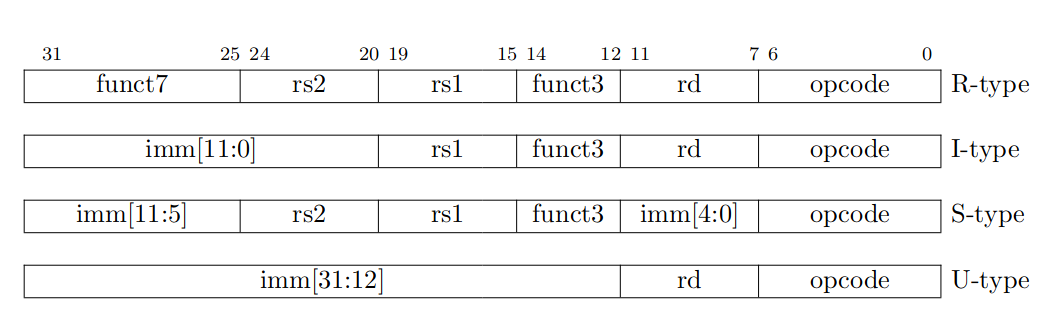
\includegraphics[width=1.0\textwidth]{img/RISCV_4_Commands.png}
    \caption{Основные форматы команд 32-разрядного процессора RISC-V}
    \label{command-01}
\end{figure}
Обозначения на рисунке:
\begin{itemize}
    \item \textbf{opcode} — код операции (6 битов)
    \item \textbf{rs1} --- № регистра-источника (5 битов)
    \item \textbf{rs2} --- № регистра-операнда (5 битов)
    \item \textbf{rd} --- № регистра-приёмника (5 битов)
    \item \textbf{imm[11:0]} --- непосредственный операнд размером в 12 битов (В случае, когда непосредственное значение определяет «приёмник» (смещен адреса для «близкого» перехода или записи результата в память), 12 битов целиком в поле rd не помещаются, и его приходится «распиливать» (инструкция типа S). Непосредственный операнд всегда знаковый, и его знак всегда приходится на 31-й бит)
    \item \textbf{imm[31:12]} --- непосредственный операнд размером в 20 битов. Используется в инструкциях типа U для заполнения старших двадцати битов регистра (в операциях «далёкого» перехода и как дополнительная инструкция при записи в регистр полного 32-разрядного непосредственного операнда)
    \item \textbf{funct} --- поле функции (6 битов), используется для разных инструкций, у которых код операции одинаковый. Например, все арифметические инструкции типа I имеют одинаковый opcode OP-IMM (чему он равен?), а различаются полем funct. По-видимому, для эффективной реализации R-команд в конвейере удобнее не декодировать опкод, а по-быстрому сравнить его с нулём, и получать значения регистров, параллельно декодируя функцию, чтобы потом её применить.
\end{itemize}

\subsubsection{Мнемоника команд}

Изначально мнемонику команд можно рассмотрить в системе помощи RARS (раздел Basic Inctructions), где в алфавитном порядке представлены практически все команды. Однако этот формат не вполне удобен для постепенного изучения. Поэтому можно сослаться на пару таблиц, в которых команды систематизирован, но представлены без описания. Можно предложить совместное использование этой справочной информации по мере необходимости. В принципе в методе по самостоятельной работе данный материал стоит систематизировать и выложить в LMS. Начало положено. Там можно сделать все в соответствии с порядком изучения.
Обе таблицы с кратким представлением набора команд (\verb|RARS_reference_card.pdf| и \verb|riscv-reference-card.pdf|) я положил в каталог \verb|info| на \verb|gitflic|.

\subsubsection{Псевдокоманды}

Рассмотрение мнемоники псевдокоманд в целом можно осуществить по той же схеме, что и изучение команд. Их достаточно обширный список представлен в системе помощи. Однако, в связи с тем, что речь идет о первоначальном знакомстве, вряд ли имеет смысл на этой мнемонике долго останавливаться. Также можно обратиться к отображениям в дополнительной информации. Или к методическим материалам для самостоятельного изучения (надеюсь, что соответствующие материалы и презентации разработаем).

\section{Область кода}

Можно еще раз подчеркнуть адресное пространство, в котором располагается программный код. Также отметить, что при описании на ассемблере соответствующими директивами (\verb|.data| и \verb|.text|) можно чередовать код и данные, а ассемблер разместит их в своих областях.

\subsection{Методы адресации данных, используемые в ассемблере RISC-V}

Пояснить основные методы адресации, которые используются в процессоре на уровне обмена с памятью. Показать необходимость использования адресации в памяти как для обращения к данным и их пересылки, так и для организации управления вычислениями.

\subsubsection{Ветвления и переходы}

Можно рассмотреть базовые инструкции вида <<сравнить и перейти>> \\ (\verb|beq/bne /blt/bge/btlu/bgeu|. Все остальные инструкции вида \verb|b*|, включая безусловный переход \verb|b| --- это псевдоинструкции, потому что получаются простой перестановкой регистров--операндов или подстановкой регистра \verb|zero| в нужное место. Непосредственный 12-битный операнд используется для хранения смещения относительно текущего адреса. Вычислением этого смещения из метки занимается ассемблер, оно бывает положительное (вперёд) и отрицательное (назад, как в примере). 12 битов хватает на то, чтобы сделать переход на 4 килобайта кода (4, а не 2, потому что адрес всегда кратен 2 и самый младший бит просто не хранится).

Пример перехода по постусловию (из материалов Курячего):
\begin{verbatim}
    # Переходы по постусловию
    li      s2 10           # Граница счётчика
    li      s1 1            # Счётчик
    loop:   li      a7 1            # Вывод счётчика
    mv      a0 s1
    ecall
    addi    s1 s1 1         # Увеличение
    blt     s1 s2 loop      # Сравнение счётчика и границы и переход
    li      a7 10           # Останов
    ecall
\end{verbatim}
Можно рассмотреть, что получится после компиляции и выделить непосредственные 12--разрядные операнды

Пример перехода по предусловию с длинным переходом (из материалов Курячего):
\begin{verbatim}
    li      s2 10
    li      s1 1            # Инициализация
    loop:   bge     s1 s2 final     # Проерка условия
    li      a7 1            # Тело
    mv      a0 s1
    ecall                   # Вывод целого
    li      a7 11
    li      a0 10
    ecall                   # Вывод перевода строки
    addi    s1 s1 1         # Изменение
    j       loop            # Дополнительный переход
    final:  li      a7 10
    ecall\end{verbatim}
Безусловный переход может называться b, а может j — это одна и та же псевдоинструкция. Это инструкция <<длинного>> перехода типа J (20 битов, т. е. по мегабайту в обе стороны с учётом ещё одного младшего бита). Есть более подробное описание у Курячего. Но думаю, что сильно на данном этапе заморачиваться не стоит, так как пока программы простые. А в методических указаниях можно более подробно описать. Возможно, что данный пример можно пока тоже не рассматривать...

\subsubsection{Косвенная адресация и массивы}

Как вариант доступа к данным --- записать полный абсолютный адрес в регистр, и воспользоваться инструкцией, которая работает с памятью, находящейся по этому адресу. Пример использования псевдоинструкции \verb|lw метка| (из Курячего):
\begin{verbatim}
    .data
    .word   0x1223344
    var:    .word   0xdeadbeef
    addr:   .word   var
    .text
    lw      t1 var
    lw      t2 addr
    lw      t3 (t2)
    lw      t4 4(t2)
    lw      t5 -4(t2)
\end{verbatim}

Результаты компиляции:
\begin{verbatim}
    Address    Code        Basic                     Source

    0x00400000  0x0fc10317  auipc x6,0x0000fc10   6   lw      t1 var
    0x00400004  0x00432303  lw x6,0x00000004(x6)
    0x00400008  0x0fc10397  auipc x7,0x0000fc10   7   lw      t2 addr
    0x0040000c  0x0003a383  lw x7,0x00000000(x7)
    0x00400010  0x0003ae03  lw x28,0x00000000(x7) 8   lw      t3 (t2)
    0x00400014  0x0043ae83  lw x29,0x00000004(x7) 9   lw      t4 4(t2)
    0x00400018  0xffc3af03  lw x30,0xfffffffc(x7) 10  lw      t5 -4(t2)
\end{verbatim}
\begin{itemize}
    \item Инструкция \verb|auipc| формирует в регистре \verb|t1| (он же \verb|x6|) адрес, по которому лежит интересующее нас значение.
    \item далее \verb|lw| выбирает это значение из памяти, попутно скорректировав его смещением 4, и кладёт в тот же регистр \verb|t1|.
    \item По метке \verb|addr| размещается метак \verb|var|, то есть адрес \verb|0x10010004|.
    \item Он оказывается в регистре \verb|t2| тем же способом, каким \verb|0xdeadbeef| оказалось в \verb|t1|.
    \item После этого с помощью явно указанного смещения в инструкции \verb|lw| получаем в разных регистрах содержимое памяти по адресам \verb|0x10010004|, \verb|0x10010008| и \verb|0x10010000| сооответственно.
\end{itemize}

Косвенная адресация — единственный способ обработки массива. Массив — это адрес в памяти и длина (количество элементов * размер одного элемента). В примере массив слов расписывается последовательными значениями:
\begin{verbatim}
    .data
    array:  .space  64
    arrend:
    .text
    la      t0 array
    la      t1 arrend
    li      t2 1
    loop:   sw      t2 (t0)
    addi    t2 t2 1
    addi    t0 t0 4
    bltu    t0 t1 loop
    li      a7 10           # Останов
    ecall
\end{verbatim}
Пояснить каким образом формируется адрес текущего элемента массива. Также акцентировать внимание, что остановка осуществляет не по числу элементов в массиве (что тоже возможно), а по достижению адреса \verb|arrend|, фиксирующего ячейку после завершения массива.

\subsection{Моделирование на ассемблере различных операторов управления}
Учитывая, что основные элементы и команды управления уже показаны, можно кратко остановиться на примерах имитации базовых операторов управления языков высокого уровня. Думаю, что для понимания достаточно их прогона. Тоже будут в LMS.

\subsubsection{Оператор if}
\begin{verbatim}
    # if (t0 == 0) {
        #     t1 = 1;
        # } else if (t0 < 0) {
        #     t1 = 2;
        # } else if (t0 >= 10) {
        #     t1 = 3;
        # } else {
        #     t1 = 4;
        # }
    main:
    li   a7, 5
    ecall
    mv   t0, a0
    if_0:
    bnez t0, if_less_0
    li   t1, 1
    j    end_if
    if_less_0:
    bgtz t0, if_greater_10
    li   t1, 2
    j    end_if
    if_greater_10:
    li   t3, 10
    ble  t0, t3, else
    li   t1, 3
    j    end_if
    else:
    li   t1, 4
    end_if:
    li   a7, 1
    mv   a0, t1
    ecall
\end{verbatim}

\subsubsection{Оператор while}
\begin{verbatim}
    # while((t0 = read_int()) != 0) {
        #    print_int(t0)
        #    print_char('\n')
        # }
    while:
    li   a7, 5
    ecall
    mv   t0, a0
    beqz a0, end_while
    li   a7, 1
    ecall
    li   a7, 11
    li   a0, '\n'
    ecall
    j    while
    end_while:
\end{verbatim}

\subsubsection{Оператор for}
\begin{verbatim}
    # for (t0 = 0; t0 < t1; ++t0) {
        #     print_int(t0)
        #     print_char('\n')
        # }
    for:
    li   a7, 5
    ecall
    mv   t1, a0
    mv   t0, zero
    next:
    beq  t0, t1, end_for
    mv   a0, t0
    li   a7, 1
    ecall
    li   a7, 11
    li   a0, '\n'
    ecall
    addi t0, t0, 1
    j    next
    end_for:
\end{verbatim}

\section{Имитация в эмуляторе системных вызовов. Аналогии системных вызовов в операционных системах}

Разговор о том, что системные вызовы эмулятора отличаются от системных вызовов ОС идет постоянно, начиная с первого семинара. Поэтому в ходе этого и последующих семинаров дополнительно стоит пояснять только новые вызовы и отсылать к системе помощи эмулятора, в которой хорошо описаны принципы их работы. Поэтому здесь особо акцентироваться не на чем. Только повторять ранее сказанное, избегая при этом занудства...
Может быть не имеет смысла держать этот пункт в теме.

\section{Примеры простых целочисленных алгоритмов}

После рассмотрения команд управления можно рассмотреть пару простых алгоритмов. Ниже представлены в качестве примеров нахождение числа Фибоначчи и вычисление наибольшего общего делителя двух чисел (алгоритм Евклида). В целом заострять внимание на них сильно не стоит в связи с очевидностью решений. Но прогнать их студентам имеет смысл. Возможно, с разными исходным данным, чтобы показать отсутствие обработки некорректных входных данных. Программы также будут находиться в LMS.

\subsection{Вычисление числа Фибоначчи}
\begin{verbatim}
    #
    # Example that calculates the Fibonacci sequence.
    #
    main:
    mv   t0, zero
    li   t1, 1

    li   a7, 5
    ecall
    mv   t3, a0
    fib:
    beqz t3, finish
    add  t2, t1, t0
    mv   t0, t1
    mv   t1, t2
    addi t3, t3, -1
    j    fib
    finish:
    li   a7, 1
    mv   a0, t0
    ecall
\end{verbatim}

\subsection{Алгоритм Евклида}
\begin{verbatim}
    # Calculates the greatest common divisor of
    # two values using the Euclidean algorithm.
    # int gcd(int a, int b) {
        #    while (a != b)
        #        if a > b
        #            a = a - b;
        #        else
        #            b := b - a;
        #    return a;
        # }

    .data
    arg01:  .asciz "Input 1st number: "
    arg02:  .asciz "Input 2nd number: "
    result: .asciz "Result = "
    ln:     .asciz "\n"

    .text
    main:
    la 	a0, arg01   # Подсказка для ввода первого числа
    li 	a7, 4       # Системный вызов №4. Ввод строки в стиле Си
    ecall

    li  a7, 5       # Системный вызов №5. Ввод целого
    ecall
    mv  t1, a0

    la 	a0, arg02   # Подсказка для ввода второго числа
    li 	a7, 4       # Системный вызов №4. Ввод строки в стиле Си
    ecall

    li  a7, 5
    ecall
    mv  t2, a0

    loop:
    beq t1, t2, finish

    slt t0, t1, t2
    bne t0, zero, if_less

    sub t1, t1, t2
    b   loop

    if_less:
    sub t2, t2, t1
    b   loop

    finish:
    la a0, result   # Подсказка для выводимого результата
    li a7, 4        # Системный вызов №4
    ecall

    li  a7, 1 		# Системный вызов №1 — вывести десятичное число
    mv  a0, t1
    ecall

    la 	a0, ln      # Перевод строки
    li  a7, 4       # Системный вызов №4
    ecall

    li      a7 10   # Системный вызов №10 — останов программы
    ecall
\end{verbatim}

\section{Домашнее задание}

\subsection{До 10 баллов}

Разработать на ассемблере RARS программу, осуществляющую целочисленное деление для 32-разрядных целых чисел со знаком, используя операции вычитания, ветвления и циклы. Исходные делимое и делитель вводятся с клавиатуры в десятичной системе счисления. Полученные в результате деления частное и остаток необходимо вывести на консоль эмулятора. Остаток от деления вычисляется по правилам, используемых при выполнения операции вычисления остатка (\verb|%|) в языках программирования \verb|C/C++|. При делении учитывать знаки операндов и результатов, а также возможность ошибок при делении на ноль.

В отчете привести примеры скриншотов консоли, демонстрирующие все возможные комбинации тестового покрытия.

Рекомендации. Предварительно данную программу можно отработать на языках более высокого уровня (рекомендуется использовать C/C++).



% --- Семинар 04. Семинар 04. Подпрограммы. Стек. Кадр стека. Параметры. Локальные переменные ---
\chapter[Целочисленная арифметика. Массивы]{Семинар 04. Целочисленная арифметика. Одномерные и многомерные массивы. Простые алгоритмы}

Целью семинара изучение команд, обеспечивающих обработку целочисленных данных со знаком и без знака, организацию управления в программах, использующих целочисленную арифметику. Распределение памяти под целочисленные одномерные и многомерные массивы, организации доступа к элементам массивов различной размерности.

Проведение семинара предполагается по следующему плану:
\begin{enumerate}
    \item Обзор команд, обеспечивающих поддержку целочисленной арифметики.
    \item Организация в памяти одномерных массивов и методы доступа к этим массивам.
    \item Примеры работы с одномерными массивами.
\end{enumerate}

\section{Сценарий семинара}


\subsection{Обзор команд, обеспечивающих поддержку целочисленной арифметики}

Предлагается кратко охарактеризовать список основных и дополнительных команд процессора, реализующих базовую арифметику и логику для 32-х разрядной архитектуры. В конспекте лекций я их разбил на отдельные небольшие таблицы. Думаю, что после завершения перевода они перенесутся в методу для самостоятельной работы (сами списки взяты из системы помощи RARS).

Но в целом понятно, что на все эти команды разом обращать внимание бесполезно поэтому проще продемонстрировать те схемы, которые в сокращенном виде представляют команды процессора. Одна из них --- это список команд в эмуляторе RARS (рисунок~\ref{ref-rars-commands}). При необходимости их описание можно прочитать в системе помощи эмулятора.

\begin{figure}[htbp]
    \centering
    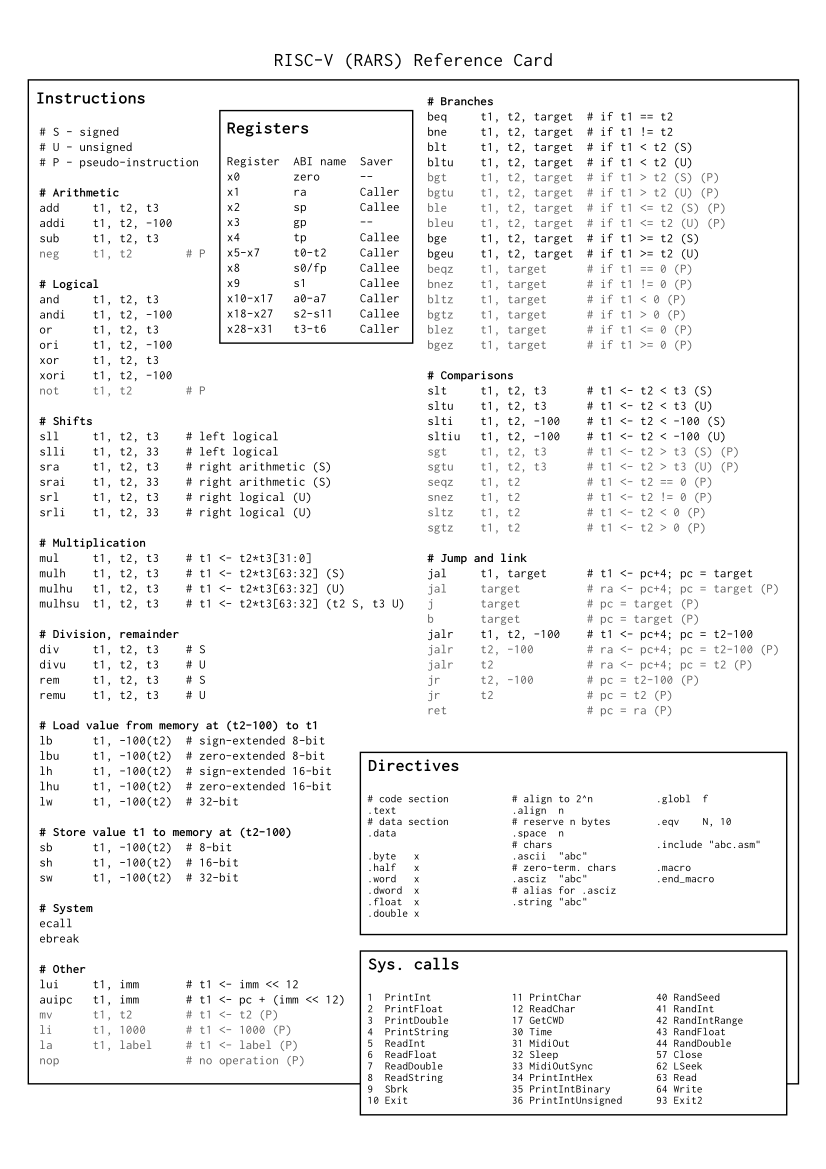
\includegraphics[width=1.0\textwidth]{img/RARS_reference_card.png}
    \caption{Команды 32-разрядного процессора RISC-V, реализованные в эмуляторе RARS}
    \label{ref-rars-commands}
\end{figure}

Другая схема дает более полное описание уже не только RV32I, но и других вариантов. Но там легко выделить изучаемый процессор. И возможно, что она является более наглядной. Занимает, правда две страницы (рисунок~\ref{ref-riscv-commands-01} и рисунок~\ref{ref-riscv-commands-02}). Основное достоинство --- более четко расписаны операнды и приводятся типы форматов команд. Но в целом на больше будет интересовать первый документ.

\begin{figure}[htbp]
    \centering
    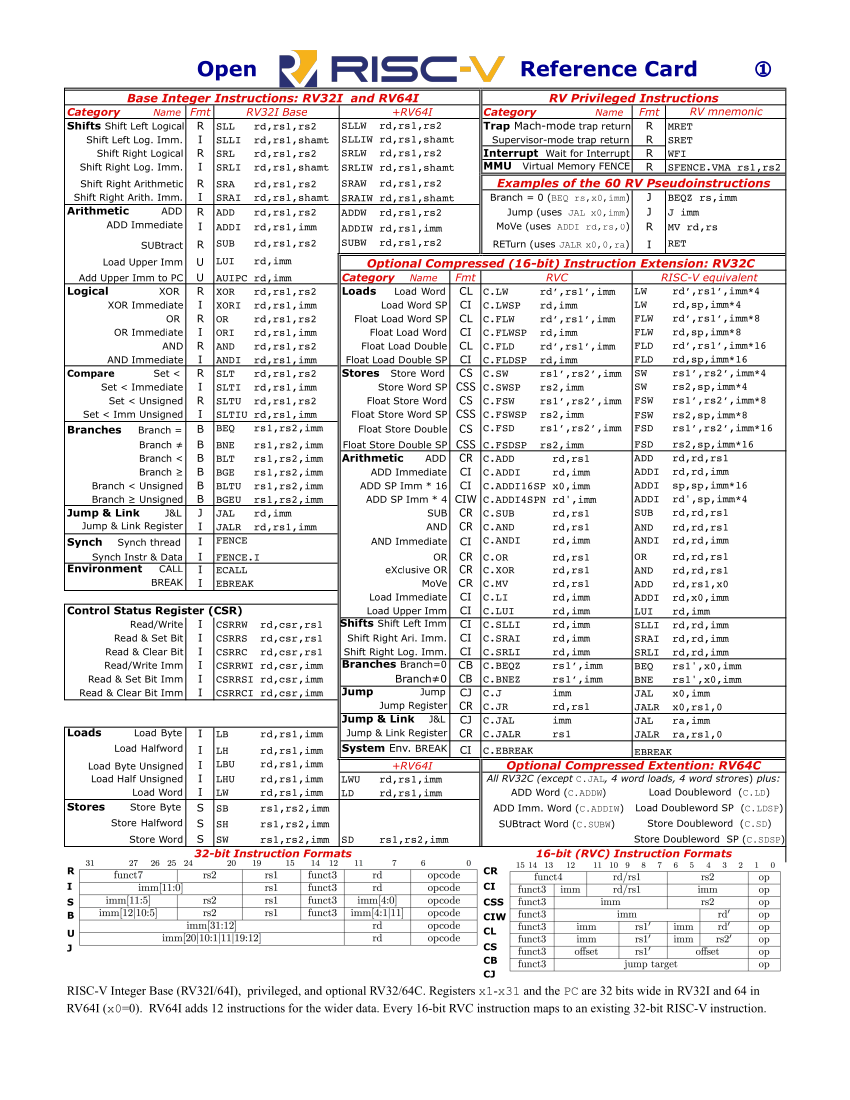
\includegraphics[width=1.0\textwidth]{img/riscv-reference-card-01.png}
    \caption{Команды процессора RISC-V (начало)}
    \label{ref-riscv-commands-01}
\end{figure}

\begin{figure}[htbp]
    \centering
    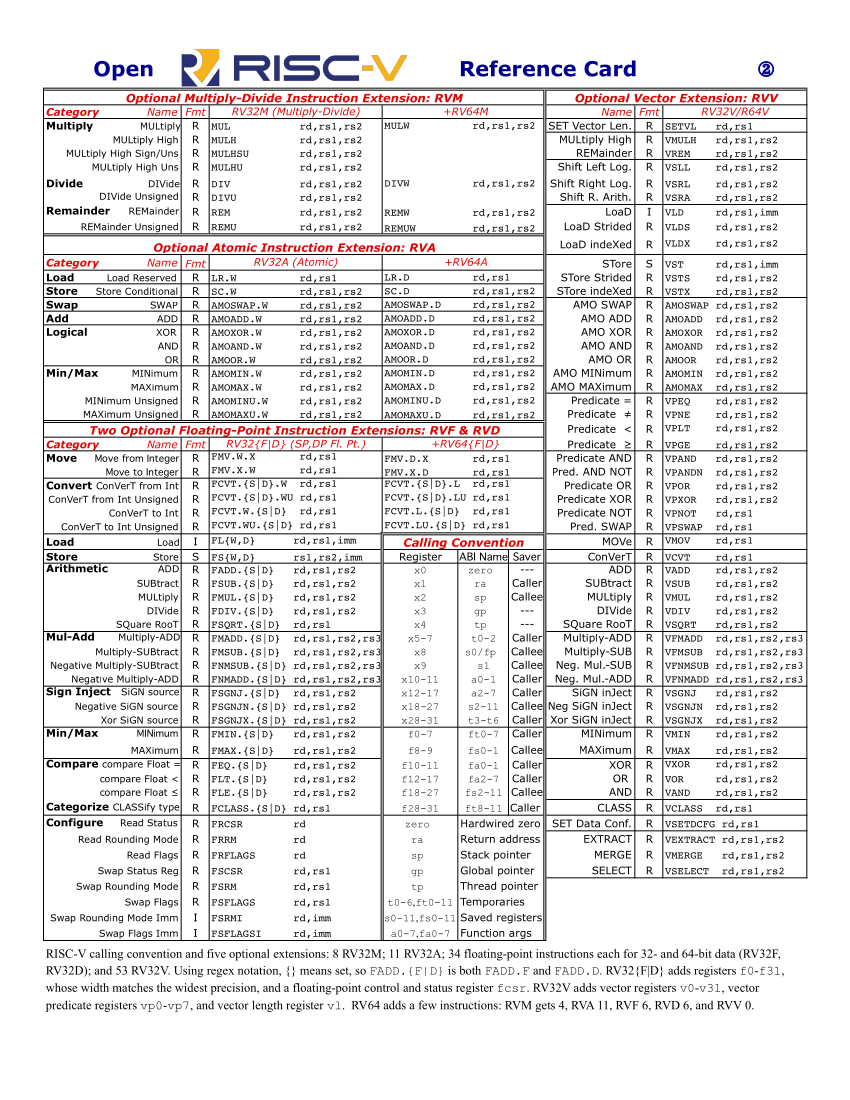
\includegraphics[width=1.0\textwidth]{img/riscv-reference-card-02.png}
    \caption{Команды процессора RISC-V (окончание)}
    \label{ref-riscv-commands-02}
\end{figure}

Обе схемы выложены в LMS. Поэтому при необходимости их можно будет скачать. В принципе на второй схем можно пояснить, что команды целочисленного умножения и деления являются для 32-х разрядной архитектуры опциональными (не знаю, насколько это важно).

Основная идея --- сказать, чтобы не пугались, что их много. Не все будут нужны и не сразу, а постепенно. Главное - ориентироваться в базовом списке в основных группах и при необходимости читать о них в системе помощи.

Лалее по ходу объяснения можно обращаться к различным группам команд, когда потребуются различия в представлении:
\begin{itemize}
    \item знаковых и беззнаковых чисел;
    \item байтов, слов, двойных слов;
    \item и т.д.
\end{itemize}

\section{Организация в памяти одномерных массивов и методы доступа к этим массивам}

Изначально можно представить простую программу на Си, в которой, как и в последующей ассемблерной решается задача формирования и вывода элементов целочисленного массива:

\begin{verbatim}
    #include <stdio.h>

    int array[16];

    int main()
    {
        fill:
        for(int i = 0; i < 16; ++i) {
            array[i] = i+1;
        }
        printf("--------\n");
        out:
        for(int i = 0; i < 16; ++i) {
            printf("%d\n", array[i]);
        }
        return 0;
    }
\end{verbatim}

\subsection{Работа с одномерными массивами}
Можно начать с пояснения того, что формирование индекса элемента массива как отдельно рассматриваемого целого числа, увеличивающегося на 1 в принципе возможно. Однако в ассемблере предпочтительнее манипулировать непосредственно с адресным пространством нужной величины, а не умножать каждый раз на величину слова, так как операция умножения затратна по времени. Она даже не входит в базовый набор. Хотя можно ислпользовать сдвиги вместо умножения. Но все равно это лишние команды (но при желании пусть используют).
Основной режим работы - использование косвенной адресации с индексацией относительно начала массива.

Показать, что для выделения массива достаточно задать память, выделяемую под него различными способами:
\begin{itemize}
    \item можно выделить пространство требуемого размера;
    \item при наличии заранее предопределенных значений элементов можно их перечислить;
    \item при неизвестном числе элементов можно зарезервировать некоторый большой кусок памяти, а количество элементов задавать числом, меньшим выделенного размера, которое (как и впрограмме на Си) может служить окраничителем цикла при формировании массива;
    \item можно выделить память под массив на куче после получения числа элементов в массиве.
\end{itemize}
В качестве стартового примера можно опять обратиться к лекциям Г. Курячего:
\begin{verbatim}
.data
sep:    .asciz  "--------\n"    # Строка-разделитель (с \n и нулём в конце)
.align  2                       # Выравнивание на границу слова
array:  .space  64              # 64 байта
arrend:                         # Граница массива
.text
la      t0 array                # Счётчик
la      s1 arrend
li      t2 1            # Число, которое мы будем записывать в массив
fill:   sw      t2 (t0)         # Запись числа по адресу в t0
addi    t2 t2 1         # Изменим число
addi    t0 t0 4         # Увеличим адрес на размер слова в байтах
bltu    t0 s1 fill      # Если не вышли за границу массива
la      a0 sep          # Выведем строку-разделитель
li      a7 4
ecall
la      t0 array
out:    li      a7 1
lw      a0 (t0)         # Выведем очередной элемент массива
ecall
li      a7 11           # Выведем перевод строки
li      a0 10
ecall
addi    t0 t0 4
blt     t0 s1 out
li      a7 10           # Останов
ecall
\end{verbatim}
На основе этого примера можно пояснить, что при выделении под массив, который заполняется полностью, можно не использовать его размерность, а указывать метку, задающую ограничительный адрес.

На примере этой программы можно предложить модификации на занятиях, в которых заполнение осуществляется побайтно и по 16 разрядным словам (эти примеры лежать не будут, студенты должны сделать самостоятельно). При этом следует откорректировать не только команду загрузки в память, но и чтения из нее (при выводе).

Пример для генерации байтового массива:
\begin{verbatim}
    .data
    sep:    .asciz  "--------\n"    # Строка-разделитель (с \n и нулём в конце)
    .align  2                       # Выравнивание на границу слова
    array:  .space  64              # 64 байта
    arrend:                         # Граница массива
    .text
    la      t0 array                # Счётчик
    la      s1 arrend
    li      t2 1            # Число, которое мы будем записывать в массив
    fill:   sb      t2 (t0)         # Запись числа по адресу в t0
    addi    t2 t2 1         # Изменим число
    addi    t0 t0 1         # Увеличим адрес на размер слова в байтах
    bltu    t0 s1 fill      # Если не вышли за границу массива
    la      a0 sep          # Выведем строку-разделитель
    li      a7 4
    ecall
    la      t0 array
    out:    li      a7 1
    lb      a0 (t0)         # Выведем очередной элемент массива
    ecall
    li      a7 11           # Выведем перевод строки
    li      a0 10
    ecall
    addi    t0 t0 1
    blt     t0 s1 out
    li      a7 10           # Останов
    ecall
\end{verbatim}
Аналогично можно быстро сделать модификацию и для 16-разрядных слов, изменяя только команды чтения и записи в память.

Помимо этого можно предложиеть модифицировать первую программу так, чтобы вводить в память ограниченное число элементов, заданных максимально допустимым числом. По примеру следующей программы на Си:
\begin{verbatim}
#include <stdio.h>

int array[16];
int n;

int main()
{
    in:
    printf("n = ? ");
    scanf("%d", &n);
    if(n > 16 || n < 1) {
        printf("n = %d is incorrect!\n", n);
        return 1;
    }
    fill:
    for(int i = 0; i < n; ++i) {
        array[i] = i;
    }
    printf("--------\n");
    out:
    for(int i = 0; i < n; ++i) {
        printf("%d\n", array[i]);
    }
    return 0;
}
\end{verbatim}
В этом случае может получиться примерно такое (но необязательно одинаково, так как возможны варианты):

\begin{verbatim}
    .data
    sep:    .asciz  "--------\n"    # Строка-разделитель (с \n и нулём в конце)
    prompt: .asciz  "n = ? "         # Подсказка для ввода числа
    error:  .asciz  "incorrect n!\n"  # Сообщение о некорректном вводе
    .align  2                       # Выравнивание на границу слова
    n:	.word	0		# Число введенных элементов массива
    array:  .space  64              # 64 байта
    .text
    in:
    la 	a0, prompt      # Подсказка для ввода числа элементов массива
    li 	a7, 4           # Системный вызов №4
    ecall
    li      a7 5            # Системный вызов №5 — ввести десятичное число
    ecall
    mv      t3 a0           # Сохраняем результат в t3 (это n)
    ble     t3 zero fail    # На ошибку, если меньше 0
    li      t4 16           # Размер массива
    bgt     t3 t4 fail      # На ошибку, если больше 16
    la	t4 n		# Адрес n в t4
    sw	t3 (t4)		# Загрузка n в память на хранение

    la      t0 array        # Указатель элемента массива
    li      t2 1            # Число, которое мы будем записывать в массив
    fill:   sw      t2 (t0)         # Запись числа по адресу в t0
    addi    t2 t2 1         # Изменим число
    addi    t0 t0 4         # Увеличим адрес на размер слова в байтах
    addi    t3 t3 -1        # Уменьшим количество оставшихся элементов на 1
    bnez    t3 fill         # Если осталось больш 0
    # bltu    t0 s1 fill      # Если не вышли за границу массива
    la      a0 sep          # Выведем строку-разделитель
    li      a7 4
    ecall

    lw	t3 n		# Число элементов массива
    la      t0 array
    out:    li      a7 1
    lw      a0 (t0)         # Выведем очередной элемент массива
    ecall
    li      a0 '\n'         # Выведем перевод строки
    li      a7 11
    ecall
    addi    t0 t0 4
    addi    t3 t3 -1        # Уменьшим количество оставшихся элементов на 1
    bnez    t3 out          # Если осталось больше 0
    # blt     t0 s1 out
    li      a7 10           # Останов
    ecall
    fail:
    la 	a0, error       # Сообщение об ошибке ввода числа элементов массива
    li 	a7, 4           # Системный вызов №4
    ecall
    li      a7 10           # Останов
    ecall
\end{verbatim}

\debate[Примечание.]{На самом деле у меня на отработку этой простой программы ушло немало времени, включая отладку. Возможно стоит, после небольшой паузы, просто продемонстрировать ее решение. Нужно прикинуть хронометраж. Также решил убрать работу с многомерными массивами. Их не будет в задании. Вряд ли на стоит заострять внимание.}

\section{Домашнее задание}

\subsection{До 8 баллов}

Написать программу, осуществляющую суммирование целочисленных элементов одномерного массива. Количество элементов в массиве может варьироваться от 1 до 10. Сами элементы вводятся с клавиатуры. Значение суммы также выводится в консоль эмулятора RARS. Необходимо контролировать, чтобы число вводимых элементов не превышало максимально допустимое. В случае, когда возникает переполнение, необходимо вывести последнее корректное значение суммы и число просуммированных при этом элементов. Суммирование осуществлять после размещения массива в памяти.

\subsection{Опционально до +2 баллов}

Подсчитать количество четных и нечетных элементов в обрабатываемом массиве. Подсчет осуществлять в массиве, который уже расположен в памяти.
% --- Семинар 05. Немного об ассемблере. Многофайловые программы. Директивы. Макросы ---
\chapter[Подпрограммы. Начало]{Семинар 05. Подпрограммы. Передача параметров}

Целью семинара является изучение использования подпрограмм на уровне систмы команд.
На занятии предполагается рассмотреть следующие темы:
\begin{enumerate}
    \item Особенности вызова подпрограмм в системе команд RISC-V и возврата из подпрограмм.
    \item Использование подпрограмм без параметров и с параметрами. Достоинства и недостатки. Примеры.
    \item Соглашения о передаче фактических параметров и возврате результатов в архитектуре RISC-V.
\end{enumerate}

\section{Особенности вызова подпрограмм и возврата из подпрограмм}
\debate[Примечание]{Данную тему в первой итерации предлагается заимствовать из Г.~Курячего, что в общем-то уже и сделано. В дальнейшем, думаю, стоит уточнить примеры. Помимо этого вставить дополнительные более сложные примеры, раскрывающие особенности различных моментов использования подпрограмм. Все необходимые материалы уже сгруппированы в соответствующей презентации.}

В целом изложение выглядит следующим образом:
\begin{itemize}
    \item определение подпрограммы;
    \item отличие ассемблерных подпрограммы от подпрограмм, процедур, функций языков высокого уровня;
    \item описание подпрограмм в ассемблере процессора RISC-V (эмулятора RARS);
    \item команды и псевдокоманды вызова подпрограмм;
    \item команды и псевдокоманды возврата из подпрограмм
\end{itemize}

\section{Использование подпрограмм и без параметров. Достоинства и недостатки. Примеры}

Основной акцент сделать на примерах (изложены в презентациях). Показать на эмуляторе в пошаговом режиме, что происходит:
\begin{itemize}
    \item пример использования вызовов \verb|jal|  и \verb|jalr|;
    \item пример с отрезками, составляющими стороны треугольника (на нем можно показать изощренность возврата, что не всегда удобно в практическом решении из-за появления избыточных зависимостей);
\end{itemize}

\section{Соглашения о передаче фактических параметров и возврате результатов}

Рассказать об основных соглашениях, моделирующих передачу параметров внутрь подпрограмм, аналогичную использованию параметров в процедурах и функциях. Рассказать о соглашении использования регистров \verb|a*| как для передачи параметров, так и возврата результатов (\verb|a0|, \verb|a1|). Лишний раз напомнить, для чего используются соглашения.

\section{Выдача задания №~1}

Судя по дыре в расписании учебных занятий, минисессия будет проходить с 30 октября. Думаю, что на выполнение первого задания можно выделить 3 полных недели, поставив дедлайн 15 октября 23:59. График заданий сформирован и выложен в ЛМС. Также уже выложены варианты и требования к выполнению заданий. Все это ляжет и в репозиторий. Генератор вариантов тоже лежит. В принципе всю информацию по вариантам можно выложить в чаты и зафиксировать в текущих ведомостях. Основное --- объявить дефакто, что задание роздано. Я об этом также объявлю на лекции.

Для групп, которые в пятницу, распределить задания можно раньше. Хоть в понедельник, разослав им список номеров по группам. По почте каждой группе отдельно предпочтительнее. Я наверное тоже своей группе дополнительно вышлю, так как тогда будет документ, против которого возразить будет сложно.

\section{Домашнее задание}

Домашнее задание завязано на второй семинар по данной теме, который по сути является продолжением. Тема разбита и немного увеличена по содержанию из-за добавления семинарских занятий в этом году.

% --- Семинар 06. Математический сопроцессор. Арифметика с плавающей точкой ---
\chapter[Подпрограммы. Окончание]{Семинар 06. Подпрограммы. Стек. Кадр стека. Параметры. Локальные переменные}

Целью семинара является продолжение изучения подпрограмм на уровне систмы команд. Основной упор при этом делается на роль стека в современном программировании не только на ассемблере, но и в языках высокого уровня.

На занятии предполагается рассмотреть следующие темы:
\begin{enumerate}
    \item Пояснение специфики использования стека и его организации в целом. Привязаки стека к памяти.
    \item Особенности работы со стеком в RISC-V. Основные команды. Стек как хранилище, альтернативное общей памяти.
    \item Использование стека для дополнительных фактических параметров.
    \item Использование стека для локальных переменных подпрограммы и дополнительных фактических параметров.
    \item Разработка рекурсивных подпрограмм.
    \item Соглашения о вызовах подпрограмм, использовании регистров. Кадр стека.
    \item Выдача индивидуального задания №~1. Установка сроков и регламента сдачи индивидуальных заданий.
\end{enumerate}

\section{Общая специфика использования стека}
В принципе уже прописано в презентации. Скорее всего он также изучен в дисциплине "Алгоритмы и структуры данных". Поэтому сильно акцентироваться не стоит. Достаточно дать основные определения. Можно подчеркнуть, что стек на уровне архитектур ВС обычно представляет собой линейное пространство памяти. Оно может быть выделено в любом месте. Но чаще всего в верхних адресах. Стек может расти с нижних адресов вверх, хотя чаще реализуется таким образом, что с верхних адресов растет вниз навстречу куче.

Остановиться на специфике размещения стека в памяти эмулятора RARS.

\section{Особенности работы со стеком в RISC-V}
Пояснить, что в принципе для работы со стеком нет специальных команд и любой регистр может являться указателем на вершину стека. Вместе с тем, под указатель стека соглашением выделен регистр \verb|x2|, который имеет псевдоним \verb|sp|.

Далее на примере (уже есть в презентации) рассмотреть использования стека в пошаговом режиме. Посмотреть в эмуляторе, как изменяются регистры процессора и память, отведенная под стек.

Здесь же можно отметить, что на стеке обычно сохраняется и адрес возврата из подпрограммы, что позволяет организовать иерархические вложенные вызовы подпрограмм, а также обеспечить выполнение рекурсивных подпрограмм.

\section{Использование стека для дополнительных фактических параметров}

Рассказать, что если передаваемых в подпрограмму параметров много, и они не размещаются в регистрах, то обычно используется стек, в который эти параметры и ложатся.


\section{Использование стека для локальных переменных подпрограммы}

Аналогичным образом пояснить использовани и хранение на стеке локальных переменных. Можно также сказать (возможно еще раз), что это сохранение бывает более эффективным, чем в глобальной памяти за счет того, что поддерживает одной командой загрузки в стек или чтения из него по сравнению с обращением по абсолютному адресу.

\section{Разработка рекурсивных подпрограмм}

Показато на примерах работу с рекурсивными подпрограммами.

\section{Соглашения о вызовах подпрограмм, использовании регистров. Кадр стека}

Суммировать материал об основных соглашениях, связанных с организацией подпрограмм, ролевым распределением регистров, выделением регистров \verb|s*| в качеств сохраняемых на стеке и т.д.

\section{Домашнее задание}

\subsection{До 8 баллов}
Разработать программу, определяющую максимальное значение аргумента, при котором результат вычисления факториала размещается в 32-х разрядном машинном слове. Вычисление факториала организовать как подпрограмму с циклом, которая возвращает найденный аргумент в регистре a0. Вывод результатов должна осуществлять главная функция.

\subsection{Опционально до +2 баллов}
Дополнительно реализовать решение предыдущей задачи с использованием рекурсивной подпрограммы вычисления максимального значения аргумента, при котором результат вычисления факториала размещается в 32-х разрядном машинном слове.



% --- Семинар 07. Строки символов. Обработка символьных данных. Файлы ---
\chapter[Дополнительная информация об ассемблере RARS]{Семинар 07. Немного об ассемблере. Директивы. Макросы. Многофайловые программы}

Целью семинара является более глубое погружение в разработку программа на ассемблере RARS для повышения эффективности выполнения последующих домашних и индивидуальных заданий.

\debate[AL]{Принцип тот же самый: не успеем рассмотреть все - переносим на следующий семинар. На самом деле погружение не такое уж глубокое, так как реальные ассемблеры позволяют больше и имеют более развитые средства отладки. Но в курсе по архитектурам ВС это не столь важно. Тем более, что имеющиеся дополнительные средства вполне очевидны и реально позволяют повысить эффективность программирования без изучения каких-либо новых инструментов. Что приходится делать в реальны условиях.}

На занятии предполагается рассмотреть следующие темы:
\begin{enumerate}
    \item Дополнительные директивы, повышающие эффективность написания кода.
    \item Использование макросов.
    \item Создание макробиблиотек.
    \item Сочетание макросов и подпрограмм.
    \item Создание многомодульных программ.
\end{enumerate}

\section{Дополнительные директивы, повышающие эффективность написания кода}

К дополнительным директивам, облегчающим написание кода относятся директивы управления, псевдонимы (алиасы), директивы работы с макроопределениями.

\subsection{Директивы управления}

Директивы управления в основном предназначены для более эффективного управления памятью при написании программ. В большей степени они уже рассматривались. Ниже приведен их список с краткими пояснениями.

Таблица~\ref{table-control-direct} описывает особенности распределения и использования регистров.

\begin{table}[h]
    \caption{Директивы для управления памятью}
    \centering
    \begin{tabularx}{\textwidth}{|c|X|}
        %\rowcolor{lightgray}
        \hline
        \textbf{Обозначение} & \textbf{Соглашения по использованию} \\
        \hline %\hline
        \verb|.align| & Align next data item on specified byte boundary (0=byte, 1=half, 2=word, 3=double) \\
        \hline
        \verb|.ascii| & Store the string in the Data segment but do not add null terminator \\
        \hline
        \verb|.asciz| & Store the string in the Data segment and add null terminator \\
        \hline
        \verb|.byte| & Store the listed value(s) as 8 bit bytes \\
        \hline
        \verb|.data| & Subsequent items stored in Data segment at next available address \\
        \hline
        \verb|.double| & Store the listed value(s) as double precision floating point \\
        \hline
        \verb|.dword| & Store the listed value(s) as 64 bit double-word on word boundary \\
        \hline
        s1 & Сохраняемый регистр 1 (saved register 1) \\
        \hline
        \verb|.eqv| & Substitute second operand for first. First operand is symbol, second operand is expression (like \#define) \\
        \hline
        \verb|.float| & Store the listed value(s) as single precision floating point \\
        \hline
        \verb|.half| & Store the listed value(s) as 16 bit halfwords on halfword boundary \\
        \hline
        \verb|.section| & Allows specifying sections without .text or .data directives. Included for gcc comparability \\
        \hline
        \verb|.space| & Reserve the next specified number of bytes in Data segment \\
        \hline
        \verb|.string| & Alias for .asciz \\
        \hline
        \verb|.text| & Subsequent items (instructions) stored in Text segment at next available address \\
        \verb|.word| & Store the listed value(s) as 32 bit words on word boundary \\
        \hline
    \end{tabularx}
    \label{table-control-direct}
\end{table}

\debate[Примечание.]{Пока комментарии не переведены...}

\subsection{Псевдонимы (алиасы)}

Псевдонимы обычно предназначены для подмены одного текста другим. Чаще всего заменяются константы на идентификаторы этих констант. В RARS для этого используется примитивный макрос, являющийся директивой \verb|.eqv|. Она имеет следующий формат:

\begin{center}
\verb|.eqv имя_псевдонима строка_заменяющая имя|
\end{center}
В результате препроцессорной обработки (обработки текста перед трансляцией) происходит замена этого имени на строку:

\subsection{Директивы для работы с макроопределениями}

\textbf{\textit{Макроподстановка}} — механизм поиска шаблона в тексте и замены его другим текстом. Полученный текст также может содержать шаблоны, так что процесс макроподстановки обычно рекурсивен.

Таблица~\ref{table-macro-direct} описывает директивы, используемые при создании макроопределений.

\begin{table}[h]
    \caption{Директивы для создания макроопределений}
    \centering
    \begin{tabularx}{\textwidth}{|c|X|}
        %\rowcolor{lightgray}
        \hline
        \textbf{Обозначение} & \textbf{Соглашения по использованию} \\
        \hline %\hline
        \verb|.end_macro| & End macro definition.  See \verb|.macro| \\
        \hline
        \verb|.macro| & Begin macro definition.  See \verb|.end_macro| \\
        \hline
    \end{tabularx}
    \label{table-macro-direct}
\end{table}

\subsection{Директивы для работы с многофайловыми программами}

В реальных системах программирования программы собираются из множества модулей, которые хранятся в отдельных файлах, образуя проект. В целом это довольно сложные инструменты. В RARS создание многофайловых проектов решается намного проще.

Таблица~\ref{table-global-direct} описывает директивы, используемые при создании многофайловых проектов.

\begin{table}[h]
    \caption{Директивы для создания многофайловых проектов}
    \centering
    \begin{tabularx}{\textwidth}{|c|X|}
        %\rowcolor{lightgray}
        \hline
        \textbf{Обозначение} & \textbf{Соглашения по использованию} \\
        \hline %\hline
        \verb|.extern| & Declare the listed label and byte length to be a global data field \\
        \hline
        \verb|.global| & Declare the listed label(s) as globl to enable referencing from other files \\
        \hline
        \verb|.globl| & Declare the listed label(s) as global to enable referencing from other files| \\
        \hline
        \verb|.include| & Insert the contents of the specified file.  Put filename in quotes. \\
        \hline
    \end{tabularx}
    \label{table-global-direct}
\end{table}

\section{Использование макросов}

Для демонстрации использования макросов я реализовал сквозной пример на основе алгоритма Евклида. В обычном текстовом представлении он рассматривался и раньше. Его первая версия демонстрирует непосредственно добавление макросов ввода и вывода целых чисел, обертывающих системные вызовы, в файл с кодом основной программы. Пример показывает, как можно просто вставить изначально макросы в программу и как в ней задаются описания параметров и осуществляется вызов макроса.

\textbf{Текст программы находится в каталоге} \verb|euclid/euclid|.

\section{Создание макробиблиотек}

Следующий пример с той же самой программой, но макросы собраны в виде некоторой библиотеки. Библиотека на данном этапе заимствована у Г.\,Курячего. Помимо ввода данных добавлено использование макросов для вспомогательных сообщений. Соответствующее макроопределение демонстрирует локальное использование данных.

\textbf{Текст программы находится в каталоге} \verb|euclid/euclid1|.

\subsection{Макросы с локальными метками}

Многократный вызов макросов требует разрешения конфликтов имен, которые могут повторяться при повторном к ним обращении. Это и метки внутри кода и метки внутри данных. В различны ассемблерах существуют различные подходы решению проблемы дублирования имен. В RARS сделано все просто. Уникальность имен обеспечивается добавлением суффикса \verb|_Mi|. Не всегда это ведет к однозначности. Но в целом для нас достаточно. Другой вариант: можно имя метки задавать через параметр. Тоже не радикальное решение проблемы. Но кратко обсудить можно, используя примеры Курячего, если недостаточно примера с вычислением НОД.

\section{Сочетание макросов и подпрограмм}

Следующий пример демонстрирует использование макросов совместно с подпрограммами. Вычисление НОД выделяется в подпрограмму. В данном примере результат становится ошибочным, так как макросы используют те же регистры, что и подпрограмма.

\textbf{Текст программы находится в каталоге} \verb|euclid/euclid2x|.

Предотвратить подобные конфликты в общем случае сложно, так как часто библиотеки макроопределений пишутся независимо от конкретных программ и, как в нашем случае, могут повторно использоваться. Следовательно их нужно изучать для организации правильного использования. Подобное изучение позволяет предотвратить конфликты по общим ресурсам (регистрам).

Если же регистры, занимаемые макросами, должны использоваться, то можно поступать как и с подпрограммами: сохранять их на стеке. В следующем примере как раз и вводится подобный прием. Перед вызовом конфликтующих макросов осуществляется сохранение в стеке. Для удобства дополнительно разработаны два макроса \verb|push| и \verb|pop|.

\textbf{Текст программы находится в каталоге} \verb|euclid/euclid3|.

Однако не всегда известно, какие макросы и какие регистры используют. Поэтому целесообразно уже при их разработке предусмотреть (как и для подпрограмм) сохранение используемых регистров. В следующем примере сохранение на стеке в ряде макросов, используемых при вычислении НОД, непосредственно используется сохранение. Здесь тоже возможны ситуации, когда это ведет к кофликтам. Например при использовании регистра \verb|a0| Старое значение из стека затирает введенное значение.

\textbf{Текст программы находится в каталоге} \verb|euclid/euclid3|.

Поэтому в примере для работы с этим регистром в следующем примере выделен отдельный макрос. а ввод в любой другой регистр осуществляется с сохранением на стеке значения \verb|a0|, которое может быть в дальнейшем полезно (как в данном примере).

\textbf{Текст программы находится в каталоге} \verb|euclid/euclid4|.

И эта программа работает уже правильно

\subsection{Проблемы макровзрыва и обертывание подпрограмм}

Здесь, думаю, можно сослаться на Курячего, сказав о том, что макроподстановки вместо вызовов процедур удлиняют текст программы. Скорее всего здесь нужно использовать более наглядный пример взрыва, чем НОД, так как в этом примере в основном идет обертки над системными вызовами. Можно подсмотреть у Курячего.

Ну и философски оформить мысль о том, что часто макросами целесообразно обертывать вызовы подпрограмм для сокращения общего размера программы. Несмотря на их удобства. На практике обычно нужно искать баланс, аналогично использованию обычных и \verb|inline| функций в C++.

\section{Создание многомодульных программ}

Многомодульные программы состоят из нескольких единиц компиляции, в каждой из которых сформирован некоторый код реализующий часть решаемой задачи. Для уже существующей программы, вычисляющий наибольший общий делитель, выделим в отдельные файлы подпрограмму нахождения НОД (файл euclid.s) и главную программу, осуществляющую ввод данных, вызов подпрограммы и вывод результата. Для того, чтобы подпрограммы могли быть видны из вне, необходимы их имена отметить директивой \verb|.global| (или с использованием \verb|.globl|, что является дубликатом предыдущей директивы).

\textbf{Текст программы находится в каталоге} \verb|euclid/euclid05mod|.

Для компиляции и выполнения многомодульных программ необходимо в меню эмулятора выставить соответствующие опции (рисунок~\ref{mod-params})
\begin{figure}[htbp]
    \centering
    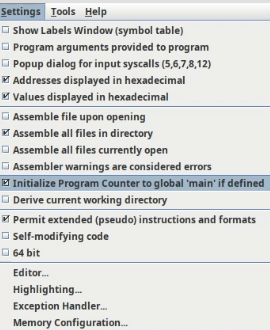
\includegraphics[width=0.4\textwidth]{img/mod-params.png}
    \caption{Установка опций <<Assemble all files in directory>> и <<Initialize Program Counter to global 'main' if defined>> для компиляции и выполнения многофайловых программ}
    \label{mod-params}
\end{figure}

%Settings -> Assemble all files in directory
%Settings -> Initialize Program Counter to global 'main' if defined

\debate[Примечание.]{Кстати, можно многофайловый проект ассемблировать и запустить, используя опции командной строки \texttt{<<p sm>>}. Они являются аналогами опций, устанавливаемых через меню.}

\section{Домашнее задание}

До 8 баллов

Написать программу, осуществляющую суммирование целочисленных элементов одномерного массива. Количество элементов в массиве может варьироваться от 1 до 10. Сами элементы вводятся с клавиатуры. Значение суммы также выводится в консоль эмулятора RARS. Необходимо контролировать, чтобы число вводимых элементов не превышало максимально допустимое. В случае, когда возникает переполнение, необходимо вывести последнее корректное значение суммы и число просуммированных при этом элементов. Суммирование осуществлять после размещения массива в памяти.

При выполнении задания для ввода и вывода массивов, вычисления суммы использовать подпрограммы, размещенные в отдельных файлах общего каталога. Для ввода и вывода отдельных элементов массива использовать макроопределения из библиотеки, рассмотренной на семинарах.

Опционально до +2 баллов

Обернуть подпрограммы ввода массива, вычисления суммы, вывода массива соответствующими макросами, используя эти макросы в основной программе вместо вызова подпрограмм. Эти макросы оформить в отдельном файле, подключаемом к основной программе вместо описания в ней глобальных точек. Подпрограммы должны также оставаться в отдельных файлах.

\textbf{\textit{Срок сдачи задания: до начала восьмого семинарского занятия в каждой из групп.}}



% --- Семинар 08. Обработка исключений ---
\chapter[Арифметика с плавающей точкой. Начало]{Семинар 08. Математический сопроцессор. Арифметика с плавающей точкой}

Целью семинара является изучение подходов к реализации арифметики с плаваюющей точкой за счет применения математического сопроцессора.


На занятии предполагается рассмотреть следующие темы:
\begin{enumerate}
    \item Представление чисел с плавающей точкой.
    \item Организация математического сопроцессора в архитектуре RISC-V.
    \item Псевдоинструкции.
    \item Управление вычислениями в арифметическом сопроцессоре.
    \item Примеры вычислений с плавающей точкой.
\end{enumerate}

\section{Представление чисел с плавающей точкой}

\debate[Примечание]{Следует отметить, что формат чисел с плавающей точкой уже был рассказан на лекции. Поэтому данный материал можно было бы вообще не упоминать. Поэтому я его как бы и не упоминаю. Но можно задать вопрос о том помнят ли студенты, как представляются числа с плавающей точкой в стандарте IEEE-754.Естественно, что больше половины ничего не знают, так как игнорируют лекции. В этой ситуации я планирую просто открыть лекцию и быстро пройтись по ее содержанию одновременно с демонстрацией различных вариантов чисел (включая и крайние) на эмуляторе.}

То есть, как и Г. Курячий, обратиться к RARS и открыть окно эмулятора сопроцессора с плавающей точкой через меню (Tools->Floating Point Representaion). И в этом диалоговом окне имеется визуализация числа с плавающей точной. Можно рассмотреть, что из себя различные значения числа с плавающей точкой представляют. И как они отражаются на двоичное представление. Следует при этом учесть, что это диалоговое окно используется для отображение 32-х разрядных чисел с плавающей точкой. Поэтому, в соответствии с размерностью, ненормализованное представление начинается где-то после $10^{-38}$.

Следует подчеркнуть, что манипулировать можно не только десятичным числом, но и двоичным, выставляя знак, мантиссу и порядок. Таким образом можно показать все варианты (они отображаются в десятичном окне), включая прямое задание ненормализованных чисел, неопределенные значения, плюс/минус бесконечность.

Помимо этого во время выполнения программы данный девайс можно связать с программой и в отладочном режиме просматривать содержимое регистров с плавающей точкой (32-х разрядных значений) в десятичной системе счисления~(рисунок~\ref{fp-representation}).

\begin{figure}[htbp]
    \centering
    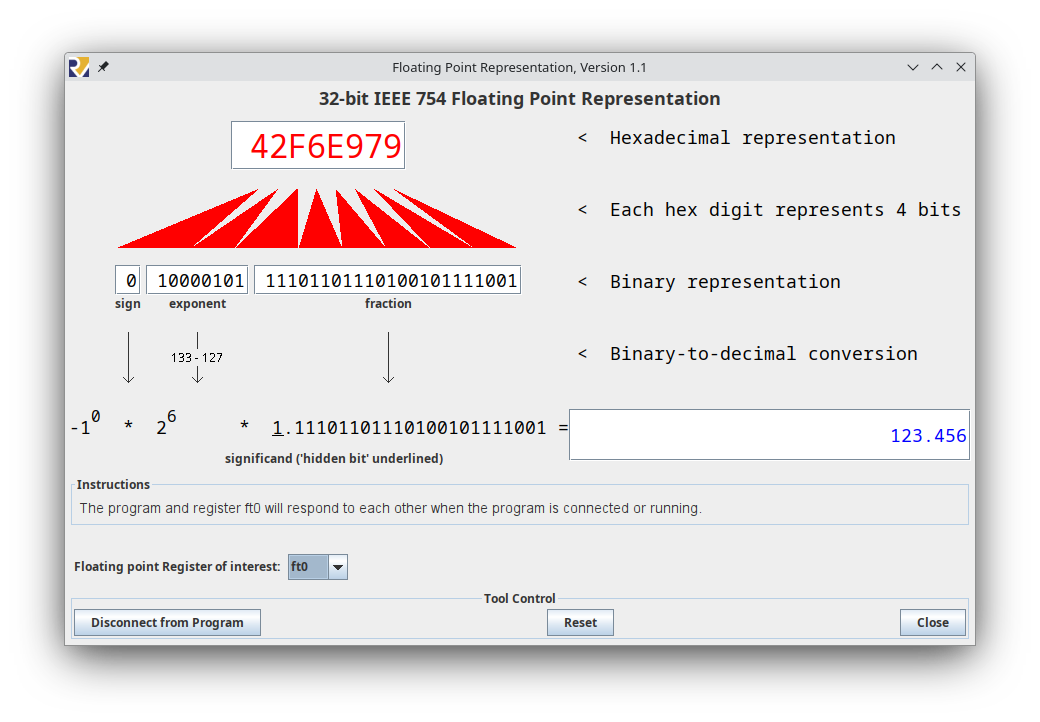
\includegraphics[width=1.0\textwidth]{img/fp-representation.png}
    \caption{Диалоговое окно для просмотра 32-х разрядных чисел с плавающей точкой}
    \label{fp-representation}
\end{figure}

\debate[Примечание]{Курячий показал только манипуляции в десятичном окне. У нас есть время показать больше. Помимо этого можно даже провести небольшое тестирование по этому поводу. Например, дать задание показать, каким образом в двоичном виде будут представлены Пи, Е, и другие числа. Включая не входящие в диапазон 32-х разрядного числа. Можно также поступить наоборот (из двоичной в десятичную), но не знаю, зачем это нужно. Хотя, я им рассказывал, что в LUA использовались ненормализованные числа для представления целочисленной арифметики (52 разряда мантиссы и знак 64-разрядного числа). Можно задать вопрос: какой диапазон целочисленной арифметики может быть представлен в 32-х разрядном числе с плавающей точкой за счет мантиссы и знака.}

\section{Организация математического сопроцессора в архитектуре RISC-V}

Можно остановится на определении сопроцессора (как и у Курячего) как дополнительного устройства, предназначенного для реализации дополнительной функциональности. Сказать, что оно может быть реализовано для различных целей и быть выполнено как на том же кристалле, что и универсальный процессор, или разработано в виде отдельного кристалла (я рассказывал об отдельном Intel 8087), или же быть отдельным устройством (например, видеокарта).

\debate[Можно немного поговорить]{Возможный вопрос: почему не использовать программное решение для арифметики с плавающей точкой на основе целочисленных регистров и моделирования на них любых форматов? Ответ: слишком медленно, а стандартные форматы с плавающей точкой обеспечивают переносимость между различными архитектурами.}

\subsection{Варианты реализации математического сопроцессора}

После этого можно перейти к особенностям математического сопроцессора в архитектуре RISC-V. Сказать, что сущeствуют различные стандарты расширения:
\begin{itemize}
    \item \textbf{F (float)} --  поддерживает числа с плавающей точкой одинарной точности (32 разряда);
    \item \textbf{D (double)} -- поддерживает числа с плавающей точкой двойной точности (64 разряда);
    \item \textbf{Q (quadruple)} -- поддерживает числа с плавающей точкой четверной точности (128 разрядов);
    \item \textbf{ZfH (half)} -- поддерживает числа с плавающей точкой половинной точности (16 разрядов).
\end{itemize}
Отметить, что RARS поддерживает стандарты \textbf{F} и \textbf{D}.

\subsection{Регистры математического сопроцессора}

Здесь содержание практически стандартно. Архитектура RISC-V предусматривает наличие тридцати двух регистров для чисел с плавающей точкой <<f0–f31>>. В математическом сопроцессоре это свои регистры, которые не связаны с регистрами процессора. Разрядность этих регистров определяется поддерживаемым стандартом расширения. В RARS это 64 разряда (double). При использовании чисел меньшей разрядности (в RARS 32 разряда) старшие части таких регистров заполняются значением \textbf{NaN} старшего числа. Тогда при попытке прочесть 64-разрядное число прочтется \textbf{NaN}.

\debate[Примечание]{Имеет смысл специально проверить при выполнении примеров.}

В соответствие с соглашением о вызове подпрограмм (\url{https://github.com/riscv-non-isa/riscv-elf-psabi-doc/blob/master/riscv-cc.adoc}), у этих регистров разное назначение (рисунок~\ref{fp-registers}).

\begin{figure}[htbp]
    \centering
    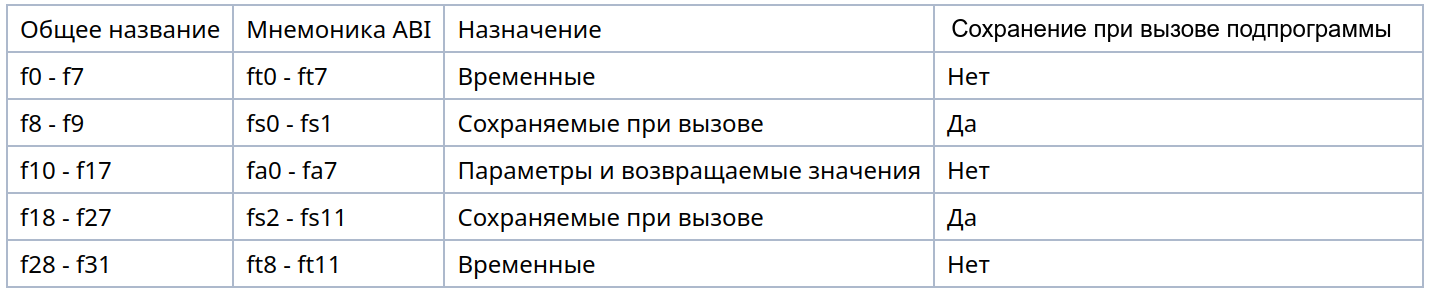
\includegraphics[width=1.0\textwidth]{img/fp-registers.png}
    \caption{Соглашения по использованию регистров с плавающей точкой}
    \label{fp-registers}
\end{figure}

Можно отметить, что в целом за счет отсутствия специализации, количество используемых регистров больше. Но при этом также заметить, что это расширение процессора. То есть, дополнительное устройство внутри кристалла. Следовательно, оно создается в случае более мощных процессоров и не присутствует в микроконтроллерах, которым оно не нужно из-за специфики их применения.

\subsection{Система команд математического сопроцессора}

\debate[Примечание]{Я разбил команды по группам на будущее. Возможно, что не совсем корректно и без перевода. Но думаю, что при формировании более сложной методы это можно будет повторно использовать.}

\subsubsection{Команды обработки данных арифметического сопроцессора}
Команды обработки данных арифметического сопроцессора представлены в таблице~\ref{table-fp-processor-calc}

\begin{table}[h]
    \caption{Команды обработки данных арифметического сопроцессора}
    \centering
    \begin{tabularx}{\textwidth}{|l|X|}
        \hline
        \textbf{Команда} & \textbf{Описание} \\
        %\hline  \multicolumn{3}{|c|}{\textbf{\textit{Арифметические}}} \\
        \hline \verb|fadd.d f1, f2, f3, dyn| & Floating ADD (64 bit): assigns f1 to f2 + f3 \\
        \hline \verb|fadd.s f1, f2, f3, dyn| & Floating ADD: assigns f1 to f2 + f3 \\
        \hline \verb|fdiv.d f1, f2, f3, dyn| & Floating DIVide (64 bit): assigns f1 to f2 / f3 \\
        \hline \verb|fdiv.s f1, f2, f3, dyn| & Floating DIVide: assigns f1 to f2 / f3 \\
        \hline \verb|fmul.d f1, f2, f3, dyn| & Floating MULtiply (64 bit): assigns f1 to f2 * f3 \\
        \hline \verb|fmul.s f1, f2, f3, dyn| & Floating MULtiply: assigns f1 to f2 * f3 \\
        \hline \verb|fsgnj.d f1, f2, f3| & Floating point sign injection (64 bit): replace the sign bit of f2 with the sign bit of f3 and assign it to f1 \\
        \hline \verb|fsgnj.s f1, f2, f3| & Floating point sign injection: replace the sign bit of f2 with the sign bit of f3 and assign it to f1 \\
        \hline \verb|fsgnjn.d f1, f2, f3| & Floating point sign injection (inverted 64 bit):  replace the sign bit of f2 with the opposite of sign bit of f3 and assign it to f1 \\
        \hline \verb|fsgnjn.s f1, f2, f3| & Floating point sign injection (inverted):  replace the sign bit of f2 with the opposite of sign bit of f3 and assign it to f1 \\
        \hline \verb|fsgnjx.d f1, f2, f3| & Floating point sign injection (xor 64 bit):  xor the sign bit of f2 with the sign bit of f3 and assign it to f1 \\
        \hline \verb|fsgnjx.s f1, f2, f3| & Floating point sign injection (xor):  xor the sign bit of f2 with the sign bit of f3 and assign it to f1 \\
        \hline \verb|fsub.d f1, f2, f3, dyn| & Floating SUBtract (64 bit): assigns f1 to f2 - f3 \\
        \hline \verb|fsub.s f1, f2, f3, dyn| & Floating SUBtract: assigns f1 to f2 - f3 \\
        \hline
    \end{tabularx}
    \label{table-fp-processor-calc}
\end{table}

\subsubsection{Команды пересылки данных арифметического сопроцессора}
Команды пересылки данных арифметического сопроцессора представлены в таблице~\ref{table-fp-processor-move}

\begin{table}[h]
    \caption{Команды пересылки данных арифметического сопроцессора}
    \centering
    \begin{tabularx}{\textwidth}{|l|X|}
        \hline
        \textbf{Команда} & \textbf{Описание} \\
        %\hline  \multicolumn{3}{|c|}{\textbf{\textit{Арифметические}}} \\
        \hline \verb|fld f1, -100(t1)| & Load a double from memory \\
        \hline \verb|flw f1, -100(t1)| & Load a float from memory \\
        \hline \verb|fmv.s.x f1, t1| & Move float: move bits representing a float from an integer register \\
        \hline \verb|fmv.x.s t1, f1| & Move float: move bits representing a float to an integer register \\
        \hline \verb|fsd f1, -100(t1)| & Store a double to memory \\
        \hline \verb|fsw f1, -100(t1)| & Store a float to memory \\
        \hline
    \end{tabularx}
    \label{table-fp-processor-move}
\end{table}

\subsubsection{Команды конвертации данных арифметического сопроцессора}
Команды конвертации данных арифметического сопроцессора представлены в таблице~\ref{table-fp-processor-convert}

\begin{table}[h]
    \caption{Команды конвертации данных арифметического сопроцессора}
    \centering
    \begin{tabularx}{\textwidth}{|l|X|}
        \hline
        \textbf{Команда} & \textbf{Описание} \\
        %\hline  \multicolumn{3}{|c|}{\textbf{\textit{Арифметические}}} \\
        \hline \verb|fcvt.d.s f1, f2, dyn| & Convert a float to a double: Assigned the value of f2 to f1 \\
        \hline \verb|fcvt.d.w f1, t1, dyn| & Convert double from integer: Assigns the value of t1 to f1 \\
        \hline \verb|fcvt.d.wu f1, t1, dyn| & Convert double from unsigned integer: Assigns the value of t1 to f1 \\
        \hline \verb|fcvt.s.d f1, f2, dyn| & Convert a double to a float: Assigned the value of f2 to f1 \\
        \hline \verb|fcvt.s.w f1, t1, dyn| & Convert float from integer: Assigns the value of t1 to f1 \\
        \hline \verb|fcvt.s.wu f1, t1, dyn| & Convert float from unsigned integer: Assigns the value of t1 to f1 \\
        \hline \verb|fcvt.w.d t1, f1, dyn| & Convert integer from double: Assigns the value of f1 (rounded) to t1 \\
        \hline \verb|fcvt.w.s t1, f1, dyn| & Convert integer from float: Assigns the value of f1 (rounded) to t1 \\
        \hline \verb|fcvt.wu.d t1, f1, dyn| & Convert unsinged integer from double: Assigns the value of f1 (rounded) to t1 \\
        \hline \verb|fcvt.wu.s t1, f1, dyn| & Convert unsinged integer from float: Assigns the value of f1 (rounded) to t1 \\
        \hline
    \end{tabularx}
    \label{table-fp-processor-convert}
\end{table}


Форматы команд математического сопроцессора совпадают с форматами \textbf{S} (запись в память, fs*), \textbf{I} (чтение из памяти, fl*) и \textbf{R} (вычисления).

Для хранения и передачи данных можно использовать слова, двойные слова, так как на уровне системы команд используется операционная однозначность (однозначность выполнения операций рассматривалась на лекциях). Поэтому мнемоника комнд пересылки использует обозначения <<word>> / <<double word>>: flw, fsw, fld, fsd, (а также *q и *h, если они реализованы в соответствующих стандартах расширений архитектуры).

Точность арифметических команд сопроцессора указывается суффиксом инструкции (s, d, q, h) который в ассемблере добавляется к коду операций, отделяясь от него точкой: \verb|fCMD.P|, где \verb|CMD| — мнемоника инструкции,
\verb|P| — точность.

Примеры команд \verb|CMD: add, sub, mul, div, sqrt, min, max|

\subsubsection{Вычисление полусуммы двух чисел}

Пример от Г.Курячего, демонстрирующий основные команды, пояснения есть в видео.

\begin{verbatim}
        .data
    a:      .float  123.456
    b:      .float  654.321
    _2:     .float  2
        .text
        flw     ft0 a t0
        flw     ft1 b t0
        flw     ft2 _2 t0
        fadd.s  ft3 ft2 ft1
        fdiv.s  fa0 ft3 ft2
        li      a7 2
        ecall
\end{verbatim}
При этом какие регистры и как используются определяется кодом операции. Информация об этих командах также имеется в системе помощи RARS. Переключение на сопроцессор осуществляет устройство управления по коду операции команды. Оно также определяе использование регистров с плавающей точкой совместно с целочисленными регистрами.

Пример раскрытия  команды \verb|flw| (рисунок~\ref{flw-example}). Представлен также в видео.

\begin{figure}[htbp]
    \centering
    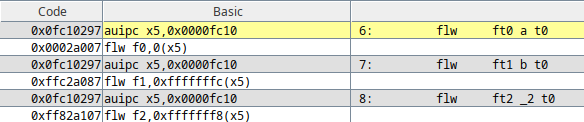
\includegraphics[width=1.0\textwidth]{img/flw-example.png}
    \caption{Раскрытие команды flw при ассемблировании}
    \label{flw-example}
\end{figure}
Также с данной программой можно пройтись пошагово. Тогда можно увидеть как меняются различные регистры. Обратить внимание на t0, используемый в данном случае для формирования базы адреса в памяти, чтобы обеспечить доступ для загрузки числа. А также отметить использование уже рассмотренной команды \verb|auipc| для формирования позиционно независимого кода. При этом можно обратить внимание, что 32-разрядные слова фиксируются в регистрах с плавающей точкой без указания старшей части, которая должна быть \textbf{NaN}.

\subsubsection{Команды арифметического сопроцессора, осуществляющие обработку сложных выражений}

Наряду с традиционными форматами команд в арифметический процессор добавлен новый тип команд \textbf{R4} (рисунок~\ref{fp-r4-type}), поддерживающих четыре операнда.

\begin{figure}[htbp]
    \centering
    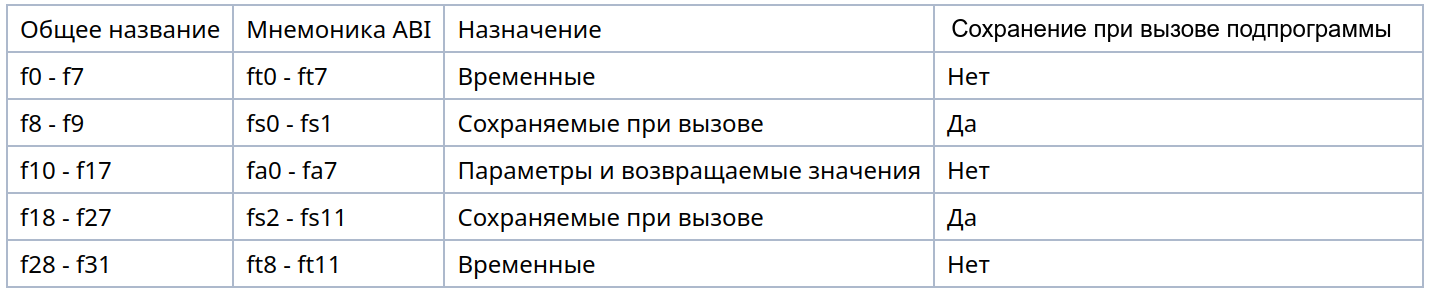
\includegraphics[width=1.0\textwidth]{img/fp-registers.png}
    \caption{Формат \textbf{R4}, используемый для поддержки составных операций}
    \label{fp-r4-type}
\end{figure}
Данные команды выполняют не элементарные действия а вычисления по более сложным выражениям с чередованием операций умножения, сложения, вычитания, смены знака. Эти команды представлены в таблице~\ref{table-fp-processor-complex}

\begin{table}[h]
    \caption{Команды арифметического сопроцессора, осуществляющие обработку сложных выражений}
    \centering
    \begin{tabularx}{\textwidth}{|l|X|}
        \hline
        \textbf{Команда} & \textbf{Описание} \\
        %\hline  \multicolumn{3}{|c|}{\textbf{\textit{Арифметические}}} \\
        \hline \verb|fmadd.d f1, f2, f3, f4, dyn| & Fused Multiply Add (64 bit): Assigns f2*f3+f4 to f1 \\
        \hline \verb|fmadd.s f1, f2, f3, f4, dyn| & Fused Multiply Add: Assigns f2*f3+f4 to f1 \\
        \hline \verb|fmsub.d f1, f2, f3, f4, dyn| & Fused Multiply Subatract: Assigns f2*f3-f4 to f1 \\
        \hline \verb|fmsub.s f1, f2, f3, f4, dyn| & Fused Multiply Subatract: Assigns f2*f3-f4 to f1 \\
        \hline \verb|fnmadd.d f1, f2, f3, f4, dyn| & Fused Negate Multiply Add (64 bit): Assigns -(f2*f3+f4) to f1 \\
        \hline \verb|fnmadd.s f1, f2, f3, f4, dyn| & Fused Negate Multiply Add: Assigns -(f2*f3+f4) to f1 \\
        \hline \verb|fnmsub.d f1, f2, f3, f4, dyn| & Fused Negated Multiply Subatract: Assigns -(f2*f3-f4) to f1 \\
        \hline \verb|fnmsub.s f1, f2, f3, f4, dyn| & Fused Negated Multiply Subatract: Assigns -(f2*f3-f4) to f1 \\
        \hline \verb|fmax.d f1, f2, f3| & Floating MAXimum (64 bit): assigns f1 to the larger of f1 and f3 \\
        \hline \verb|fmax.s f1, f2, f3| & Floating MAXimum: assigns f1 to the larger of f1 and f3 \\
        \hline \verb|fmin.d f1, f2, f3| & Floating MINimum (64 bit): assigns f1 to the smaller of f1 and f3 \\
        \hline \verb|fmin.s f1, f2, f3| & Floating MINimum: assigns f1 to the smaller of f1 and f3 \\
        \hline \verb|fsqrt.d f1, f2, dyn| & Floating SQuare RooT (64 bit): Assigns f1 to the square root of f2 \\
        \hline \verb|fsqrt.s f1, f2, dyn| & Floating SQuare RooT: Assigns f1 to the square root of f2 \\
        \hline
    \end{tabularx}
    \label{table-fp-processor-complex}
\end{table}

\subsection{Обмен между регистрами с плавающей точкой и целочисленными регистрами}

Можно обмениваться не с памятью, а с регистрами общего назначения. В мнемонике используются два суффикса:

Перемещать машинное слово из одного регистра в другой умеет центральный процессор: \verb|fmv.s.x| и \verb|fmv.x.s| (для двойной точности такой инструкции нет, так как процессор манипулирует только 32-х разрядными словами). Целое число при этом не преобразуется.

Но преобразовывать из вещественного формата в целый и обратно (а также из двойного в одинарный и обратно) может только FPU: \verb|fcvt.d.s| \verb|fcvt.s.d|, \verb|fcvt.P.w[u]| и \verb|fcvt.w[u].P|.

Пример вычисления функции $(x-1)^2$. Расчет с использованием приведения формулы к виду: $x^2-2x+1$.
\begin{verbatim}
        .data
    x:      .double 12.34
        .text
    li              t2 2
    fcvt.d.w        ft2 t2                  # ft2 = 2.0
    li              t1 1
    fcvt.d.w        ft1 t1                  # ft1 = 1.0
    fld             ft0 x t0                # ft0 = x
    fnmsub.d        ft3 ft2 ft0 ft1         # ft3 = -(2 * x) + 1
    fmadd.d         fa0 ft0 ft0 ft3         # fa0 = x * x + ft3
    li              a7 3                    # Вывод числа двойной точности
    ecall
\end{verbatim}

Перемещение между f-регистрами: \verb|fmv f1 f2| --- в действительности это псевдоинструкция на базе инструкции расширения знака \verb|fsgnj.P|.

Во многих архитектурах (в частности, MIPS) недооценили важность и частоту операции <<смены знака по образцу>>, а вычислительно эта операция непростая, особенно для вещественных чисел. Поэтому в RISC-V есть специальная операция: взять знак из \verb|fA|, а мантиссу и порядок из \verb|fB|, и всё это положить в \verb|fC|.

Tогда fmv раcrрывается так:

\verb|0x00400028  0x222100d3  fsgnj.d f1,f2,f2     13     fmv.d   ft1 ft2|

\subsection{Команды сравнения}

f{eq|lt|le}/P x1 f1 f2 — записывает 0 или 1 в x1

Остальные сравнения --- псевдоинструкции

\debate[TODO]{При дальнейшем оформлении сюда стоит перетащить команды из таблицы.}

\section{Псевдоинструкции}

\debate[Примечание]{Вопрос: где о них говорить? В ходе пояснения основных групп команд или отдельно? На выбор, наверное.}

Как и в случае с командами основного процессора, при программировании арифметического процессора также используются псевдоинструкции (псевдокоманды), повышающие гибкость в разработке программ. Они затрагивают практически весь спектр команд с плавающей точкой и ниже представлены разнесенными в различные подгруппы.

\subsection{Псевдоинструкции для обработки данных}

Как и соответствующие команды, команды обработки данных осуществляют различные функциональные преобразования. Они представлены в таблице~\ref{table-fp-pseudo-calc}.

\begin{table}[h]
    \caption{Псевдокоманды обработки данных}
    \centering
    \begin{tabularx}{\textwidth}{|l|X|}
        \hline
        \textbf{Команда} & \textbf{Описание} \\
        \hline \verb|fabs.d f1, f2| & Set f1 to the absolute value of f2 (64 bit) \\
        \hline \verb|fabs.s f1, f2| & Set f1 to the absolute value of f2 \\
        \hline \verb|fadd.d f1, f2, f3| & Floating ADD (64 bit): assigns f1 to f2 + f3 \\
        \hline \verb|fadd.s f1, f2, f3| & Floating ADD: assigns f1 to f2 + f3 \\
        \hline \verb|fdiv.d f1, f2, f3| & Floating DIVide (64 bit): assigns f1 to f2 / f3 \\
        \hline \verb|fdiv.s f1, f2, f3| & Floating DIVide: assigns f1 to f2 / f3 \\
        \hline \verb|fmadd.d f1, f2, f3, f4| & Fused Multiply Add (64 bit): Assigns f2*f3+f4 to f1 \\
        \hline \verb|fmadd.s f1, f2, f3, f4| & Fused Multiply Add: Assigns f2*f3+f4 to f1 \\
        \hline \verb|fmsub.d f1, f2, f3, f4| & Fused Multiply Subatract (64 bit): Assigns f2*f3-f4 to f1 \\
        \hline \verb|fmsub.s   f1, f2, f3, f4| & Fused Multiply Subatract: Assigns f2*f3-f4 to f1 \\
        \hline \verb|fmul.d    f1, f2, f3| & Floating MULtiply (64 bit): assigns f1 to f2 * f3 \\
        \hline \verb|fmul.s    f1, f2, f3| & Floating MULtiply: assigns f1 to f2 * f3 \\
        \hline \verb|fneg.d f1, f2| & Set f1 to the negation of f2 (64 bit) \\
        \hline \verb|fneg.s f1, f2| & Set f1 to the negation of f2 \\
        \hline \verb|fnmadd.d  f1, f2, f3, f4| & Fused Negate Multiply Add (64 bit): Assigns -(f2*f3+f4) to f1 \\
        \hline \verb|fnmadd.s  f1, f2, f3, f4| & Fused Negate Multiply Add: Assigns -(f2*f3+f4) to f1 \\
        \hline \verb|fnmsub.d  f1, f2, f3, f4| &  \\
        \hline \verb|| & Fused Negated Multiply Subatract (64 bit): Assigns -(f2*f3-f4) to f1 \\
        \hline \verb|fnmsub.s  f1, f2, f3, f4| & Fused Negated Multiply Subatract: Assigns -(f2*f3-f4) to f1 \\
        \hline \verb|fsqrt.d   f1, f2| & Floating SQuare RooT (64 bit): Assigns f1 to the square root of f2 \\
        \hline \verb|fsqrt.s   f1, f2| & Floating SQuare RooT: Assigns f1 to the square root of f2 \\
        \hline \verb|fsub.d    f1, f2, f3| & Floating SUBtract (64 bit): assigns f1 to f2 - f3 \\
        \hline \verb|fsub.s    f1, f2, f3| & Floating SUBtract: assigns f1 to f2 - f3 \\
        \hline
    \end{tabularx}
    \label{table-fp-pseudo-calc}
\end{table}

\subsection{Псевдоинструкции пересылки, загрузки и сохранения данных}

Псевдокоманды, обеспечивающие пересылку данных между различными регистрами и областями памяти представлены в таблице~\ref{table-fp-pseudo-mov-load-store}. Они расширяют возможности основных команд пересылки данных, обеспечивая программиста более компактными псевдонимами.

\begin{table}[h]
    \caption{Псевдокоманды пересылки, загрузки, сохранения}
    \centering
    \begin{tabularx}{\textwidth}{|l|X|}
        \hline
        \textbf{Команда} & \textbf{Описание} \\
        \hline \texttt{fld f1,\%lo(label)(t2)} & Load from Address \\
        \hline \verb|fld f1,(t2)| & Load Word: Set f1 to 64-bit value from effective memory word address \\
        \hline \verb|fld f1,-100| & Load Word: Set f1 to 64-bit value from effective memory word address \\
        \hline \verb|fld f1,10000000,t3| & Load Word: Set f1 to 64-bit value from effective memory word address using t3 as a temporary \\
        \hline \verb|fld f1,label, t3| & Load Word: Set f1 to 64-bit value from effective memory word address using t3 as a temporary \\
        \hline \texttt{flw f1,\%lo(label)(t2)} & Load from Address \\
        \hline \verb|flw f1,(t2)| & Load Word Coprocessor 1 : Set f1 to 32-bit value from effective memory word address \\
        \hline \verb|flw f1,-100| & Load Word Coprocessor 1 : Set f1 to 32-bit value from effective memory word address \\
        \hline \verb|flw f1,10000000,t3| & Load Word Coprocessor 1 : Set f1 to 32-bit value from effective memory word address using t3 as a temporary \\
        \hline \verb|flw f1,label, t3| & Load Word Coprocessor 1 : Set f1 to 32-bit value from effective memory word address using t3 as a temporary \\
        \hline \verb|fmv.d  f1, f2| & Move the value of f2 to f1 (64 bit) \\
        \hline \verb|fmv.s  f1, f2| & Move the value of f2 to f1 \\
        \hline \verb|fmv.w.x f1, t1| & Move float (New mnemonic): move bits representing a float from an integer register \\
        \hline \verb|fmv.x.w t1, f1| & Move float (New mnemonic): move bits representing a float to an integer register \\
        \hline \verb|fsd f1,(t2)| & Store Word: Store 64-bit value from f1 to effective memory word address \\
        \hline \verb|fsd f1,-100 | & Store Word: Store 64-bit value from f1 to effective memory word address \\
        \hline \verb|fsd f1,10000000,t3| & Store Word: Store 64-bit value from f1 to effective memory word address using t3 as a temporary \\
        \hline \verb|fsd f1,label, t3| &  \\
        \hline \verb|| & Store Word: Store 64-bit value from f1 to effective memory word address using t3 as a temporary \\
        \hline \verb|fsw f1,(t2)| & Store Word Coprocessor 1 : Store 32-bit value from f1 to effective memory word address \\
        \hline \verb|fsw f1,-100| & Store Word Coprocessor 1 : Store 32-bit value from f1 to effective memory word address \\
        \hline \verb|fsw f1,10000000,t3| & Store Word Coprocessor 1 : Store 32-bit value from f1 to effective memory word address using t3 as a temporary \\
        \hline \verb|fsw f1,label, t3| & Store Word Coprocessor 1 : Store 32-bit value from f1 to effective memory word address using t3 as a temporary \\
        \hline
    \end{tabularx}
    \label{table-fp-pseudo-mov-load-store}
\end{table}

\subsection{Псевдоинструкции сравнения}

Псевдокоманды сравнения представлены в таблице~\ref{table-fp-pseudo-cmp}. Через уже существующие команды реализованы псевдокоманды, задающие отношения больше, а также больше или равно.

\begin{table}[h]
    \caption{Псевдокоманды сравнения}
    \centering
    \begin{tabularx}{\textwidth}{|l|X|}
        \hline
        \textbf{Команда} & \textbf{Описание} \\
        \hline \verb|fge.d t1, f2, f3| & Floating Greater Than or Equal (64 bit): if f2 >= f3, set t1 to 1, else set t1 to 0 \\
        \hline \verb|fge.s t1, f2, f3| & Floating Greater Than or Equal: if f2 >= f3, set t1 to 1, else set t1 to 0 \\
        \hline \verb|fgt.d t1, f2, f3| & Floating Greater Than (64 bit): if f2 > f3, set t1 to 1, else set t1 to 0 \\
        \hline \verb|fgt.s t1, f2, f3| & Floating Greater Than: if f2 > f3, set t1 to 1, else set t1 to 0 \\
        \hline
    \end{tabularx}
    \label{table-fp-pseudo-cmp}
\end{table}

\subsection{Псевдоинструкции конвертации данных}

Данный вид псевдоинструкций осуществляет трансформацию между различными форматами данных. Соответствующие псевдоинструкции представлены в таблице~\ref{table-fp-pseudo-convert}.

\begin{table}[h]
    \caption{Псевдокоманды преобразования данных}
    \centering
    \begin{tabularx}{\textwidth}{|l|X|}
        \hline
        \textbf{Команда} & \textbf{Описание} \\
        \hline \verb|fcvt.d.s f1, f2| & Convert float to double: Assigned the value of f2 to f1 \\
        \hline \verb|fcvt.d.w  f1, t1| & Convert double from signed integer: Assigns the value of t1 to f1 \\
        \hline \verb|fcvt.d.wu f1, t1| & Convert double from unsigned integer: Assigns the value of t1 to f1 \\
        \hline \verb|fcvt.s.d f1, f2| & Convert double to float: Assigned the value of f2 to f1 \\
        \hline \verb|fcvt.s.w  f1, t1| & Convert float from signed integer: Assigns the value of t1 to f1 \\
        \hline \verb|fcvt.s.wu f1, t1| & Convert float from unsigned integer: Assigns the value of t1 to f1 \\
        \hline \verb|fcvt.w.d  t1, f1| & Convert signed integer from double: Assigns the value of f1 (rounded) to t1 \\
        \hline \verb|fcvt.w.s  t1, f1| & Convert signed integer from float: Assigns the value of f1 (rounded) to t1 \\
        \hline \verb|fcvt.wu.d t1, f1| & Convert unsigned integer from double: Assigns the value of f1 (rounded) to t1 \\
        \hline \verb|fcvt.wu.s t1, f1| & Convert unsigned integer from float: Assigns the value of f1 (rounded) to t1 \\
        \hline
    \end{tabularx}
    \label{table-fp-pseudo-convert}
\end{table}


% --- Семинар 09. Ввод--вывод данных. Поллинг. Программирование ввода--вывода ---
\chapter[Арифметика с плавающей точкой. Продолжение]{Семинар 09. Математический сопроцессор. Арифметика с плавающей точкой. Продолжение }

Продолжение темы по арифметическому сопроцессору. В данном случае искусственное разделение темы по занятиям. Часть вопросов рассмотрено в продолжении рассматрвается:

На занятии предполагается рассмотреть следующие темы, связанные с управлением вычислениями в арифметическом сопроцессоре:
\begin{enumerate}
    \item Сравнение данных с плавающей точкой.
    \item Команды классификации
    \item Блок управляющих регистров
    \item Условные операторы и fcsr
    \item Проверка на потерю точности.
\end{enumerate}

\section{Сравнение данных с плавающей точкой}

\subsubsection{Команды сравнения и анализа}
Команды сравнения и анализа представлены в таблице~\ref{table-fp-processor-cmp}

\begin{table}[h]
    \caption{Команды сравнения и анализа}
    \centering
    \begin{tabularx}{\textwidth}{|l|X|}
        \hline
        \textbf{Команда} & \textbf{Описание} \\
        %\hline  \multicolumn{3}{|c|}{\textbf{\textit{Арифметические}}} \\
        \hline \verb|fclass.d t1, f1| & Classify a floating point number (64 bit) \\
        \hline \verb|fclass.s t1, f1| & Classify a floating point number \\
        \hline \verb|feq.d t1, f1, f2| & Floating EQuals (64 bit): if f1 = f2, set t1 to 1, else set t1 to 0 \\
        \hline \verb|feq.s t1, f1, f2| & Floating EQuals: if f1 = f2, set t1 to 1, else set t1 to 0 \\
        \hline \verb|fle.d t1, f1, f2| & Floating Less than or Equals (64 bit): if f1 <= f2, set t1 to 1, else set t1 to 0 \\
        \hline \verb|fle.s t1, f1, f2| & Floating Less than or Equals: if f1 <= f2, set t1 to 1, else set t1 to 0 \\
        \hline \verb|flt.d t1, f1, f2| & Floating Less Than (64 bit): if f1 < f2, set t1 to 1, else set t1 to 0 \\
        \hline \verb|flt.s t1, f1, f2| & Floating Less Than: if f1 < f2, set t1 to 1, else set t1 to 0 \\
        \hline
    \end{tabularx}
    \label{table-fp-processor-cmp}
\end{table}

\section{Команды классификации}

Инструкция \verb|fclass.(s/d) t1, f1| проверяет значение в регистре чисел с плавающей точкой \verb|f1| и записывает в целочисленный регистр \verb|t1| 10-битную маску, указывающую класс числа с плавающей запятой. Формат маски описан в таблице~\ref{table-fclass-mask}. Соответствующий бит в t1 будет установлен, если свойство истинно, и очищен в противном случае. Все остальные биты в \verb|t1| очищаются. При этом в \verb|t1| \textbf{будет установлен только один бит}. \verb|fclass| не устанавливает флаги исключений с плавающей запятой.

\begin{table}[h]
    \caption{Биты, устанавливаемые командами классификации}
    \centering
    \begin{tabularx}{\textwidth}{|c|X|}
        \hline
        \textbf{Установленный бит} & \textbf{Свойства числа с плавающей точкой} \\
        %\hline  \multicolumn{3}{|c|}{\textbf{\textit{Арифметические}}} \\
        \hline \verb|0 (0x001)| & f1 --- это -$\infty$  \\
        \hline \verb|1 (0x002)| & f1 --- это отрицительное нормализованное число \\
        \hline \verb|2 (0x004)| & f1 --- это отрицительное денормализованное число \\
        \hline \verb|3 (0x008)| & f1 --- это -0 \\
        \hline \verb|4 (0x010)| & f1 --- это +0 \\
        \hline \verb|5 (0x020)| & f1 --- это положительное денормализованное число \\
        \hline \verb|6 (0x040)| & f1 --- это положительное нормализованное число \\
        \hline \verb|7 (0x080)| & f1 --- это +$\infty$ \\
        \hline \verb|8 (0x100)| & f1 --- это сигнализирующий NaN \\
        \hline \verb|9 (0x200)| & f1 --- это тихий NaN \\
        \hline
    \end{tabularx}
    \label{table-fclass-mask}
\end{table}

Можно отметить, что в отличие от целочисленной арифметики проверка результатов вычислений с плавающей точкой может играть важное значение для получения достоверных решений. Например, возможно перемножение чисел, сильно отличающихся друг от друга, что ведет к накоплению ошибки вплоть до переполнения или исчесзновения порядка. Поэтому ввод в спецпроцессор дополнительных команд контроля и классификации, обеспечивающих подобные проверки для принятия решений и управления, оправдан.

Для демонстрации я создал макрос \verb|macro-is-class.mac|, который выводит информацию об этих проверках (лежит в каталоге \verb|is-class| вместе с тестовой программой). Тестовый код можно расширить, добавив туда различные варианты чисел с плавающей точкой. Для получения крайних значений можно использовать либо пересылки данных посредством их подготовки в целочисленных регистрах, либо готовить их с использованием диалогового окна (для 32-х разрядных чисел).

\section{Блок управляющих регистров (общее представление)}

Блок управляющих регистров (БУР) --- Control and Status Register (CSR). Более подробно будет рассматриваться при изучении новых свойств. Пока кратко применительно к арифметическому сопроцессору.

RISC-V определяет отдельное адресное пространство из 4096 регистров управления и состояния, связанных с каждым портом. Регистры образуют 4K (12 битов) пространство управляющих счётчиков, флагов, масок и прочего. Имеется набор инструкций CSR, которые работают с блоком. Все инструкции CSR атомарно читают-изменяют-записывают один регистр блока, спецификатор регистра которого закодирован в 12-битном поле csr инструкции, хранящемся в битах 31–20. Это атомарные R/W инструкции типа I.

В RARS часть используемых регистров отображается во вкладке <<\textbf{Control and Status}>>.

Команды для работы с блоком управляющих регистров представлены в тиблице~\ref{table-csr-commands}.
Все инструкции CSR атомарно читают--изменяют--записывают один CSR, спецификатор CSR которого закодирован в 12-битном поле csr инструкции, хранящемся в битах 31–20. Инструкции с непосредственным операндом используют 5-битную расширенную нулем непосредственную информацию, закодированную в поле rs1.

\begin{table}[h]
    \caption{Команды для работы с регистром блока управляющих регистров}
    \centering
    \begin{tabularx}{\textwidth}{|l|X|}
        \hline
        \textbf{Команда} & \textbf{Описание} \\
        \hline \verb|csrrc t0, fcsr, t1| & Atomic Read/Clear CSR: read from the CSR into t0 and clear bits of the CSR according to t1 \\
        \hline \verb|csrrci t0, fcsr, 10| & Atomic Read/Clear CSR Immediate: read from the CSR into t0 and clear bits of the CSR according to a constant \\
        \hline \verb|csrrs t0, fcsr, t1| & Atomic Read/Set CSR: read from the CSR into t0 and logical or t1 into the CSR \\
        \hline \verb|csrrsi t0, fcsr, 10| & Atomic Read/Set CSR Immediate: read from the CSR into t0 and logical or a constant into the CSR \\
        \hline \verb|csrrw t0, fcsr, t1| & Atomic Read/Write CSR: read from the CSR into t0 and write t1 into the CSR \\
        \hline \verb|csrrwi t0, fcsr, 10| & Atomic Read/Write CSR Immediate: read from the CSR into t0 and write a constant into the CSR \\
        \hline
    \end{tabularx}
    \label{table-csr-commands}
\end{table}
То есть, основная идея практически всех команд заключается в сохранении читаемого состояния и в различных вариантов установки нового состояния одного из регистров.

\subsection{Регистр fcsr (0x003)}

Регистр \verb|fcsr| имеет следующие поля:

\begin{itemize}
    \item 5 бит --- флаги
    \begin{itemize}
        \item NX потеря точности
        \item UF сверхмалое число
        \item OF переполнение
        \item DZ деление на 0
        \item NV недопустимая операция
    \end{itemize}
    \item 3 бита --- тип округления
    \begin{itemize}
        \item RNE ближайшее, лучше чётное
        \item RTZ ближайшее к нулю
        \item RDN ближайшее к -$\infty$
        \item RUP ближайшее к +$\infty$
        \item RMM ближайшее, лучше с большим модулем
        \item ...
        \item ...
        \item DYN не менять установленное по умолчанию (используется в инструкциях явного округления)
    \end{itemize}
\end{itemize}
Для работы с регистром \verb|fcsr| используются псевдоинструкции типа \verb|f[sr]csr|. В RARS, видимо для удобства,  в отдельные регистры выделены регистры \verb|frm| и \verb|fflags|, хотя это на самом деле поля \verb|fcsr|. С \verb|fflags| используется отдельная псевдоинструкция \verb|frflags|, а \verb|frm| используется инструкция \verb|fsrm|. Соответствующие псевдоинструкции представлены в таблице~\ref{table-fcsr-pseudo}.

\begin{table}[h]
    \caption{Псевдокоманды для работы с регистром \texttt{fcsr}}
    \centering
    \begin{tabularx}{\textwidth}{|l|X|}
        \hline
        \textbf{Команда} & \textbf{Описание} \\
        \hline \verb|frcsr t1| & Read FP control/status register \\
        \hline \verb|frflags t1| & Read FP exception flags \\
        \hline \verb|frrm t1| & Read FP rounding mode \\
        \hline \verb|frsr t1| & Alias for frcsr t1 \\
        \hline \verb|fscsr t1, t2| & Swap FP control/status register \\
        \hline \verb|fscsr t1| & Write FP control/status register \\
        \hline \verb|fsflags t1| & Write FP exception flags \\
        \hline \verb|fsflags t1, t2| & Swap FP exception flags \\
        \hline \verb|fsrm t1| & Write FP rounding mode \\
        \hline \verb|fsrm t1, t2| & Swap FP rounding mode \\
        \hline \verb|fssr t1| & Alias for fscsr t1 \\
        \hline \verb|fssr t1, t2| & Alias for fscsr t1, t2 \\
        \hline
    \end{tabularx}
    \label{table-fcsr-pseudo}
\end{table}

В примере \verb|round-up| приведено использование округления различными способами с использованием псевдокоманды  \verb|fsrm|:
\begin{itemize}
    \item по умолчанию;
    \item в сторону 0 (явно);
    \item в сторону минус бесконечности.
\end{itemize}

\begin{verbatim}
    .data
    numb:   .float  7.5

    .text
    flw     ft0 numb t0
    fcvt.w.s a0 ft0         # По умолчанию RNE (ближайшее, чётное) = 8
    jal     outn
    fcvt.w.s a0 ft0 rtz     # Ближайшее к 0 = 7
    jal     outn
    li      t0 2            # RDN — ближайшее к -бесконечности
    fsrm    t0
    fcvt.w.s a0 ft0         # теперь по умолчанию RDN = 7
    jal     outn
    fcvt.w.s a0 ft0 dyn     # Не менять установленное по умолчанию = 7
    jal     outn
    fcvt.w.s a0 ft0 rne     # RNE (ближайшее, чётное) = 8
    jal     outn

    li      a7 10
    ecall

    outn:   li      a7 1
    ecall
    li      a0 '\n'
    li      a7 11
    ecall
    ret
\end{verbatim}

\debate[Примечание]{Я расширил пример. Здесь можно выдать задание потренироваться на подстановку различных чисел: отрицательных с дробной частью больше и меньше 0.5 и т.д.}

\section{Условные операторы и fcsr}

Наряду с осуществление непосредственных сравнений, арифметический сопроцессор отображает своё состояние в управляющем регистре \verb|fcsr|, который входит в блок управляющих регистров \textbf{CSR (Control and Status Register)}. Использование дополнительных регистров флагов и состояний в спецпроцессорах оправдано, так как существует необходимость в выполнении быстрых проверок сразу же после выполнения их инструкций.

Варианты организации условных переходов:
\begin{itemize}
    \item использование инструкций \verb|fCMP.P / fclas.P| с последующим переходом по содержимому целочисленного (X) регистра (0 / не 0);
    \item использование инструкций \verb|fcsr*/frflags| с чтением всех флагов в целочисленный регистр, выделением конкретного флага инструкцией, например, \verb|andi| и условный переход по содержимому целочисленного (X) регистра (0 / не 0).
\end{itemize}
В любом случае условный переход неатомарен.

Использование условных переходов на примере определения того, являются ли три отрезка сторонами треугольника (\verb|is-float-triangle.s|). Используются команды непосредственного сравнения на неравенство с последующим объединением результатов сравнения по \textbf{И} (все неравенства должны быть истинными).

\begin{verbatim}
    .data
    yes:    .asciz  "It is a triangle\n"
    no:     .asciz  "It is not a triangle\n"
    .text
    jal     input
    fmv.d   fs2 fa0
    jal     input
    fmv.d   fs1 fa0
    jal     input
    fmv.d   fa1 fs1
    fmv.d   fa2 fs2
    jal     check
    bnez    a0 true
    la      a0 no
    b       output
    true:
    la      a0 yes
    output: li      a7 4
    ecall
    li      a7 10
    ecall

    .data
    prompt: .ascii  "Enter triangle side: "
    .text
    input:
    la      a0 prompt
    li      a7 4
    ecall
    li      a7 7
    ecall
    ret

    check:  fadd.d  ft0 fa1 fa2
    flt.d   t0 fa0 ft0
    fadd.d  ft1 fa2 fa0
    flt.d   t1 fa1 ft1
    fadd.d  ft2 fa1 fa0
    flt.d   t2 fa2 ft2
    and     a0 t0 t1
    and     a0 a0 t2
    ret
\end{verbatim}

Следующий пример демонстрирует анализ на потерю точности, возможную в вычислительных задачах (\verb|precision.s|). Вычисляется выражение \verb|(a + b) / c|.

\begin{verbatim}
    .include "macro-common.mac"
    .data
    Exact:  .asciz  " - это точное решение!\n"
    Inex:   .asciz  " - результат неточный (с округлением).\n"

    .text
    print_str ("Считаем по формуле: (a + b) / c\n")
    print_str ("a = ")
    li      a7 6
    ecall
    fmv.s   fs0 fa0         # A
    print_str ("b = ")
    li      a7 6
    ecall
    fmv.s   fs1 fa0         # B
    print_str ("c = ")
    li      a7 6
    ecall
    fmv.s   fs2 fa0         # C

    fadd.s  ft0 fs0 fs1
    frflags t0              # Флаги FPU
    andi    t0 t0 1         # Потеря точности?
    fdiv.s  fa0 ft0 fs2
    frflags t1              # Флаги FPU
    andi    t1 t1 1         # Потеря точности?
    or      s1 t0 t1        # ...хотя бы раз
    print_str ("Result = ")
    li      a7 2
    ecall
    la      a0 Inex
    bnez    s1 out
    la      a0 Exact

    out:    li      a7 4
    ecall
    li      a7 10
    ecall
\end{verbatim}

\debate[Примечание]{Для большей наглядности я подключил макробиблиотеку для вывода вспомогательных сообщений.}

\debate[Примечание]{Думаю, что по объему где-то примерно здесь (может чуть раньше или позже) будет конец второго семинара по теме. Но это можно сдвигать и обсуждать полученные реальные ситуации.}


% --- Семинар 10. Таймер. Прерывания по таймеру ---
\chapter[Арифметика с плавающей точкой. Примеры]{Семинар 10. Математический сопроцессор. Арифметика с плавающей точкой. Окончание}

Завершение темы сопровождается рядом примеров. Возможно их не так много. Но пока в голову больше не лезет. В качестве дополнения можно рассмотреть дополнительное оформление в виде подпрограмм и макросов, обеспечивающих повышение юзабилити.

На занятии предполагается рассмотреть следующие примеры:
\begin{enumerate}
    \item Предварительная проверка числа перед выполнением вычислений на примере вычисления квадратного корня.
    \item Вычисление площади треугольника по формуле Герона.
    \item Вычисление числа $e$ с заданной точностью.
\end{enumerate}


\section{Примеры вычислений с плавающей точкой}

Специфической особенностью арифметики с плавающей точкой является отсутствие точных проверок чисел на равенство. Помимо этого часто различные вычисления осуществляются приближенно с заданной точностью.

\subsection{Предварительная проверка числа перед выполнением вычислений на примере вычисления квадратного корня}

Ниже представлено (из Г. Курячего) вычисление квадратного корня из целого числа, с предварительной проверкой его на положительное значение уже в регистре арифметического сопроцессора:

\begin{verbatim}
    li      a7 5
    ecall                   # Ввод целого
    fcvt.s.w ft1 a0         # Преобразование в вещественное
    fmv.s.x ft0 zero        # 0 не надо преобразовывать!
    flt.s   t0 ft1 ft0      # t0 = ft1 < 0 ?
    fmv.s   fa0 ft0         # результат пока 0...
    bnez    t0 negat        # ... и останется 0, если число отрицательное
    fsqrt.s fa0 ft1         # вычислим корень
    negat:  li      a7 2            # выведем результат
    ecall
    li      a7 10
    ecall
\end{verbatim}

\debate[Примечание]{Код простой. Поэтому со вспомогательными сообщениями решил не мудрить.}

\subsection{Вычисление площади треугольника по формуле Герона}

В примере рассматривается простое решение, связанное с вычислением плошади треугольника по формуле:
$S = \sqrt{p*(p-a)*(p-b)*(p-c)}$
где
$a, b, c$ - стороны треугольника,
$p = (a+b+c)/2$.

Простая программа (triangle-area) выглядит следующим образом:
\begin{verbatim}
    .data
    yes:    .asciz  "It is a triangle\n"
    no:     .asciz  "It is not a triangle\n"
    area:   .asciz  "Area = \n"
    .text
    # Последовательный ввод трех сторон
    jal     input
    fmv.s   fs2 fa0
    jal     input
    fmv.s   fs1 fa0
    jal     input
    fmv.s   fa1 fs1
    fmv.s   fa2 fs2

    jal     check      # Вызов проверки на треугольник

    # Это не треугольник
    bnez    a0 true
    la      a0 no
    li      a7 4
    ecall
    b       exit

    # Это треугольник.
    true:   la      a0 yes
    li      a7 4
    ecall
    jal     geron   # Вычисление площади
    li		a7 2	# Вывод площади
    ecall
    exit:
    li      a7 10
    ecall

    # Ввод стороны треугольника
    .data
    prompt: .ascii  "Enter triangle side: "
    .text
    input:  la      a0 prompt
    li      a7 4
    ecall
    li      a7 6
    ecall
    ret

    # Проверка, что это стороны треугольника
    check:  fadd.s  ft0 fa1 fa2
    flt.s   t0 fa0 ft0
    fadd.s  ft1 fa2 fa0
    flt.s   t1 fa1 ft1
    fadd.s  ft2 fa1 fa0
    flt.s   t2 fa2 ft2
    and     a0 t0 t1
    and     a0 a0 t2
    ret

    # Вычисление площади по формуле Герона
    # Стороны остались в регистрах - параметрах
    .data
    double_two: .float 2.0
    .text
    geron:
    # Вычисления полупериметра
    fadd.s 	ft0 fa0 fa1
    fadd.s 	ft0 ft0 fa2
    flw		ft2 double_two t0
    fdiv.s 	ft0 ft0 ft2
    # Вычисление разностей
    fsub.s	ft3 ft0 fa0
    fsub.s	ft4 ft0 fa1
    fsub.s	ft5 ft0 fa2
    # Их перемножение
    fmul.s	ft1 ft3 ft4
    fmul.s	ft1 ft1 ft5
    fmul.s	ft1 ft1 ft0
    # Получение площади
    fsqrt.s	fa0 ft1
    ret
\end{verbatim}


\subsection{Вычисление числа $e$ с заданной точностью}

Пример (\verb|exp.s|) такой же как и у Курячего. Только взят из другого источника. Поэтому комментарии на английском. Вычисляет число $e$ по формуле:

$\exp = 1/n! + 1/(n-1)! + ...$

Точность задается формулой:

$\epsilon = 1/(10 ** k))$

Добавил подсказку для ввода  данных с использованием библиотеки макроопределений.

\begin{verbatim}
    #
    # Example: calculates e as an infinite sum: 1/n! + 1/(n-1)! + ...
    #          with the specified precision epsilon = 1/(10 ** k))
    #
    .include "common.mac"
    .data
    one:
    .double 1
    ten:
    .double 10

    .text
    main:
    fld     f2, one, t0   # 1
    fsub.d  f4, f4, f4    # n = 0
    fmv.d   f6, f2        # n!
    fmv.d   f8, f2        # here will be e
    fld     f10, ten, t0  # here will be epsilon
    fmv.d   f0, f2        # decimal length k

    print_str("Введите число точных разрядов: ")
    read_int_a0
    enext:
    blez    a0, edone     # 10 ** (k+1)
    fmul.d  f0, f0, f10
    addi    a0, a0, -1
    j       enext
    edone:
    fdiv.d  f10, f2, f0   # epsilon

    loop:
    fadd.d  f4, f4, f2    # n = n+1
    fmul.d  f6, f6, f4    # n! = (n-1)! * n
    fdiv.d  f0, f2, f6    # next summand
    fadd.d  f8, f8, f0
    flt.d   t0, f0, f10   # next summand < epsilon
    beqz    t0, loop

    li      a7, 3         # output a double
    fmv.d   fa0, f8
    ecall
\end{verbatim}

\section{Домашнее задание}

\debate[Примечание]{\textbf{\textit{Домашнее задание на арифметику с плавающей точкой не выдаем. Текст оставляю на будущее (на всякий случай, чтобы не вспоминать). Компенсируется индивидуальным заданием по этой теме.}}}

\textbf{До 8 баллов}

Написать программу, осуществляющую вычисление корня квадратного из положительного числа с заданной точностью, используя для этого соответствующую итерационную формулу. В качестве исходных данных вводятся  исходное действительное число и точность вычислений, задаваемая также действительным числом. Вычисление корня оформить как отдельную подпрограмму, принимающую значение аргумента и точность, которая возвращает в качестве результата полученную величину квадратного корня. Основная программа осуществляет ввод исходного числа и точности с консоли с проверкой на корректные значения, а также вывод результата.

\textbf{Опционально до +2 баллов}

Обернуть ввод исходных данных и их проверку, вывод результата вычислений, вызов подпрограммы вычисления квадратного корня в отдельные макроопределения. Эти макроопределения оформить в отдельном файле, подключаемом к основной программе вместо описания в ней глобальных точек. Подпрограмма вычисления квадратного корня также должна находиться в отдельном файле.

При выполнении задания разработать только одну программу с учетом целевой оценки.

\debate[TODO]{Я сформировал весь материал. Вопрос в его общем представлении. В принципе на псевдоинструкциях можно особо не заморачиваться. Возможно на три занятия может и не хватить. Думаю, что стоит подумать в этом случае, что добавить.}

% --- Семинар 11. Программирование ввода--вывода. Использование прерываний ---
\chapter[Обработка строк символов]{Семинар 11. Обработка строк символов. Тексты. Файлы}

Цель семинара --- изучение команд и методов, обеспечивающих обработку строк символов. В данном случае акцент предлагается сделать на использовании кодировки ASCII, так как все кодировки, превышающие крайнее значение 127 либо различны в разных ОС, либо, как Юникод, требуют дополнительных алгоритмических решений, что не является задачей данной дисциплины. То есть, речь идет о байтах, их обработке и передаче в обе стороны между регистрами и памятью.

Помимо этого имеет смысл затронуть вопросы, связанные с использованием файлов в эмуляторе RARS, так как работа с текстами --- это работа не с парой символов. Также работа с файлами будет в третьем задании на обработку строк символов.

На занятии предполагается рассмотреть следующие вопросы, связанные с обработкой строк символов:
\begin{enumerate}
    \item Особенности обработки символов в процессоре RISC-V. Используемые команды.
    \item Примеры обработки строк символов на основе воспроизведения некоторых функций библиотки \verb|string.h| языка программирования \verb|C|.
    \item Организация работы с файлами в RARS.
    \item Использование файлового ввода вывода для загрузки и выгрузки текстов.
    \item Примеры обработки текстов (с использование уже написанных подпрограмм).
\end{enumerate}

\section{Особенности обработки символов в процессоре RISC-V}

Обработку строк символов предлагается показать на примере трех программ:
\begin{itemize}
    \item вычисление длины строки, ограниченной нулевым символом;
    \item вычисление длины строки, ограниченной нулевым символом или числом просматриваемых символов;
    \item сравнение на равенство двух строк символов, ограниченных нулем.
\end{itemize}
Думаю, что этого для демонстрации будет более чем достаточно. Предлагаемые подпрограммы реализованы в стиле Си. Поэтому можно, используя \verb|man|, посмотреть их описание. Или в Интернете. Также у меня есть версии этих функций написанных на Си. Поэтому их можно предварительно изучить и запустить.

\subsection{Вычисление длины строки, ограниченной нулем}

Данная программа весьма проста и понятна. На Си она по сути занимает одну строчку. Однако следует отметить недостаток, связанный с контролем выхода за границы памяти. Примеры программ, демонстрирующих эту подпрограмму и тесты ее представлены в каталоге \verb|03-strlen|.

\subsection{Вычисление длины строки, ограниченной нулем или числом анализируемых символов}

Основная идея подобного ограничения является обычно в дополнительной проверке буфера на переполнение, которое может возникать по разным причинам. Например, при наложении данных друг на друга. Это возможно в небезопасных языках программирования, к которым относятся Си и Ассемблеры. Примеры на Си и Ассемблере расположены в каталоге \verb|04-strnlen| и демонстрируют, ситуацию, когда строка может оказаться длиннее размера буфера. В этом случае возвращается ошибка в виде значения длины, равного -1.

\subsection{Сравнение на равенство двух строк символов, ограниченных нулем}

В целом пример аналогичен предыдущим. Основная его идея заключается в обработке и сопоставлении символьных данных. Пример расположен в каталоге \verb|05-strcmp|. Нет ничего особенного, что хотелось бы отметить. Просто еще одна функция из библиотеки языка Си.

\section{Примеры подпрограмм и макроосов обработки строк символов}

Для завершения темы подпрограмм хотелось бы рассмотреть варианты объединения всего кода в подобие библиотек подпрограмм и макроопределений. Для этого подпрограммы из предыдущих примеров вынесены в отдельные файлы (можно было их все вынести в один общий файл, что непринципиально). Пример размещен в каталоге \verb|06-string-macro|. Помимо этого над каждой из подпрограмм сформировано макроопределение, все макроопределения собраны в файл макробиблиотеки \verb|macro-string.m|. Файл с подпрограммой \verb|main| демонстрирует тесты предлагаемых макросов. Дополнительно в примере подключается макробиблиотека системных вызовов \verb|macro-syscalls.m|. По сути это ранее рассмотренная библиотека макросов. Но планируется в ней сформировать все обращения к системным вызовам и использовать с другими программами. Думаю, что это может войти в дальнейшую методу.

\section{Организация работы с файлами в RARS}

Взаимодействие с файлами осуществляется через имитацию системных вызовов. Перечень этих вызовов приведет в таблице~\ref{table-file-syscalls}.

\begin{table}[h]
    \caption{Системные вызовы, обеспечивающие работу с файлами в симуляторе RARS}
    \centering
    \begin{tabularx}{\textwidth}{|l|c|X|X|X|}
        \hline
        \textbf{Вызов} & \textbf{Номер} & \textbf{Описание} & \textbf{Вход} & \textbf{Выход}\\
        %\hline  \multicolumn{3}{|c|}{\textbf{\textit{Арифметические}}} \\
        \hline \verb|Close| & 57 & Close a file & a0 = the file descriptor to close & N/A \\
        \hline \verb|LSeek| & 62 & Seek to a position in a file & a0 = the file descriptor a1 = the offset for the base a2 is the begining of the file (0), the current position (1), or the end of the file (2) & a0 = the selected position from the beginning of the file or -1 is an error occurred \\
        \hline \verb|Read| & 63 & Read from a file descriptor into a buffer & a0 = the file descriptor a1 = address of the buffer a2 = maximum length to read & a0 = the length read or -1 if error \\
        \hline \verb|Write| & 64 & Write to a filedescriptor from a buffer & a0 = the file descriptor a1 = the buffer address a2 = the length to write & a0 = the number of charcters written \\
        \hline \verb|Open| & 1024 & Opens a file from a path Only supported flags (a1) are read-only (0), write-only (1) and write-append (9). write-only flag creates file if it does not exist, so it is technically write-create. write-append will start writing at end of existing file. & a0 = Null terminated string for the path a1 = flags & a0 = the file decriptor or -1 if an error occurred \\
        \hline \verb|| &  &  &  & \\
        \hline
    \end{tabularx}
    \label{table-file-syscalls}
\end{table}
Рассмотрим использование некоторых из этих вызовов в эмуляторе RARS.

\debate[TODO. Стоит затем перенести в текст]{Для организации диалогового ввода и формирования более короткого пути к рабочим каталогам могут оказаться полезными ряд опций в меню \texttt{Settings}. Опция \texttt{Popup dialog for input syscalls (5,6,7,8,12)} позволяет установить для ввода данных отдельное диалоговое окно, в котором допускается ввод до 255 символов (байт). При этом введеннае в диалоге строка копируется в консоль, дублируя по сути ввод пользователя. Опция \texttt{Derive current working directory} позволяет указывать имена файлов относительно текущей рабочей директории. Это позволяет не пользоваться абсолютными путями и писать более короткие имена файлов, устанавливаемых в диалоге или в виде строк символов.}
\debate[Примечание]{На использование этих опций стоит обратить внимание на семинаре. Следует отметить, что относительные (точечные) имена файлов тоже прекрасно работают. Возможно также, что в примерах имеет смысл обратить внимание и на другие системные вызовы, формирующие диалоги. Также, думаю, что стоит сформировать файл макроопределений, задающих определения для системных вызовов. Будет удобно.}

\subsection{Запись данных в файл}

Я немного модифицировал пример, который присутствует в системе помощи (при описании системных вызовов). Добавил ввод с консоли имени файла для записи данных. Сдела простую обработку, заменяющую ввод пустого имени на имя файла по умолчанию. В целом же пример (каталог\texttt{write-file}) остался без каких-либо других изменений. После ввода имени файла выводится в него строка из буфера. На основе данного примера можно разобрать системные вызовы, связанные с открытием и закрытием файлов, понятие дескриптора. Можно приостановить вычисления и посмотреть в регистре номер дескриптора. Также можно разобрать работу вызова записи в файл.

\begin{verbatim}
# Sample program that writes to a new file.
.eqv	NAME_SIZE 256	# Размер буфера для имени файла

.data
prompt:  .asciz "Input file path: "     # Путь до читаемого файла
er_name_mes: .asciz "Incorrect file name\n"
default_name: .asciz "testout.txt"      # Имя файла по умолчанию
# Это выводимый текст
buffer: .asciz "The quick brown fox jumps over the lazy dog."
file_name: .space	NAME_SIZE		# Имя читаемого файла

.text
###############################################################
# Ввод имени файла с консоли эмулятора
la		a0 file_name
li      a1 NAME_SIZE
li      a7 8
ecall
# Убрать перевод строки
li  t4 '\n'
la  t5  file_name
mv  t3 t5	# Сохранение начала буфера для проверки на пустую строку
loop:
lb	t6  (t5)
beq t4	t6	replace
addi t5 t5 1
b   loop
replace:
beq t3 t5 default	# Установка имени введенного файла
sb  zero (t5)
mv   a0, t3 	# Имя, введенное пользователем
b out
default:
la   a0, default_name # Имя файла по умолчани
###############################################################
out:
# Open (for writing) a file that does not exist
li   a7, 1024     # system call for open file
li   a1, 1        # Open for writing (flags are 0: read, 1: write)
ecall             # open a file (file descriptor returned in a0)
mv   s6, a0       # save the file descriptor
###############################################################
# Write to file just opened
li   a7, 64       # system call for write to file
mv   a0, s6       # file descriptor
la   a1, buffer   # address of buffer from which to write
li   a2, 44       # hardcoded buffer length
ecall             # write to file
###############################################################
# Close the file
li   a7, 57       # system call for close file
mv   a0, s6       # file descriptor to close
ecall             # close file
###############################################################
\end{verbatim}

\debate[Примечание]{Отступы нарушены. Поэтому лучше использовать примеры непосредственно из файла кода.}

\subsection{Чтение данных из файла}

Обратная задача чтения данных из файла связана с тем, что необходимо иметь буфер соответствующего размера (каталог \verb|read-file|). Также необходимо проверять имя файла при открытии на наличие. Это делается просто по возврату -1 системным вызовом \verb|Open|. В данном случае файл читается в буфер. Делается попытка заполнить весь буфер за один раз. Если файл короче, то возвращаемое количество прочитанных байт будет меньше длины буфера. Зная это число, в конце можно поставить нулевой ограничитель строки и вывести файл соответствующим системным вызовом. Если же файл имеет длину, большую, чем буфер, он заполнит буфер только своей считанной частью. Пример подводит к тому, что слишком большие файлы, которые не умещаются в буфер (а часто мы не знаем размер файла), должны читаться по частям. Возможно с расширением буфера с использованием, например, динамической памяти.

\debate[Примечание]{Это будет следующий пример по чтению-записи файлов. В текущем примере вложен файл \texttt{strcmp.c} для демонстрации ввода файла, размещаемого в буфере. Файлом, который не размещается в буфере, является код программы.}

\section{Примеры обработки текстов}

Программа представленная в каталоге \verb|09-load-text|, осуществляет ввод данных из большого файла, их отображение в консоли и вывод данных в другой файл. Имена входного и выходного файлов задаются в диалоге. Ее особенностью является ограниченный по размеру буфер, используемый для чтения из файла. Поэтому чтение данных осуществляется в цикле. В этом же цикле осуществляется динамическое расширение данных под читаемые данные в процессе их поступления. В принципе подход может быть использован для любых файлов, но в примере осуществляется вывод данных в консоль. Поэтому он ориентирован только на текстовые файлы.

Наряду с этим в программе расширена библиотека макросов, поддерживающая системные вызовы. Также для демонстрации используется внешняя подпрограмма, определяющая длину сформированной из файла строки. В целом это неплохая заготовка для выполнения задания по строкам, так как она полностью реализует чтение и запись больших файлов.

В подкаталог \verb|data| я добавил примеры различных файлов, которые можно читать. Обычно в этот же подкаталог я сохраняю результаты записи. При этом настройки эмулятора, которые сейчас использую, описаны в начале этого раздела. То есть, установлен текущий каталог в качестве рабочего каталога. Также для ввода консольных данных использую всплывающее окно, так как в ряде случаев оно удобно (при отсутствии подсказки), а результат ввода все равно потом дублируется в консоли.

\section{Домашнее задание}


Написать подпрограмму, осуществляющую копирование строки символов аналогично функции strncpy языка программирования C. Протестировать функцию на различных комбинациях данных. Ознакомиться с функцией можно в системе справки по библиотеке языка C, которая имеется в различных источниках информации. Исходные данные для тестирования задавать как при вводе с консоли, так и с использованием строк символов в разрабатываемой программе (по аналогии с программами, рассмотренными на семинаре). Подпрограмму вынести в отдельный файл.

Опционально до +2 баллов

Дополнительно к подпрограмме разработать соответствующий макрос, расширив тем самым макробиблиотеку строк символов.


\textbf{\textit{Срок сдачи задания: через неделю после его выдачи. К следующему семинарскому занятию своей группы.}}
% --- Семинар 12. Микроархитектура. Предсказание переходов. Кеширование ---
\chapter[12]{Семинар 12. }

% --- Семинар 13. Микроархитектура. Конвейеризация ---
\chapter[13]{Семинар 13. }

% --- Семинар 14. Поддержка многозадачности. Виртуализация. Многоядерность ---
\chapter[14]{Семинар 14. }

% --- Семинар 15. Мультипроцессоры. Специализированные процессоры ---
\chapter[15]{Семинар 15. Обработка исключений}

Целью семинара является разбора выполненного задания. Обсуждение основных недостатков и их учет при выполнении следующих заданий.

Примерный перечень вопросов:
\begin{enumerate}
    \item Ручная проверка, это не проверка олимпиадных задач. Идет просмотре исходных и компилируемых текстов (после рефакторинга), запуск вручную. Поэтому необходимы элементарные юзабилити и устранение <<запаха>>.
    \item Проверки на корректность командной строки. Наличие аргументов. Наличие нужных файлов.
    \item Проверка диапазонов вводимых массивов.
    \item Хорошо бы при написании ассемблерного кода использовать символические обозначения смещений для локальных переменных.
    \item Ответы на вопросы и претензии.
\end{enumerate}

Все это в режиме импровизации.

% --- Семинар 16. Мультипроцессоры. Специализированные процессоры ---
\chapter[16]{Семинар 16. Ввод--вывод данных. Поллинг. Программирование ввода--вывода}

Целью семинара является изучение взаимодействия процессора с устрокйствами ввода--вывода в режимет опроса состояния внешних устройств.

Изучение ведется на моделях внешних устройств, подключенных к эмулятору.
Примерный перечень вопросов:
\begin{enumerate}
    \item
    \item
\end{enumerate}

\begin{figure}[htbp]
    \centering
    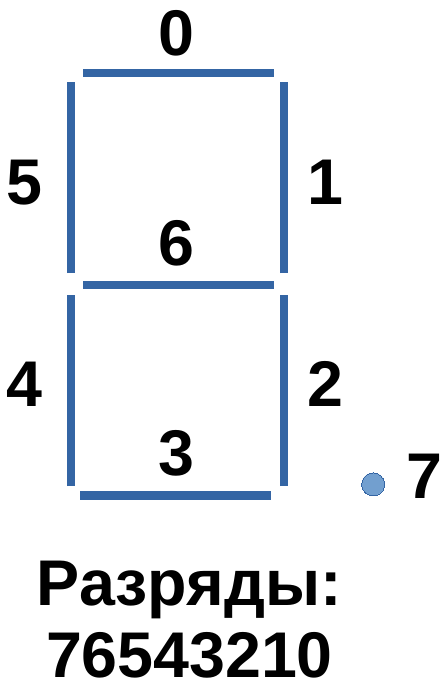
\includegraphics[width=0.3\textwidth]{img/digit-control.png}
    \caption{Отображение сегментов индикатора в данных, передаваемых устройству}
    \label{digit-control}
\end{figure}

\section{Домашнее задание}


% --- Семинар 17. Мультипроцессоры. Специализированные процессоры ---
\chapter[17]{Семинар 17. Таймер. Прерывания по таймеру}

Целью семинара является изучение базовых механизмов синхронизации POSIX Threads, обеспечивающих совместное безконфликтное использование ресурсов. Необходимо провести анализ примеров, демонстрирующих различные методы синхронизации и того, что может получиться при отсутствии синхронизации.

Примерный перечень вопросов:
\begin{enumerate}
    \item Пример 01. Перемножение матриц.  Лучше использовать пример 07 (07. Перемножение матриц. Добавление мьютексов для синхронизации очереди вывода данных), так как там имеется больше информации для вывода данных. Первый вариант связан с тем, что можно после запуска корректной программы закомментировать мьютексы и сопоставить результаты. Возможно, из-за того, что вычислительная нагрузка небольшая и потоки отрабатывают быстро, весь вывод данных и формирование матрицы с результатами на выводе произойдут корректно. Можно запустить программу без мьютексов нескольно раз. Тогда, раскомментировав мьютексы, можно увеличить матрицы, например до 10*10. Создать десяток потоков и повторить еще раз. После этого раскомментировать и посмотреть, произойдет ли изменение вывода. То есть, разобраться с тем, что не всегда очевидно сразу, что синхронизация может понадобиться.
    \item Пример 02 (08. Задача о кольцевом буфере. Использование семафоров для синхронизации потоков). Здесь время не играет определенной роли. Поэтому после демонстрации протокола работающей программы можно посмотреть, что будет если закомментировать по очереди семафоры и мьютексы. Помимо этого можно изменить поведени системы. Например, ускорить писателей и читателей. Или резко увеличить тех или других без изменения временных интервалов. В этих ситуациях интересно посмотреть ожидание, когда буфер будет либо полон, либо пуст.
    \item Пример 03 (09. Задача о кольцевом буфере. Использование условных переменных для синхронизации потоков). Но с другими синхропримитивами. Просто акцентировать на специфике и отличии условных переменных от семафоров. Но так же можно поиграться.
    \item Пример 04 (10. Читатели-писатели с общим одномерным массивом. Использование блокировок).Если успеваем, то можно зацепить этот и следующий. Или перенести на следующий семинар, увязав на нем с OpenMP. Здесь, наверное, можно поиграться только с разными интенсивностями работы читателей и писателей. Тем более, что читатели ничего не меняют. Можно поиграться числом разных потоков или интенсивностью их обращения.
    \item Пример 05 (11. Использование барьеров для синхронизации данных). Пример интересен именно тем, где и как убирать или ставить барьеры. Именно они влияют на синхронизацию двух разделенных массивов. Вариант одного барьера закомментирован. С двумя другими можно тоже поиграться, посмотрев разные варианты. Вплоть до отсутствия барьеров. Мьютексы отвечают за вывод. Поэтому их трогать смысла особого нет. Но тоже можно посмотреть, если будет время.
\end{enumerate}

Во всех альтернативных программах можно использовать код как на Си, так и на плюсах. Они работают одинаково.

Пусть студенты сами сделают прогоны и сформируют результаты.

\section{Домашнее задание}

Перенести задание с предыдущего занятия. Пусть проведут дополнительный анализ на необходимость использования синхронизации.

Что было на предыдущем:

Сделать выслать письменный реферат, в котором оценить возможность параллельного выполнения задания №1 на обработку целочисленных одномерных массивов и использованием методов синхронизации. По своему сделанному варианту. Программу писать не нужно.

% --- Семинар 18. Мультипроцессоры. Специализированные процессоры ---
\chapter[18]{Семинар 18. Программирование ввода--вывода. Использование прерываний}

Целью семинара является продолжение изучения базовых механизмов синхронизации POSIX Threads, обеспечивающих совместное безконфликтное использование ресурсов. Необходимо провести анализ примеров, демонстрирующих различные методы синхронизации и того, что может получиться при отсутствии синхронизации.

Изучение примеров с OpenMP, прилагающихся к лекциям. Предыдущие и эти примеры достаточно короткие. Поэтому можно просто пробежаться. Вполне возможно, что OpenMP придется установить. Обычно пакет openmp. На Убунте не пробовал. Попробую --- сообщу. Все эти примеры я планирую показать на лекции. Но для раздолбаев, которые на лекции не ходят, может оказаться полезным. Заодно все узнают, как установить библиотеку.

После этих примеров обсудить результаты выполнения заданий.

Примерный перечень вопросов (часть перенесена из предыдущего семинара, так как не рассматривалась на лекции):
\begin{enumerate}
    \item Пример 04 (10. Читатели-писатели с общим одномерным массивом. Использование блокировок). Здесь, наверное, можно поиграться только с разными интенсивностями работы читателей и писателей. Тем более, что читатели ничего не меняют. Можно поиграться числом разных потоков или интенсивностью их обращения. В целом основной акцент на самом механизме организации блокировок и поведении участников. В целом ничего хитрого в пояснении и использовании я не вижу.
    \item Пример 05 (11. Использование барьеров для синхронизации данных). Пример интересен именно тем, где и как убирать или ставить барьеры. Именно они влияют на синхронизацию двух разделенных массивов. Вариант одного барьера закомментирован. С двумя другими можно тоже поиграться, посмотрев разные варианты. Вплоть до отсутствия барьеров. Мьютексы отвечают за вывод. Поэтому их трогать смысла особого нет. Но тоже можно посмотреть, если будет время. Ключевая идея связана с независимостью данных и использования барьеров для согласованного изменения своих массивов.
    \item Пример 06 (01. Многопоточный вывод "Hello World"). Данный пример прост. На нем можно увидеть, как работает прагма \verb|#pragma omp parallel|. Можно ее отключить и посмотреть, что получится. Основная идея --- рассмотреть две функции, которые определяют число возможных потоков по ядрам системы и номер текущего потока. Каждый поток обрабатывается независимо и выводит свои данные.
    \item Пример 08 (02. Использование критической секции. Шаг 1). Пример показывает использование критической секции \verb|#pragma omp critical|. В данном случае общая переменная изменяется произвольно, а синхронизация осуществляется по выводу. Как раз можно оценить, что происходит с этой переменной при неправильной установке критической секции.
    \item Пример 09 (03. Использование критической секции. Шаг 2). В этом примере критическая секция установлена на переменной. Но не на выводе данных. Тоже полезно посмотреть рассогласование вывода. Как и в предыдущем случае можно запустить несколько раз, чтобы отследить недетерминированность.
    \item Пример 10 (04. Использование критической секции. Шаг 3). Окончательный пример по критической секции. Имеется выбор конкретного числа потоков. Можно поиграться с этим. Также можно посмотреть потоки с использованием системного монитора. Также там описано использование редукции. Можно поиграться с различными прагмами распараллеливания.
    \item Пример 11 (05. Вычисление интеграла с использованием редукции). Разные варианты и число потоков для просмотра. Тоже можно поиграться с режимами.
\end{enumerate}

Во всех альтернативных программах можно использовать код как на Си, так и на плюсах. Они работают одинаково.

Пусть студенты сами сделают прогоны и сформируют результаты.

\section{Домашнее задание}

Установить на домашней системе openMP и прислать отчет (в виде сканов), демонстрирующих выполнение программы вычисления интеграла с использованием openMP. Использовать свои данные, изменив в программе функцию, используемую для интегрирования и интервалы интегрирования. Три варианта запуска с разными интервалами.

% --- Семинар 19. Мультипроцессоры. Специализированные процессоры ---
\chapter[19]{Семинар 19. Микроархитектура. Предсказание переходов. Кеширование}

Целью семинара является продолжение изучения особенностей организации и использования интерфейса передачи сообщений на основе библиотеки Message Passing Inteface (MPI).

Изучение примеров с MPI, прилагающихся к лекциям. Предыдущие и эти примеры достаточно короткие. Поэтому можно просто пробежаться. Вполне возможно, что MPI придется установить. Пока на Убунте у меня не удалось настроить OpenMPI, хотя сам пакет установился проблемы оказались с настройкой путей к заголовочным файлам. Пока же не проходит компиляция. Не находит этих путей. Конфигурировать пробовал, но пока результа не достигнут. Буду пробовать еще. Не получится --- попробую установить и настроить MPICH. Это еще одна версия MPI, доступная в Убунте. Когда-то она была основной в Linux. Результаты сообщу. Текст подправлю. Также хочу попробовать под Virtual Box Simply Linux.

Есть еще один дежурный вариант, который может устроить всех: установка MPI на рабочей системе. Он есть как под Виндой, так и под Яблоком. Это в принципе можно учесть при раздаче домашнего задания. Если у тебя получится под Линуксом --- попробуй Винду. Можно потом прописать в семинарах. Поищи ссылки в сети. Можешь их вставить в свою презентацию и выложить в семинар. Пусть делают ДЗ на своих ОС. Это непринципиально.

Кстати, отсутствующие а ЛМС семинары я постараюсь обозначить по темам и можно туда включить твои презентации. Лекционные примеры, наверное, переносить не буду, но в последующем что-то можно поискать и добавить. В частности, домашние задания.

\textbf{\textit{Если не получится ничего установить в классе, то можно, как я планирую, посмотреть функционирование кода на проекторе со своего компьютера.}}

Примерный перечень вопросов (часть перенесена из предыдущего семинара, так как не рассматривалась на лекции):
\begin{enumerate}
    \item Пример 01 (01. Простое распределенное приложение: "Привет от MPI"). На нем име можно поиграться как с параметрами файла хостов, так и числом запускаемых процессов. Показать, что при ограниченном числе слотов в конфигурационном файле запуск большего числа процессов не проходит. То же можно просмотреть и без указания слотов в команде, когда раределение процессов по узлам идет по кругу, но до предела, определяемого умолчанием. Расширить этот предел до <<неограниченного>> числа можно использованием опции \verb|--oversubscribe|. Здесь удобно тем, что при превышении числа слотов, указанного в конфигурационном файле, выдается сообщение, подсказывающее о вариантах использования. Еще можно попытаться задать огромное число процессов. Например, 1000. Система должна ругнуться на ограниченность процессов и пайпов, которые она может запустить. Особенно на пайпы, которые, видимо используются внутри MPI.
    \item Пример 02 (02. MPI. Пример передачи и приема сообщений). Пример ориентирован на взаимодействие только двух процессов по простейшему блокирующему передаче и приему. В данном случае интересно обсудить, каким образом осуществляется ограничение процессов. Можно также попробовать предварительно до приема прочитать статус. Посмотрет (count) переданное число байт. Но в целом это базовая схема для различных других вариантов использования. Как варианты, можно предложить сделать модификации, в которых вместо строки осуществляется передача целых, действительных чисел.
    \item Пример 03 (03. MPI. Использование барьеров). Барьерная задача очень проста. Но в принципе на ней можно увидеть, что будет, если барьер убрать. Тогда последнее сообщение, стоящее после барьера, будет выведено не в конце.
    \item Пример 04 (04. MPI. Широковещательная рассылка). Детально разобрать пример, программы, осуществляющей широковещательную рассылку. Можно раскомментировать выводы, демонстрирующие количество процессов коммуникаторах. Позапускать программу с разным числом процессов (начиная с 1). Четным и нечетным. Оценить поведение.
    \item Пример 05 (05. MPI. Вычисление суммы квадратов). Как вариант из предыдущих семинаров: можно увеличить нагрузк на цикл, добавив, например, вычисление квадратного корня или чего-то еще. Также интересно посмотреть вычисление на разном числе узлов с разным и сопоставить время вычислений при одинаковом числе элементов в массиве.
    \item Пример 06 (06. MPI. Вычисление числа Пи). Пример завершает работу при вводе нуля. На нем можно посмотреть широковещательную рассылку, использование суммирования и свертки с применением MPI. Также интересно несколько раз задать разную точность вычисления путем задания количества интервалов. Сопоставить время получения результата.
\end{enumerate}

\section{Домашнее задание}

Установить на домашней системе MPI и прислать отчет (в виде сканов), демонстрирующих выполнение программы осуществляющей пересылки текстовых сообщений между тремя потоками в соответствии со схемой, представленной на слайде 19 лекции по MPI. За основу можно взять пример 02.


% --- Семинар 20. Мультипроцессоры. Специализированные процессоры ---
\chapter[20]{Семинар 20. Микроархитектура. Конвейеризация}

Целью семинара является сопоставление методов псевдопараллельного и параллельного програмирования на примере событийного подхода, используемого в различных системах (C\#, Qt и~др.) и многопоточного программировния на основе \texttt{pthread}. То есть, для упрощения вычислений и привязки к заданию свести тему к многопочности, а не параллелизму в общем виде.

Честно говоря, у меня начинается потеря связи между лекционным материалом и его отображением на практике, что связано с невозможностью воспроизвести на текущем оборудовании ряда задач, которые еще могу рассмотреть на лекции. Поэтому я решил попробовать посвятить семинар материалу, который можно использовать при выполнении четвертого задания, с одной стороны. С другой стороны этот материал можно также использовать для формирования представления о методах программирования, используемых в современных последовательных системах для организации псевдопараллельных вычислений.

Для этого я предлагаю рассмотреть библиотеку Qt и тот подход, который там используется для взаимодействия отдельных функций в асинхронном режиме. На примере программы имитации роста растений и поедающих эту растительность животных рассмотреть поведение системы и попытаться отобразить его (пока концептуально) в поведение многопоточной системы, аналогичной тем программам, которые реализуются в четвертом задании.

Оставшееся время (или, если что-то не пойдет с этим вариантом) можно посвятить разбору третьего задания. Я думаю, что сильно в это погружаться не стоит, так как ключевым является переход к концептуальному обсуждению схемы задачи, описывающей параллелизм и методов ее реализации в реальной многопоточной среде. То есть, рассмотреть на уровне общей структуры, не забираясь в само кодирование. Чтобы при выполнении своих заданий были некоторые стереотипы, куда идти.

Примерный перечень вопросов:
\begin{enumerate}
    \item Краткий рассказ об особенностях событийного программирования на примере практически любых систем. По имеющейся информации нынешние второкурсники изучали основы обработки событий в C\#. Проблемы могут возникнуть с теми, кто пришел с потока ИСП РАН. Можно кратко охарактеризовать на пальцах. Ты ведь знаешь C\# и другие. Можно сориентироваться и на библиотеки Qt. Есть у меня соответствующая лекция для первокурсников. Она будет в 13-м семинаре, как и соответствующие примеры. Обсудить, что программа по сути формируется как набор псевдопараллельных компонент, связанных между собой <<проводами>>, по которым передаются сообщения, являющиеся по сути сигналами. Реализация этого механизма осуществляется за счет формирования очередей сообщений, из которой некоторым диспетчером осуществляется последовательная выборка с запуском очередной функции или метода. При этом ОС система дополнительно управляет переключением потоков, отвечающих за различные другие функции, что в данном случае является несущественным для рассматриваемой программы, но поддерживает общий параллелизм. Псевдопараллелизм поддерживается тем, что сами выполняемые функции не являются нагруженными задачей. \textbf{Но сильно погружаться (заморачиваться) не нужно. На уровне интуиции.} \textit{Можно во время демонстрации примеров.}
    \item Далее (или сразу же) можно привести примеры игры elife, имитирующей поедание растущей травы. Есть (выложена) чужая реализация на JS и моя на Qt. Положил проекты на qmake и cmake. Исходя из этого можно обсудить внутреннюю структуру, например, обработки на JS. Запустить по ходу можно несколько раз. Можно одновременно оба на одном экране.
    \item После этого можно приступить в вариантам возможной реализации с примененим многопоточного программирования. Фиксируя, например, на доске, предлагаемые варианты. Пусть студенты изначально сами предложат версии того, как можно написать параллельную (многопоточную) программу. На первом этапе можно не вдаваться в детали, а породить именно варианты возможного воплощения сценария в потоках. То есть, то что им нужно сделать (сформировать хотя бы один сценарий) по заданию 4. Возможные варианты:
        \begin{itemize}
            \item Один поток --- поведение всей еды, другой --- поведение поедателей. Синхронизация при доступе к поляне.
            \item Каждый поток определяет один элемент еды или поедателя. Поляна --- набор данных вокруг которого идет синхронизация. Здесь речь пойдет о создании потоками новых потоков и завершении тех потоков при соответствующих условиях.
            \item Каждая клетка поляны - поток, который содержит в виде данных одно из состояний (пусто, еда, поедатель). Здесь возникает синхронизации с соседними клетками.
            \item Возможны и другие варианты. Пусть в начале предлагают свои. После этого, если останутся, соответствующие из выше предложенных.
        \end{itemize}
    \item После этого можно обсудить специфику каждого из сценариев. То есть, как и какие порождать потоки. Как их синхронизировать. Где проще организовать. Какой вариант обладает бОльшим параллелизмом. Какие варианты синхронизации возникают. В принципе здесь могут появиться и подварианты. Можно попробовать устроить конкурс: кому какой вариант больше нравится. И разбить анализ по подгруппам. Что у какой получится...
    \item Доводить до реализации не стоит. Но если будет время, то детали каких-то вариантов можно проработать. То есть, именно порождение концептуальных решений.
\end{enumerate}

Остаток занятия или перерыв можно оставить под обсуждение результатов выполнения задания 3

\section{Домашнее задание}

Скорее всего выдавать не стоит, так как дедлайн по заданию 4. Пусть используют идеи в своем варианте.


% --- Семинар 21. Мультипроцессоры. Специализированные процессоры ---
\chapter[21]{Семинар 21. Поддержка многозадачности. Виртуализация. Многоядерность}

Целью семинара является изучение основных принципов подхода, направленного на создание архитектурно-независимых параллельных программ. Основная идея связана с тем, чтобы при разработке программ сделать основной акцент на функциональные и алгоритмические зависимости, максимально абстрагировавшись от использования вычислительных ресурсов.

Для изучения подхода предлагается использовать функционально-потоковую парадигму параллельного программирования. Ее описание, а также язык и IDE представлены на сайте по ссылке: \url{http://softcraft.ru/parallel/fpp/}. В рамках семинара предлагается изучить основные идеи подхода и разобрать особенности построения функционально потоковых параллельных (ФПП) программ. Среда функционирует под Виндой. Программы и сама среда выложены в ЛМС.

Примерный порядок проведения семинара:
\begin{enumerate}
    \item Первоначально предлагается установить и запустить среду. Посмотреть на ее основные элементы управления. Можно практически сразу загрузить файл с множеством функций и на его примере рассмотреть особенности конструкции языка и их использование для описания параллельных вычислений. При этом имеет смысл пользоваться тем описанием, которое лежит на сайте. В целом там вполне понятное описание. Если что по нему непонятно, то могу пояснить.
    \item Далее можно начать понемногу рассматривать основные фунции и оснобенности работы с ними по порядку. На примере функции
    \begin{verbatim}
        ParASMD << funcdef Param
        {
         Param:[+,-,*,/,%]:(.) >>return
        };
    \end{verbatim}
    можно показать, как задается одновременность в обработке одного потока данных. Аргументами функции, задаваемым в табе аргументов может служить любой двухэлементный список. Можно, используя примеры ниже, запускать функцию с любыми тестовыми данными. В приведенных тестовых примерах функции как бы запускаются внутри параллельного списка. То есть, <<одновременно>>. Одновременность была бы при наличии соответствующего параллельного интерпретатора. Можно также пробежаться с пошаговым отладчиком по фунции, чтобы посмотреть как он работает.
    \item На функции вычисления абсолютной величины можно рассмотреть каким образом задаются условия и организуются ветвления.
    \begin{verbatim}
        Abs << funcdef Param
        {
         ({Param:-},{Param}):[(Param,0):(<,=>):?]:.>>return
        };
   \end{verbatim}
   Особенность в том, что нет ветвления потоков, а имеется их выборка из альтернативных вариантов. То есть, поток всегда есть и сводися в общий путь. При этом для того, чтобы ненужные вычисления не выполнялись, используется задержанный список (\verb|{...}|.
   \item При вычислении квадратного корня используется обычный последовательный алгоритм. В принципе здесь можно рассмотреть, как он отображается на информационный граф, когда отстутствует явное управление вычислениями, а используется управленипе по готовности данных. Можно в принципе особо и не рассматривать.
   \item Далее можно остановиться на организации параллельной рекурсии.
   \begin{verbatim}
    VSum << funcdef Param
    {
     Len<<Param:|;
     return<< .^[((Len,2):[<,=,>]):?]^
     ({Param:[]},
     {Param:+},
     {block{
            OddVec<< Param:[(1,Len,2):..];
            EvenVec<< Param:[(2,Len,2):..];
            ([OddVec,EvenVec]:VSum):+ >>break}
     })
    };
   \end{verbatim}
   Пояснить специфику разделения списка данных (вектора) на два посписка, на каждым из которых снова может выполняться дихотомия. В данном случае идет разделение по четным и нечетным элементам. До списка с одним или двумя элементами. Над последним выполняется суммирование, результат поднимается вверх и суммируется с результатом из другого подсписка.
   \item Аналогичный прием можно обобщить на функции высшего порядка.
   \begin{verbatim}
    VHigh << funcdef Param
    {
     Len<<Param:1:|;
     Func<<Param:2;
     return<< .^[((Len,2):[<,=,>]):?]^
     ({Param:1:[]},
     {Param:1:Func},
     {block{
            OddVec<< Param:1:[(1,Len,2):..];
            EvenVec<< Param:1:[(2,Len,2):..];
            ([(OddVec, Func),(EvenVec,Func)]:VHigh):Func >>break}
     })
    };
    \end{verbatim}
    Основная идея здесь заключается в передаче функции в качестве аргумента. Это используется в тестовых примерах.
    \item Далее приведены различные функции работы с векторами. Их можно рассмотреть более бегло, останавливаясь только на конструкциях вызывающих вопросы. Ответы на большую часть вопросов можно получить по ссылке, указанной выше.
    \item И на закуску, если останется время, можно рассмотреть параллельную интерпретацию задачи о Ханойской башне и сортировки, представленные в виде отдельных файлов.
\end{enumerate}

\section{Домашнее задание}

Скорее всего выдавать не стоит, так как дедлайн остается занятие для разбора полетов и то не у всех.

% --- Семинар 22. Мультипроцессоры. Специализированные процессоры ---
\chapter[22]{Семинар 22. }

\chapter{Семинар 22. Мультипроцессоры. Специализированные процессоры}

Целью семинара является изучение основных принципов подхода, направленного на создание архитектурно-независимых параллельных программ. Основная идея связана с тем, чтобы при разработке программ сделать основной акцент на функциональные и алгоритмические зависимости, максимально абстрагировавшись от использования вычислительных ресурсов.

Для изучения подхода предлагается использовать функционально-потоковую парадигму параллельного программирования. Ее описание, а также язык и IDE представлены на сайте по ссылке: \url{http://softcraft.ru/parallel/fpp/}. В рамках семинара предлагается изучить основные идеи подхода и разобрать особенности построения функционально потоковых параллельных (ФПП) программ. Среда функционирует под Виндой. Программы и сама среда выложены в ЛМС.

Примерный порядок проведения семинара:
\begin{enumerate}
    \item Первоначально предлагается установить и запустить среду. Посмотреть на ее основные элементы управления. Можно практически сразу загрузить файл с множеством функций и на его примере рассмотреть особенности конструкции языка и их использование для описания параллельных вычислений. При этом имеет смысл пользоваться тем описанием, которое лежит на сайте. В целом там вполне понятное описание. Если что по нему непонятно, то могу пояснить.
    \item Далее можно начать понемногу рассматривать основные фунции и оснобенности работы с ними по порядку. На примере функции
    \begin{verbatim}
        ParASMD << funcdef Param
        {
         Param:[+,-,*,/,%]:(.) >>return
        };
    \end{verbatim}
    можно показать, как задается одновременность в обработке одного потока данных. Аргументами функции, задаваемым в табе аргументов может служить любой двухэлементный список. Можно, используя примеры ниже, запускать функцию с любыми тестовыми данными. В приведенных тестовых примерах функции как бы запускаются внутри параллельного списка. То есть, <<одновременно>>. Одновременность была бы при наличии соответствующего параллельного интерпретатора. Можно также пробежаться с пошаговым отладчиком по фунции, чтобы посмотреть как он работает.
    \item На функции вычисления абсолютной величины можно рассмотреть каким образом задаются условия и организуются ветвления.
    \begin{verbatim}
        Abs << funcdef Param
        {
         ({Param:-},{Param}):[(Param,0):(<,=>):?]:.>>return
        };
   \end{verbatim}
   Особенность в том, что нет ветвления потоков, а имеется их выборка из альтернативных вариантов. То есть, поток всегда есть и сводися в общий путь. При этом для того, чтобы ненужные вычисления не выполнялись, используется задержанный список (\verb|{...}|.
   \item При вычислении квадратного корня используется обычный последовательный алгоритм. В принципе здесь можно рассмотреть, как он отображается на информационный граф, когда отстутствует явное управление вычислениями, а используется управленипе по готовности данных. Можно в принципе особо и не рассматривать.
   \item Далее можно остановиться на организации параллельной рекурсии.
   \begin{verbatim}
    VSum << funcdef Param
    {
     Len<<Param:|;
     return<< .^[((Len,2):[<,=,>]):?]^
     ({Param:[]},
     {Param:+},
     {block{
            OddVec<< Param:[(1,Len,2):..];
            EvenVec<< Param:[(2,Len,2):..];
            ([OddVec,EvenVec]:VSum):+ >>break}
     })
    };
   \end{verbatim}
   Пояснить специфику разделения списка данных (вектора) на два посписка, на каждым из которых снова может выполняться дихотомия. В данном случае идет разделение по четным и нечетным элементам. До списка с одним или двумя элементами. Над последним выполняется суммирование, результат поднимается вверх и суммируется с результатом из другого подсписка.
   \item Аналогичный прием можно обобщить на функции высшего порядка.
   \begin{verbatim}
    VHigh << funcdef Param
    {
     Len<<Param:1:|;
     Func<<Param:2;
     return<< .^[((Len,2):[<,=,>]):?]^
     ({Param:1:[]},
     {Param:1:Func},
     {block{
            OddVec<< Param:1:[(1,Len,2):..];
            EvenVec<< Param:1:[(2,Len,2):..];
            ([(OddVec, Func),(EvenVec,Func)]:VHigh):Func >>break}
     })
    };
    \end{verbatim}
    Основная идея здесь заключается в передаче функции в качестве аргумента. Это используется в тестовых примерах.
    \item Далее приведены различные функции работы с векторами. Их можно рассмотреть более бегло, останавливаясь только на конструкциях вызывающих вопросы. Ответы на большую часть вопросов можно получить по ссылке, указанной выше.
    \item И на закуску, если останется время, можно рассмотреть параллельную интерпретацию задачи о Ханойской башне и сортировки, представленные в виде отдельных файлов.
\end{enumerate}

\section{Домашнее задание}

Скорее всего выдавать не стоит, так как дедлайн остается занятие для разбора полетов и то не у всех.


% --- Заключение -------------------------------------------
\chapter*{Заключение}
\addcontentsline{toc}{chapter}{Заключение}

%\centering
\framebox[0.8\textwidth][l]{\textit{Продолжение следует...}}


% --- Приложение А. Задание 1. Вычисления с плавающей точкой ---
\chapter*{Приложение А Задание 1. Целочисленная арифметика и массивы}
\addcontentsline{toc}{chapter}{Приложение А Задание 1. Целочисленная арифметика и массивы}

Разработать программу, которая получает одномерный массив \textbf{A$_N$}, после чего формирует из элементов массива \textbf{A} новый массив \textbf{B} по правилам, указанным в варианте, и выводит его. Память под массивы может выделяться статически, на стеке, в области кучи по выбору разработчика. При решении задачи необходимо использовать подпрограммы для реализации ввода, вывода и формирования нового массива. Ввод-вывод элементов реализовать в окно выполнения эмулятора с использованием его системных вызовов.

\begin{enumerate}
    \item Сформировать массив \textbf{B} из положительных элементов массива \textbf{А}.
    \item Сформировать массив \textbf{B} только из тех элементов массива \textbf{А}, которые не совпадают с его первым и последним элементами.
    \item  Сформировать массив \textbf{B} из сумм соседних элементов \textbf{A} по следующим правилам:
           \textbf{ B$_0$ = A$_0$ + A$_1$, B$_1$ = A$_1$ + A$_2$, ... }
    \item Массив \textbf{B} формируется по следующим правилам:
    \begin{itemize}
        \item \textbf{B$_i$ = 1, если A$_i$ > 0},
        \item \textbf{B$_i$ = -1, если A$_i$ < 0},
        \item \textbf{B$_i$ = 0, если A$_i$ = 0}.
    \end{itemize}
    \item Сформировать массив \textbf{B}, состоящий из элементов массива \textbf{А}, значение которых не совпадает с дополнительно введённым числом \textbf{X}.
    \item Сформировать массив \textbf{B}, состоящи из элементов массива \textbf{A}, значения которых кратны введенному числу \textbf{X}.
    \item Сформировать массив \textbf{B} из индексов положительных элементов массива \textbf{A}.
    \item Сформировать массив \textbf{B} по следующим правилам:
    \begin{itemize}
        \item \textbf{если A$_i$ > 5, то увеличить элемент B$_i$ на 5,},
        \item \textbf{eсли A$_i$ < -5, то уменьшить B$_i$ на 5,},
        \item \textbf{остальные B$_i$ обнулить.}.
    \end{itemize}
    \item Сформировать массив \textbf{B} из нечётных элементов массива \textbf{A}.
    \item Сформировать массив \textbf{B} из отрицательных элементов массива \textbf{A}, расположенных обратном порядке.
    \item Сформировать массив \textbf{B} из элементов \textbf{A}, расположенных в обратном порядке, исключая первый положительный элемент.
    \item Сформировать массив \textbf{B} из элементов массива \textbf{A}, исключив первый
    положительный и последний отрицательный элементы.
    \item Сформировать массив \textbf{B} из элементов массива \textbf{A}, за исключением элементов, значения которых совпадают с минимальным элементом массива \textbf{A}.
    \item Сформировать массив \textbf{B} из элементов массива \textbf{A} заменой всех отрицательных значений на максимум из массива \textbf{A}.
    \item Сформировать массив \textbf{B} из элементов массива \textbf{A} заменой всех нулевых элементов значением минимального элемента.
    \item Сформировать массив \textbf{B} из элементов массива \textbf{A}, заменой на среднее арифметическое тех значений, которые больше среднего арифметического.
    \item Сформировать массив \textbf{B} из элементов массива \textbf{A}, расположенных после последнего положительного элемента.
    \item  Сформировать массив \textbf{B} из элементов массива \textbf{A} уменьшением всех элементов, расположенных до первого положительного, на \textbf{5}.
    \item Сформировать массив \textbf{B} из элементов массива \textbf{A} заменой нулевых элементов, предшествующих первому отрицательному, единицей.
    \item  Сформировать массив \textbf{B} из элементов массива \textbf{A} перестановкой местами минимального и первого элементов.
    \item Сформировать отсортированный по возрастанию массив \textbf{B} из элементов массива \textbf{A}.
    \item  Сформировать отсортированный по убыванию массив \textbf{B} из элементов массива~\textbf{A}.
    \item Сформировать массив \textbf{B}, элементы которого являются расстояниями пройденными телом при свободном падении на землю за время в секундах, указанное в массиве \textbf{A}. Решение получить в целых числах, приняв ускорение свободного падения за \textbf{10}.
    \item Сформировать массив \textbf{B} из элементов массива \textbf{A} поменяв местами элементы, стоящие на чётных и нечётных местах:
            \textbf{A$_0$ $\leftrightarrow$ A$_1$; A$_2$ $\leftrightarrow$ A$_3$ ...}
    \item Сформировать массив \textbf{B} из элементов массива \textbf{A} заменив все положительные числа значением \textbf{2}, а отрицательные — увеличить на \textbf{5}.
    \item Сформировать массив \textbf{B} из сумм трех соседних элементов массива \textbf{A}, сумма значений которых максимальна. Если элементов в массиве \textbf{А} менее трёх, то заполнить массив \textbf{В} нулями.
    \item Сформировать массив \textbf{B} из элементов массива \textbf{A}. Элементы массива \textbf{А}, оканчивающиеся цифрой \textbf{4}, уменьшить вдвое.
    \item Сформировать массив \textbf{B} из элементов массива \textbf{A}, которые образуют неубывающую последовательность. Неубывающей последовательностью считать элементы идущие подряд, которые равны между собой или каждый последующий больше предыдущего.
    \item Сформировать массив \textbf{B} из произведения соседних элементов \textbf{A} по следующему правилу: \textbf{B$_0$ = A$_0$ * A$_m$ , B$_1$ = A$_1$ * A$_m$, ...}, где \textbf{m} – либо номер первого четного отрицательного элемента массива А, либо номер последнего элемента, если в массиве А нет отрицательных элементов.
    \item Сформировать массив \textbf{B} из тех элементов массива \textbf{A}, которые больше, чем элементы, стоящие перед ними.
    \item Сформировать массив \textbf{B} из элементов массива \textbf{A} в следующем порядке: сначала заполняем массив \textbf{В} числами, стоящими на нечетных местах, а затем - стоящие на четных местах в массиве \textbf{А}.
    \item Сформировать массив \textbf{B} из элементов массива \textbf{A}, которые меньше суммы элементов, расположенных на четных местах.
    \item Сформировать массив \textbf{B} на основе элементов массива \textbf{A}, полученных как разность соседних элементов.
    \item Сформировать массив \textbf{B} из элементов массива \textbf{A} заменив элементы на четным местах суммой всех положительных элементов, а элементы на нечетных местах суммой отрицательных элементов.
    \item Сформировать массив \textbf{B} из элементов массива \textbf{A} сгруппировав положительные элементы массива \textbf{А} в начале массива \textbf{В}, а отрицательные --- в конце.
    \item Сформировать массив \textbf{B} из элементов массива \textbf{A} сгруппировав элементы с четными индексами в начале массива \textbf{В} , а элементы с нечетными индексами сгруппировать в конце массива \textbf{В}.
    \item Сформировать массив \textbf{B} из элементов массива \textbf{A} в следующем порядке: элементы с индексами \textbf{i $\le$ (N + 1)/2} переместить на позиции с четными индексами массива \textbf{В} с сохранением их исходного порядка относительно друг друга, а оставшиеся элементы (\textbf{i $>$ (N + 1)/2}) разместить на позициях с нечетными индексами массива \textbf{В} также с сохранением их исходного порядка.
    \item Сформировать массив \textbf{B} из элементов массива \textbf{A}, которые одновременно имеют четные и отрицательные значения.
    \item Сформировать массив \textbf{B}, элементы которого являются площадью прямоугольников со сторонами указанные в массиве \textbf{A}: \textbf{B$_i$ = A$_i$ * A$_{i+1}$}.
    \item Сформировать массив \textbf{B} из суммы соседних элементов \textbf{A} по следующему правилу: \textbf{B$_0$ = A$_0$, B$_1$ = A$_0$ + A$_1$, ..., B$_m$ = A$_0$ + ... + A$_m$}, где \textbf{m} – номер
    первого элемента массива \textbf{А} большего, чем среднее арифметического этого массива.
\end{enumerate}

% --- Приложение Б. Задание 2. Вычисления с плавающей точкой ---
\chapter*{Приложение Б Задание 2. Вычисления с плавающей точкой}
\addcontentsline{toc}{chapter}{Приложение Б Задание 2. Вычисления с плавающей точкой}

Разработать программы на языках программирования C и Ассемблер, выполняющие вычисления над числами с плавающей точкой. Разработанные программы должны принимать числа в допустимом диапазоне. Например, нужно учитывать области определения и допустимых значений, если это связано с условием задачи.

\begin{enumerate}
    \item Разработать программу, вычисляющую с помощью степенного ряда с точностью не хуже 0,05\% значение функции $\sqrt{1+x}$ для  заданного параметра \textit{x}.
    \item Разработать программу, вычисляющую с помощью степенного ряда с точностью не хуже 0,1\%  значение функции гиперболического синуса $\sh{(x)} = (e^x-e^{-x})/2$ для  заданного параметра \textit{x}.
    \item Разработать программу, вычисляющую с помощью степенного ряда с точностью не хуже 0,1\% значение функции $\cos{(x)}$ для  заданного параметра \textit{x}.
    \item Разработать программу, вычисляющую с помощью степенного ряда с точностью не хуже 0,1\% значение биномиальной функции $(1+x)^{m}$ для конкретных параметров \textit{m} и \textit{x}.
    \item Разработать программу, вычисляющую с помощью степенного ряда с точностью не хуже 0,05\%  значение функции $\arcsin{(x)}$ для  заданного параметра \textit{x}.
    \item Разработать программу, вычисляющую с помощью степенного ряда с точностью не хуже 0,05\%  значение функции $1/e^x$ для  заданного параметра \textit{x}.
    \item Разработать программу, вычисляющую с помощью степенного ряда с точностью не хуже 0,05\% значение функции $\sin{(x)}$ для  заданного параметра \textit{x}.
    \item Разработать программу, вычисляющую с помощью степенного ряда с точностью не хуже 0,1\% значение функции $\arccos(x)$ для  заданного параметра \textit{x}.
    \item Разработать программу, вычисляющую с помощью степенного ряда с точностью не хуже 0,05\% значение функции $\arctan{(x)}$ для  заданного параметра \textit{x}.
	\item Разработать программу, вычисляющую с помощью степенного ряда с точностью не хуже 0,05\% значение функции гиперболического тангенса $\tanh(x)=(e^x-e^{-x})/(e^x+e^{-x})$ для  заданного параметра~\textit{x}.
	\item Разработать программу, вычисляющую с помощью степенного ряда с точностью не хуже 0,05\% значение функции $\textit{1/(1-x)}$ для  заданного параметра \textit{x}.
	\item Разработать программу, вычисляющую с помощью степенного ряда с точностью не хуже 0,05\% значение функции $\tan(x)$ для  заданного параметра \textit{x}.
	\item Разработать программу, вычисляющую с помощью степенного ряда с точностью не хуже 0,1\%  значение функции $e^x$ для  заданного параметра \textit{x}.
    \item Разработать программу, вычисляющую с помощью степенного ряда с точностью не хуже 0,1\% значение функции гиперболического котангенса $\cth{(x)}=(e^x+e^{-x})/(e^x-e^{-x})$ для  заданного параметра~\textit{x}.
    \item Разработать программу, вычисляющую с помощью степенного ряда с точностью не хуже 0,05\% значение функции гиперболического косинуса $\ch(x)=(e^x+e^{-x})/2$ для  заданного параметра x.
    \item Разработать программу, вычисляющую с помощью степенного ряда с точностью не хуже 0,05\% значение функции $e^{-x}$ для  заданного параметра \textit{x}.
	\item Разработать программу, вычисляющую с помощью степенного ряда с точностью не хуже 0,1\% значение функции $\ln{(1-x)}$ для  входного параметра \textit{x}.
    \item Разработать программу вычисления корня квадратного по итерационной формуле Герона Александрийского с точностью не хуже 0,05\%.
	\item Разработать программу вычисления корня кубического из заданного числа согласно быстро сходящемуся итерационному алгоритму определения корня \textit{n}-ной степени с точностью не хуже 0,05\%.
    \item Разработать программу вычисления числа $\pi$ с точностью не хуже 0,05\% посредством произведения элементов ряда Виета.
    \item Разработать программу вычисления числа $\pi$ с точностью не хуже 0,05\% посредством ряда Нилаканта.
    \item Разработать программу вычисления числа $\pi$ с точностью не хуже 0,1\% посредством дзета-функции Римана.
    \item Разработать программу вычисления числа $\pi$ с точностью не хуже 0,05\% посредством произведения элементов ряда Валлиса.
    \item Разработать программу, вычисляющую с помощью  ряда Эйлера с точностью не хуже 0,1\% значение числа \textit{e}.
    \item Разработать программу, решающую вопрос о принадлежности заданных 4-х точек одной окружности.
    \item Разработать программу вычисления корня пятой степени согласно быстро сходящемуся итерационному алгоритму определения корня \textit{n}-той степени с точностью не хуже 0,1\%.
    \item Разработать программу интегрирования функции $y=a+b*x^{-2}$ (задаётся двумя числами а,b) в заданном диапазоне (задаётся так же) методом Симпсона (точность вычислений = 0.0001).
    \item Разработать программу численного интегрирования функции $y=a+b*x^4$ (задаётся действительными числами а,b) в определённом диапазоне целых (задаётся так же) методом прямоугольников с избытком (точность вычислений = 0.0001).
    \item Разработать программу численного интегрирования функции $y=a+b*x^{-4}$ (задаётся действительными числами а,b) в определённом диапазоне целых (задаётся так же) методом средних (точность вычислений = 0.0001).
    \item Разработать программу численного интегрирования функции $y=a+b*x^3$ (задаётся действительными числами а,b) в определённом диапазоне целых (задаётся так же) методом трапеций (точность вычислений = 0.0001).
    \item Разработать программу численного интегрирования функции $y=a+b*x^3$ (задаётся действительными числами а,b) в определённом диапазоне целых (задаётся так же) методом прямоугольников с недостатком (точность вычислений = 0.0001).
    \item Разработать программу, определяющую корень уравнения $2^{x^{2}+1}+x^2-4=0$ методом половинного деления с точностью от 0,001 до 0,00000001 в диапазоне [0;1]. Если диапазон некорректен, то подобрать корректный диапазон.
    \item Разработать программу, определяющую корень уравнения $x^3-0.5x^2+0.2x-4=0$ методом половинного деления с точностью  от 0,001 до 0,00000001 в диапазоне [1;3]. Если диапазон некорректен, то подобрать корректный диапазон.
    \item Разработать программу, определяющую корень уравнения $x^4+2x^3-x-1=0$ методом половинного деления с точностью = от 0,001 до 0,00000001 в диапазоне [0;1]. Если диапазон некорректен, то подобрать корректный диапазон.
    \item Разработать программу, определяющую корень уравнения $x^4-x^3-2.5=0$ методом хорд с точностью от 0,001 до 0,00000001 в диапазоне [1;2]. Если диапазон некорректен, то подобрать корректный диапазон.
    \item Разработать программу, определяющую корень уравнения $2^{x^{2}+1}+x-3=0$ методом хорд с точностью от 0,001 до 0,00000001 в диапазоне [2;3]. Если диапазон некорректен, то подобрать корректный диапазон.
    \item Разработать программу, определяющую корень уравнения $x^5-x-0.2=0$ методом хорд с точностью от 0,001 до 0,00000001 в диапазоне [1;1.1]. Если диапазон некорректен, то подобрать корректный диапазон.
\end{enumerate}

% --- Приложение В. Задание 3. Обработка строк символов ---
\chapter*{Приложение В Задание 3. Обработка строк символов}
\addcontentsline{toc}{chapter}{Приложение В Задание 3. Обработка строк символов}

\textit{ASCII-строка --- строка, содержащая символы таблицы кодировки ASCII.} (\url{https://ru.wikipedia.org/wiki/ASCII}). Размер строки может быть достаточно большим, чтобы вмещать многостраничные тексты, например, главы из книг, если задача связана с использованием файлов или строк, порождаемых генератором случайных чисел. Тексты при этом могут не нести смыслового содержания. Для обработки в программе предлагается использовать данные, содержащие символы только из первой половины таблицы (коды в диапазоне 0--127$_{10}$), что связано с использованием кодировки UTF-8 в ОС Linux в качестве основной. Символы, содержащие коды выше 127$_{10}$, должны отсутствовать во входных данных кроме оговоренных специально случаев.

\begin{enumerate}
    \item Разработать программу, которая <<переворачивает>> заданную позициями \textbf{N$_1$--N$_2$} часть ASCII--строки символов (\textbf{N$_1$, N$_2$} вводятся как параметры).
    \item Разработать программу, находящую в заданной ASCII--строке первую  при обходе \textbf{от конца к началу} последовательность \textbf{N} символов, каждый элемент которой определяется по условию <<больше предшествующего>> (\textbf{N} вводится в качестве параметра).
    \item Разработать программу, находящую в заданной ASCII-строке первую слева направо последовательность \textbf{N} символов, каждый элемент которой определяется по условию <<меньше предшествующего>> (\textit{\textbf{N} вводится как отдельный параметр}).
    \item Разработать программу, находящую в заданной ASCII-строке последнюю при перемещении слева направо последовательность \textbf{N} символов, каждый элемент которой определяется по условию <<больше предшествующего>> (\textit{\textbf{N} вводится как отдельный параметр}).
    \item Разработать программу, заменяющую все строчные гласные буквы в заданной ASCII-строке заглавными.
    \item Разработать программу, заменяющую все согласные буквы в заданной ASCII-строке их \textbf{ASCII кодами в десятичной системе счисления}.
    \item Разработать программу, заменяющую все гласные буквы в заданной ASCII-строке их \textbf{ASCII кодами в шестнадцатиричной системе счисления}. Код каждого символа задавать в формате <<\textbf{0xDD}>>, где \textbf{D} --- шестнадцатиричная цифра от 0 до F.
    \item Разработать программу, заменяющую все цифры (за исключением нуля) в заданной ASCII-строке \textbf{римскими цифрами}. То есть, соответствующим комбинациями букв для цифр от 1 до 9.
    \item Разработать программу, которая <<\textbf{переворачивает на месте}>> заданную ASCII-строку символов (не копируя строку в другой буфер).
    \item Разработать программу, которая меняет на обратный порядок следования символов \textbf{каждого слова} в ASCII-строке символов. Порядок слов остается неизменным. Слова состоят только из букв. Разделителями слов являются все прочие символы.
    \item Разработать программу вычисления \textbf{отдельно количества гласных и согласных букв} в ASCII-строке.
    \item Разработать программу, определяющую \textbf{минимальный и максимальный (по числовому значению) символ в заданной} ASCII-строке.
    \item Разработать программу, заменяющую все строчные буквы в заданной ASCII-строке прописными, а прописные буквы --- строчными.
    \item Разработать программу, вычисляющую отдельно \textbf{число прописных и строчных букв} в заданной ASCII-строке.
    \item Разработать программу, которая на основе заданной ASCII-строки символов, решает вопрос, является ли данная строка \textbf{палиндромом}.
    \item Разработать программу, которая вычисляет \textbf{количество цифр и букв} в заданной ASCII-строке.
    \item Разработать программу, которая \textbf{меняет на обратный порядок следование слов} в ASCII-строке символов.
    \item Разработать программу, \textbf{заменяющую все согласные буквы в заданной ASCII-строке на заглавные}.
    \item Разработать программу, вычисляющую число вхождений различных \textbf{отображаемых символов} в заданной ASCII-строке.
    \item Разработать программу, вычисляющую \textbf{число вхождений различных цифр} в заданной ASCII-строке.
    \item Разработать программу, осуществляющую \textbf{нахождение суммы всех цифр} в заданной ASCII-строке.
    \item Разработать программу, вычисляющую \textbf{число вхождений различных знаков препинания} в заданной ASCII-строке.
    \item Разработать программу, которая ищет в ASCII-строке заданную подстроку и возвращает \textbf{индекс первого символа первого вхождения подстроки в строке}. Подстрока вводится как параметр.
    \item Разработать программу, которая ищет в ASCII-строке заданную подстроку и возвращает \textbf{список индексов первого символа для всех вхождений} подстроки в строке. Подстрока вводится как параметр.
    \item Разработать программу, которая определяет в ASCII-строке \textbf{частоту встречаемости различных идентификаторов}, являющихся словами, состоящими из букв и цифр, начинающихся с буквы. Разделителями являются все другие символы. Для тестирования можно использовать программы, написанные на различных языках программирования.
    \item Разработать программу, которая определяет \textbf{количество целых чисел} в ASCII-строке. числа состоят из цифр от 0 до 9. Разделителями являются все другие символы.
    \item Разработать программу, которая определяет \textbf{частоту встречаемости (сколько раз встретилось в тексте) пяти ключевых слов языка программирования C}, в произвольной  ASCII-строке. Ключевые слова не должны являться частью идентификаторов. Пять искомых ключевых слов выбрать \textbf{по своему усмотрению}. Тестировать можно на файлах программ.
    \item Разработать программу, которая в заданной ASCII-строке определяет \textbf{корректность вложенности круглых скобок} <<\verb|(|>> и <<\verb|)|>>. Необходимо учесть, что вложенные скобки могут образовывать в тексте различные группы. Например: \verb|...(...)...(...)...|.
    \item Разработать программу, которая ищет в ASCII-строке \textbf{слова --- палиндромы и формирует из них новую строку}, в которой слова разделяются пробелами. Слова состоят из букв. Все остальные символы являются разделителями слов.
    \item Разработать программу, которая ищет в ASCII-строке слова, \textbf{начинающиеся с заглавной буквы и формирует из них новую строку}, в которой слова разделяются пробелами. Слова состоят из букв. Все остальные символы являются разделителями слов.
    \item Разработать программу, которая ищет в ASCII-строке \textbf{целые числа и формирует из них новую строку}, в которой числа разделяются знаком <<\verb|+|>>. Слова состоят из букв. Все остальные символы являются разделителями слов.
    \item Разработать программу, которая на основе анализа двух входных ASCII-строк формирует на выходе две другие строки. В первой из выводимых строк содержатся символы, которых нет во второй исходной строке. Во второй выводимой строке содержатся символы, отсутствующие в первой входной строке (\textbf{разности символов}). Каждый символ в соответствующей выходной строке должен встречаться только один раз.
    \item Разработать программу, которая на основе анализа двух ASCII-строк формирует на выходе строку, содержащую символы, присутствующие в обеих строках (\textbf{пересечение символов}). Каждый символ в соответствующей выходной строке должен встречаться только один раз.
    \item Разработать программу, которая на основе анализа двух ASCII-строк формирует на выходе строку, содержащую символы, присутствующие в одной или другой (\textbf{объединение символов}). Каждый символ в соответствующей выходной строке должен встречаться только один раз
\end{enumerate}

% --- Приложение Г. Задание 4. Взаимодействие с устройствами ввода-вывода ---
\chapter*{Приложение Г Задание 4. Обработка строк символов}
\addcontentsline{toc}{chapter}{Приложение Г Задание 4. Обработка строк символов}

\textit{ASCII-строка --- строка, содержащая символы таблицы кодировки ASCII.} (\url{https://ru.wikipedia.org/wiki/ASCII}). Размер строки может быть достаточно большим, чтобы вмещать многостраничные тексты, например, главы из книг, если задача связана с использованием файлов или строк, порождаемых генератором случайных чисел. Тексты при этом могут не нести смыслового содержания. Для обработки в программе предлагается использовать данные, содержащие символы только из первой половины таблицы (коды в диапазоне 0--127$_{10}$), что связано с использованием кодировки UTF-8 в ОС Linux в качестве основной. Символы, содержащие коды выше 127$_{10}$, должны отсутствовать во входных данных кроме оговоренных специально случаев.

\begin{enumerate}
    \item Разработать программу, которая <<переворачивает>> заданную позициями \textbf{N$_1$--N$_2$} часть ASCII--строки символов (\textbf{N$_1$, N$_2$} вводятся как параметры).
    \item Разработать программу, находящую в заданной ASCII--строке первую  при обходе \textbf{от конца к началу} последовательность \textbf{N} символов, каждый элемент которой определяется по условию <<больше предшествующего>> (\textbf{N} вводится в качестве параметра).
    \item Разработать программу, находящую в заданной ASCII-строке первую слева направо последовательность \textbf{N} символов, каждый элемент которой определяется по условию <<меньше предшествующего>> (\textit{\textbf{N} вводится как отдельный параметр}).
    \item Разработать программу, находящую в заданной ASCII-строке последнюю при перемещении слева направо последовательность \textbf{N} символов, каждый элемент которой определяется по условию <<больше предшествующего>> (\textit{\textbf{N} вводится как отдельный параметр}).
    \item Разработать программу, заменяющую все строчные гласные буквы в заданной ASCII-строке заглавными.
    \item Разработать программу, заменяющую все согласные буквы в заданной ASCII-строке их \textbf{ASCII кодами в десятичной системе счисления}.
    \item Разработать программу, заменяющую все гласные буквы в заданной ASCII-строке их \textbf{ASCII кодами в шестнадцатиричной системе счисления}. Код каждого символа задавать в формате <<\textbf{0xDD}>>, где \textbf{D} --- шестнадцатиричная цифра от 0 до F.
    \item Разработать программу, заменяющую все цифры (за исключением нуля) в заданной ASCII-строке \textbf{римскими цифрами}. То есть, соответствующим комбинациями букв для цифр от 1 до 9.
    \item Разработать программу, которая <<\textbf{переворачивает на месте}>> заданную ASCII-строку символов (не копируя строку в другой буфер).
    \item Разработать программу, которая меняет на обратный порядок следования символов \textbf{каждого слова} в ASCII-строке символов. Порядок слов остается неизменным. Слова состоят только из букв. Разделителями слов являются все прочие символы.
    \item Разработать программу вычисления \textbf{отдельно количества гласных и согласных букв} в ASCII-строке.
    \item Разработать программу, определяющую \textbf{минимальный и максимальный (по числовому значению) символ в заданной} ASCII-строке.
    \item Разработать программу, заменяющую все строчные буквы в заданной ASCII-строке прописными, а прописные буквы --- строчными.
    \item Разработать программу, вычисляющую отдельно \textbf{число прописных и строчных букв} в заданной ASCII-строке.
    \item Разработать программу, которая на основе заданной ASCII-строки символов, решает вопрос, является ли данная строка \textbf{палиндромом}.
    \item Разработать программу, которая вычисляет \textbf{количество цифр и букв} в заданной ASCII-строке.
    \item Разработать программу, которая \textbf{меняет на обратный порядок следование слов} в ASCII-строке символов.
    \item Разработать программу, \textbf{заменяющую все согласные буквы в заданной ASCII-строке на заглавные}.
    \item Разработать программу, вычисляющую число вхождений различных \textbf{отображаемых символов} в заданной ASCII-строке.
    \item Разработать программу, вычисляющую \textbf{число вхождений различных цифр} в заданной ASCII-строке.
    \item Разработать программу, осуществляющую \textbf{нахождение суммы всех цифр} в заданной ASCII-строке.
    \item Разработать программу, вычисляющую \textbf{число вхождений различных знаков препинания} в заданной ASCII-строке.
    \item Разработать программу, которая ищет в ASCII-строке заданную подстроку и возвращает \textbf{индекс первого символа первого вхождения подстроки в строке}. Подстрока вводится как параметр.
    \item Разработать программу, которая ищет в ASCII-строке заданную подстроку и возвращает \textbf{список индексов первого символа для всех вхождений} подстроки в строке. Подстрока вводится как параметр.
    \item Разработать программу, которая определяет в ASCII-строке \textbf{частоту встречаемости различных идентификаторов}, являющихся словами, состоящими из букв и цифр, начинающихся с буквы. Разделителями являются все другие символы. Для тестирования можно использовать программы, написанные на различных языках программирования.
    \item Разработать программу, которая определяет \textbf{количество целых чисел} в ASCII-строке. числа состоят из цифр от 0 до 9. Разделителями являются все другие символы.
    \item Разработать программу, которая определяет \textbf{частоту встречаемости (сколько раз встретилось в тексте) пяти ключевых слов языка программирования C}, в произвольной  ASCII-строке. Ключевые слова не должны являться частью идентификаторов. Пять искомых ключевых слов выбрать \textbf{по своему усмотрению}. Тестировать можно на файлах программ.
    \item Разработать программу, которая в заданной ASCII-строке определяет \textbf{корректность вложенности круглых скобок} <<\verb|(|>> и <<\verb|)|>>. Необходимо учесть, что вложенные скобки могут образовывать в тексте различные группы. Например: \verb|...(...)...(...)...|.
    \item Разработать программу, которая ищет в ASCII-строке \textbf{слова --- палиндромы и формирует из них новую строку}, в которой слова разделяются пробелами. Слова состоят из букв. Все остальные символы являются разделителями слов.
    \item Разработать программу, которая ищет в ASCII-строке слова, \textbf{начинающиеся с заглавной буквы и формирует из них новую строку}, в которой слова разделяются пробелами. Слова состоят из букв. Все остальные символы являются разделителями слов.
    \item Разработать программу, которая ищет в ASCII-строке \textbf{целые числа и формирует из них новую строку}, в которой числа разделяются знаком <<\verb|+|>>. Слова состоят из букв. Все остальные символы являются разделителями слов.
    \item Разработать программу, которая на основе анализа двух входных ASCII-строк формирует на выходе две другие строки. В первой из выводимых строк содержатся символы, которых нет во второй исходной строке. Во второй выводимой строке содержатся символы, отсутствующие в первой входной строке (\textbf{разности символов}). Каждый символ в соответствующей выходной строке должен встречаться только один раз.
    \item Разработать программу, которая на основе анализа двух ASCII-строк формирует на выходе строку, содержащую символы, присутствующие в обеих строках (\textbf{пересечение символов}). Каждый символ в соответствующей выходной строке должен встречаться только один раз.
    \item Разработать программу, которая на основе анализа двух ASCII-строк формирует на выходе строку, содержащую символы, присутствующие в одной или другой (\textbf{объединение символов}). Каждый символ в соответствующей выходной строке должен встречаться только один раз
\end{enumerate}



% --- Библиография -------------------------------------------
\begin{thebibliography}{00}
%\addcontentsline{toc}{section}{Литература}

\bibitem
{risc-v}
RISC-V International. Описание архитектуры и ее обоснование.
--- \url{https://riscv.org/}

\bibitem
{Harris}
Сара Л. Харрис, Дэвид Харрис.
Цифровая схемотехника и архитектура компьютера: RISC-V / пер. с англ. В. С. Яценкова, А. Ю. Романова; под ред. А. Ю. Романова. --- М.: ДМК Пресс, 2021. --- 810 с.

\bibitem
{Borin}
Edson Borin
An Introduction to Assembly Programming with RISC-V /
Document version: May 9, 2022
--- \url{https://riscv-programming.org/}


\bibitem
{kur-2022}
Курячий Георгий. Архитектура и язык ассемблера RISC-V. Весна 2022.
--- \url{http://uneex.ru/LecturesCMC/ArchitectureAssembler2022}

\bibitem
{aps-git}
Семестровый забег "Архитектур процессорных систем"
--- \url{https://github.com/MPSU/APS}

\bibitem
{kur-youtube-2022}
[UNИX] Архитектура и язык ассемблера RISC-V. Видео лекции. Весна 2022.
--- \url{https://www.youtube.com/playlist?list=PL6kSdcHYB3x6cjkby4H1RuRMzfbEGSNBi}

\bibitem
{aps-youtube}
Архитектуры процессорных систем
--- \url{https://www.youtube.com/c/%D0%90%D0%9F%D0%A1%D0%9F%D0%BE%D0%BF%D0%BE%D0%B2}

\bibitem
{RARS}
RARS -- RISC-V Assembler and Runtime Simulator
--- \url{https://github.com/TheThirdOne/rars}

\bibitem
{Ripes}
Ripes. A visual computer architecture simulator and assembly code editor.
--- \url{https://github.com/mortbopet/Ripes}

\bibitem
{QtRvSim}
QtRvSim–RISC-V CPU simulator for education
--- \url{https://github.com/cvut/qtrvsim}

\bibitem
{Goossens}
Goossens Bernard.
Guide to Computer Processor Architecture. A RISC-V Approach, with High-Level Synthesis.
--- Springer Nature. Switzerland AG --- 2023.

\bibitem
{Booch92}
Буч Г.
Объектно-ориентированное проектирование с примерами применения. /Пер. с англ.
--- М.: Конкорд, 1992. --- 519 с.

\bibitem
{Gay}
Gay Warren.
RISC-V Assembly Language Programming. Using ESP32-C3 and QEMU.
--- Elektor International Media B.V. --- 2022.

\bibitem
{Booch98}
Буч Г.
Объектно-ориентированный анализ и проектирование с примерами приложений на C++, 2-е изд./Пер. с англ.
--- М.: «Издательства Бином», СПб: «Невский диалект», 1998 г. --- 560 с., ил.

\bibitem
{ERD-dict}
Англо-русско-немецко-французский толковый словарь по вычислительной технике и обработке данных, 4132 термина.
Под. ред. А.А. Дородницына. М.: 1978. --- 416 с.

\bibitem
{Gagarina}
Гагарина Л.Г., Кононова А.И.
Архитектура вычислительных систем и Ассемблер с приложением методических указаний к лабораторным работам. Учебное пособие.
--- М.: СОЛОН-Пресс, 2019. --- 368 с.

\bibitem
{elf64}
Формат файла ELF64.
--- \url{https://uclibc.org/docs/elf-64-gen.pdf}

\bibitem
{Plantz}
Plantz Robert G.
Introduction to Computer Organization.
--- 2022

\bibitem
{gdb-stollman}
Ричард Столмен, Роланд Пеш, Стан Шебс и др.
Отладка с помощью GDB.
--- 2000

\bibitem
{gdb-zeller}
Андреас Целлер
Почему не работают программы.
--- М.: Эксмо, 2011. --- 560 с.

\bibitem
{gdb-dive-into-systems}
Suzanne J. Matthews, Tia Newhall, Kevin C. Webb.
Dive into Systems.
--- 2022

\bibitem
{round-up}
Округление. Статья в Википедии.
--- \url{https://ru.wikipedia.org/wiki/%D0%9E%D0%BA%D1%80%D1%83%D0%B3%D0%BB%D0%B5%D0%BD%D0%B8%D0%B5}

\bibitem
{c-lang}
Прохоренок Н.А.
Язык С. Самое необходимое.
--- СПб.: БХВ-Петербург, 2020. --- 480 с.

\bibitem
{nasm-x64}
Йо Ван Гуй.
Программирование на ассемблере x64: от начального уровня до профессионального использования AVX.
--- М.: ДМК Пресс, 2021. --- 332 с.

\bibitem
{wsl}
Установка Linux на Windows с помощью WSL
--- \url{https://docs.microsoft.com/ru-ru/windows/wsl/install}

\bibitem
{vir-box}
Установка Linux на Virtualbox.
--- \url{https://losst.ru/ustanovka-linux-na-virtualbox}

\bibitem
{System-V}
System V Application Binary Interface AMD64 Architecture Processor Supplement (With LP64 and ILP32 Programming Models). Version 1.0. --- 2018.
--- \url{https://github.com/hjl-tools/x86-psABI/wiki/x86-64-psABI-1.0.pdf}



\end{thebibliography}


\end {document}
